\documentclass[11pt]{article}
 
\usepackage[top=0.75in, bottom=1.25in, left=1in, right=1in]{geometry} 
\usepackage{amsmath,amsthm,amssymb}
\usepackage{mathtools}
\usepackage{tikz}
\usepackage{tikz-cd}
\usetikzlibrary{decorations.pathmorphing,decorations.pathreplacing,quotes,angles,hobby,arrows.meta,patterns}
\usepackage{pgfplots}
\usepackage{tikz-3dplot}
\usepackage{graphicx}
%\usepackage[utf8]{inputenc}
\usepackage{fancybox}
\usepackage{fancyref}
\usepackage{hyperref}
\usepackage{enumitem}
\usepackage{afterpage}
%\usepackage{extarrows}
\usepackage{fancyhdr}
\usepackage{datetime}
\usepackage{multicol}
\usepackage{array}
\usepackage{mathrsfs}
\usepackage{titlesec}
\usepackage{slashbox}
%\usepackage{relsize}
\usepackage{mdframed}
\usepackage{makecell}
\usepackage{colortbl}
\usepackage[overload]{empheq}
%\usepackage[notref,notcite]{showkeys}
\usepackage{xcolor}
\definecolor{firebrick}{RGB}{178,34,34}
\definecolor{teal}{RGB}{0,128,128}
\definecolor{indigo}{RGB}{75,0,130}
\definecolor{darkblue}{rgb}{0.0,0.0,.7}
\definecolor{lightgrey}{RGB}{220, 220, 220}
\definecolor{darkgrey}{HTML}{878787}
\definecolor{forest}{HTML}{004a2f}
\definecolor{dirt}{HTML}{5d4728}
\definecolor{newblue}{HTML}{004fd9}
\definecolor{paleyellow}{HTML}{FFFFD3}
%\usepackage{eulervm}
%\usepackage{mnsymbol}
\usepackage{scalerel}
\usepackage{soul}
\usepackage{cancel}
\setcounter{MaxMatrixCols}{20}
%\usepackage{bbm}
\usepackage{mathpazo}
%\usepackage{newtxmath}
\usepackage[T1]{fontenc}
\usepackage[scr = boondox]{mathalpha}
\usepackage{fourier-orns}

\AtBeginDocument{
  \DeclareSymbolFont{AMSb}{U}{msb}{m}{n}
  \DeclareSymbolFontAlphabet{\mathbb}{AMSb}}
  
\DeclareMathAlphabet{\mathbx}{U}{BOONDOX-ds}{m}{n}
\SetMathAlphabet{\mathbx}{bold}{U}{BOONDOX-ds}{b}{n}
\DeclareMathAlphabet{\mathbbx} {U}{BOONDOX-ds}{b}{n}
 
  
\usetikzlibrary{backgrounds}
\usetikzlibrary{decorations.markings}
\usetikzlibrary{arrows.meta}
\tikzset{>=stealth}

\tikzset{
  counterclockwise arrows/.style={
    postaction={
      decorate,
      decoration={
        markings,
        mark=between positions 0.05 and 1 step 20pt with {\arrow[scale=1.2,firebrick]{>}},
   }}}}

\tikzset{
  counterclockwise arrows2/.style={
    postaction={
      decorate,
      decoration={
        markings,
        mark=between positions 0.07 and 1 step 20pt with {\arrow[scale=1.2,firebrick]{>}},
   }}}}

\tikzset{
  clockwise arrows/.style={
    postaction={
      decorate,
      decoration={
        markings,
        mark=between positions 0.1 and 0.95 step 20pt with {\arrow[scale=1.2,teal]{<}},
   }}}}
   
\tikzset{
  clockwise arrowsmult/.style={
    postaction={
      decorate,
      decoration={
        markings,
        mark=between positions 0.1 and 0.95 step 20pt with {\arrow[scale=1.2,indigo]{>}},
   }}}}
   
\tikzset{
  clockwise arrowsmult4/.style={
    postaction={
      decorate,
      decoration={
        markings,
        mark=between positions 0.3 and 0.8 step 15pt with {\arrow[scale=1.2,indigo]{>}},
   }}}}
   
\tikzset{
  clockwise arrowsmulthole/.style={
    postaction={
      decorate,
      decoration={
        markings,
        mark=between positions 0.02 and 1 step 20pt with {\arrow[scale=1.2,indigo]{>}},
   }}}}
   
\tikzset{
  clockwise arrowsend/.style={
    postaction={
      decorate,
      decoration={
        markings,
        mark=between positions 0 and 1 step 20pt with {\arrow[scale=1.2,teal]{<}},
   }}}}
   
\tikzset{
  clockwise arrowsnew/.style={
    postaction={
      decorate,
      decoration={
        markings,
        mark=between positions 0.1 and 1 step 20pt with {\arrow[scale=1.2,firebrick]{<}},
   }}}}
   
\tikzset{
  clockwise arrowsnewbound/.style={
    postaction={
      decorate,
      decoration={
        markings,
        mark=between positions 0 and 1 step 20pt with {\arrow[scale=1.2,firebrick]{<}},
   }}}}
   
\tikzset{
  clockwise arrowsnewsquare/.style={
    postaction={
      decorate,
      decoration={
        markings,
        mark=between positions 0.03 and 1 step 20pt with {\arrow[scale=1.2,forest]{>}},
   }}}}
   
\tikzset{
  clockwise arrowsmore/.style={
    postaction={
      decorate,
      decoration={
        markings,
        mark=between positions 0.05 and 1 step 10pt with {\arrow[scale=1,indigo]{<}},
   }}}}
   
\tikzset{
  clockwise arrowsmorenew/.style={
    postaction={
      decorate,
      decoration={
        markings,
        mark=between positions 0.1 and 0.99 step 10pt with {\arrow[scale=1,indigo]{<}},
   }}}}
   
\tikzset{
  wise arrows/.style={
    postaction={
      decorate,
      decoration={
        markings,
        mark=between positions 0 and 1 step 20pt with {\arrow[scale=1.2,teal]{<}},
   }}}}
   
\tikzset{
  wiser arrows/.style={
    postaction={
      decorate,
      decoration={
        markings,
        mark=between positions 0 and 0.95 step 20pt with {\arrow[scale=1.2,teal]{<}},
   }}}}

\tdplotsetmaincoords{60}{115}
\pgfplotsset{compat=newest}

\def\shortyear#1{\expandafter\shortyearhelper#1}
\def\shortyearhelper#1#2#3#4{#3#4}

\newdateformat{shortmonth}{%
  \shortmonthname[\THEMONTH]}
\newdateformat{monthyeardate}{%
  \monthname[\THEMONTH] \THEYEAR}

\pagestyle{fancy}
\renewcommand{\headrulewidth}{0pt}
\fancyhf{}
\cfoot{{\footnotesize {\color{black} \thepage}}}
\lfoot{{\footnotesize {\color{gray} Bhamidipati}}}
%\lfoot{{\footnotesize {\color{gray} Bhamidipati, \shortmonth\today\ '\shortyear{\the\year}}}}
\rfoot{{\footnotesize {\color{gray} MATH 100 | Summer 2022}}}

%Here are some user-defined notations
\newcommand{\zz}{\mathbx Z}   %blackboard bold Z
\newcommand{\qq}{\mathbx Q}   %blackboard bold Q
\newcommand{\ff}{\mathbx F}   %blackboard bold F
\newcommand{\rr}{\mathbx R}   %blackboard bold R
\newcommand{\nn}{\mathbx N}   %blackboard bold N
\newcommand{\cc}{\mathbx C}   %blackboard bold C
\newcommand{\oo}{\mathcal O}   %calligraphic O
\newcommand{\id}{\operatorname{id}}
\newcommand{\one}{\mathbx{1}}
\newcommand{\colim}{\operatorname{colim}}
\newcommand{\catcal}[1]{\mathscr{#1}}   %calligraphic category
\newcommand{\abs}[1]{\left\lvert#1\right\rvert}
\newcommand{\norm}[1]{\left\lVert#1\right\rVert}
%\newcommand{\norm}{\operatorname{N}}
\newcommand{\modar}[1]{\text{ mod }{#1}}
\newcommand{\set}[1]{\left\{#1\right\}}
\newcommand{\setp}[2]{\left\{#1\ \vert\ #2\right\}}
\newcommand{\card}[1]{\raisebox{-0.175em}{\resizebox{5.5pt}{!}{\#}}{#1}}
\newcommand{\cat}[1]{\mathsf{#1}}
%\newcommand{\argu}{\operatorname{arg}}
\newcommand{\gal}{\operatorname{Gal}}
\newcommand{\rk}{\operatorname{rank}}
\newcommand{\dom}{\operatorname{dom}}
\newcommand{\range}{\operatorname{range}}
\newcommand{\cok}{\operatorname{coker}}
\newcommand{\coim}{\operatorname{coim}}
\newcommand{\op}{\mathrm{op}}
\newcommand{\lcm}{\operatorname{LCM}}
\newcommand{\cdef}[1]{$\mathsf{\color{blue} #1}$}
\renewcommand{\hom}{\operatorname{Hom}}
%\renewcommand{\epsilon}{\varepsilon}
\renewcommand{\gcd}{\operatorname{GCD}}
\renewcommand{\Re}{\operatorname{Re}}
\renewcommand{\Im}{\operatorname{Im}}
%\newcommand{\ephi}{\varphi}
\renewcommand{\implies}{\Rightarrow}
\renewcommand{\iff}{\Leftrightarrow}
\renewcommand{\emptyset}{\varnothing}
\renewcommand{\epsilon}{\varepsilon}
\renewcommand{\geq}{\geqslant}
\renewcommand{\leq}{\leqslant}
\renewcommand{\unlhd}{\trianglelefteqslant}
\renewcommand{\unrhd}{\trianglerighteqslant}
%\renewcommand{\emph}[1]{\textsf{\color{darkblue}#1}}
\newcommand\tinydashv{\vcenter{\hbox{\scalebox{0.8}{$\dashv$}}}}
%\newcommand\card{\scalebox{1.5}{\raisebox{-0.55ex}{\#}}}
\newcommand{\refp}[1]{\textnormal{(\ref{#1})}}
\newcommand{\ls}[2]{\bigg(\dfrac{#1}{#2}\bigg)}
\newcommand{\res}[1]{\underset{z = {#1}}{\operatorname{Res}}\,}
\newcommand{\true}{\mathbf{T}}
\newcommand{\false}{\mathbf{F}}
\newcommand{\defeq}{\overset{\text{\tiny def}}{=}}
%\newcommand{\dangerbendsymb}{\hfill{\FourierOrns 2}}

\newcommand{\rlarrows}[1]{\mathrel{\substack{\xrightarrow{#1} \\[-.5ex] \xleftarrow{#1}}}}
\newcommand{\rlrarrows}[1]{\mathrel{\substack{\xrightarrow{#1} \\[-.5ex] \xleftarrow{#1} \\[-.5ex] \xrightarrow{#1}}}}
\newcommand{\longdiv}{\smash{\mkern-0.43mu\vstretch{1.31}{\hstretch{.7}{)}}\mkern-5.2mu\vstretch{1.31}{\hstretch{.7}{)}}}}
        
\renewcommand\#{\protect\scalebox{0.8}{\protect\raisebox{0.4ex}{\char"0023}}}

\tikzset{%
    symbol/.style={%
        draw=none,
        every to/.append style={%
            edge node={node [sloped, allow upside down, auto=false]{$#1$}}}
    }
}

%\setcounter{secnumdepth}{-2}
\titlelabel{\thetitle.\ \ }
%\renewcommand*{\thesection}{\arabic{section}.}
%\renewcommand*{\thesubsection}{\arabic{subsection}.}

%Here are some user-defined symbols
\DeclareRobustCommand\notimplies
     {\;\not\!\!\!\implies}
\DeclareRobustCommand\longhookrightarrow
     {\lhook\joinrel\longrightarrow}
\DeclareRobustCommand\longhookleftarrow
     {\longleftarrow\joinrel\rhook}
\DeclareRobustCommand\longtwoheadrightarrow
     {\relbar\joinrel\twoheadrightarrow}
\DeclareRobustCommand\longtwoheadleftarrow
     {\twoheadleftarrow\joinrel\relbar}
\DeclareRobustCommand\Langle
     {\langle\!\langle}
\DeclareRobustCommand\Rangle
     {\rangle\!\rangle}
     
%\renewcommand{\qedsymbol}{$\blacksquare$}

\newtheorem{theorem}{Theorem}[section]
\newtheorem{lemma}[theorem]{Lemma}
\newtheorem{corollary}[theorem]{Corollary}
\newtheorem{proposition}[theorem]{Proposition}
\newtheorem{conjecture}[theorem]{Conjecture}
%\newtheorem{example}[theorem]{Example}
%\newtheorem*{theorem*}{Conjecture}

\theoremstyle{definition}
\newtheorem{example}[theorem]{Example}
\newtheorem{exercise}[theorem]{Exercise}
\newtheorem{remark}[theorem]{Remark}
\newtheorem{discussion}[theorem]{Discussion}
\newtheorem{definition}[theorem]{Definition}

\newtheorem{problem}{Problem}[section]

% \newenvironment{theorem}[2][Theorem]{\begin{trivlist}
% \item[\hskip \labelsep {\bfseries #1}\hskip \labelsep {\bfseries #2.}]}{\end{trivlist}}
% \newenvironment{lemma}[2][Lemma]{\begin{trivlist}
% \item[\hskip \labelsep {\bfseries #1}\hskip \labelsep {\bfseries #2.}]}{\end{trivlist}}
% \newenvironment{exercise}[2][Exercise]{\begin{trivlist}
% \item[\hskip \labelsep {\bfseries #1}\hskip \labelsep {\bfseries #2.}]}{\end{trivlist}}
% \newenvironment{question}[2][Question]{\begin{trivlist}
% \item[\hskip \labelsep {\bfseries #1}\hskip \labelsep {\bfseries #2.}]}{\end{trivlist}}
% \newenvironment{corollary}[2][Corollary]{\begin{trivlist}
% \item[\hskip \labelsep {\bfseries #1}\hskip \labelsep {\bfseries #2.}]}{\end{trivlist}}
\newenvironment{dangerbend}[1][\caution]{\begin{itemize}[leftmargin=1.75em]
\item[\hskip \labelsep {\bfseries #1}]}{\end{itemize}}
%\newenvironment{answer}{\begin{proof}[\textit{Answer}]}{\end{proof}}

\newmdenv[linecolor=black
          ,topline=false
          ,bottomline=false
          ,rightline=false
          ,leftline=true
          ,leftmargin=0.1cm
          ,linewidth=0.02cm
          ,skipabove=0cm
          ,innerbottommargin=0.05cm
          ,skipbelow=0.05cm
          ]{subproof}

\setlength{\parindent}{0cm}
     
\allowdisplaybreaks
 
\begin{document}
 
% --------------------------------------------------------------
%                         Start here
% --------------------------------------------------------------
 
\begin{titlepage}
    \centering
    \vspace*{\fill}

	\vspace{-2in}

    {\Huge
    \textsc{Lecture Notes}}\\

    \vspace{0.1in}
	{\Large
	\textsc{Math 100 --- Summer 2022\\[0.5em] Introduction to Proof and Problem Solving}}\\
	\vspace{0.5in}
    {\Large
    \textsl{University of California, Santa Cruz}}
	
    \vspace*{0.5in}

	{\LARGE    
    \textbf{\textsc{Deewang Bhamidipati}}%\\[0.5em]
    %{\large with suggested edits by} \textbf{\Large\textsc{Jennifer Guerrero}}
    }
	
    \vspace*{0.5in}

	{{\large adapted from}\\[0.1em]
	\Large    
    Lectures by
	\textsc{Hirotaka Tamanoi}\\[0.1em]
	{\normalsize\textsc{Winter 2021}}

	\vspace*{0.2in}	
	{\large
	(all errors introduced are my own)}
	}

	\vspace*{\fill}
	{\normalsize    
    \textsl{Last Updated: \today}}
%    \textsl{Last Updated: \monthyeardate\today}}
    \end{titlepage}
    
\tableofcontents
\pagebreak

\section{Sets}
\vspace*{1em}

\begin{discussion}[Notation]
Throughout this lecture, we will observe the following notation. Upper case letters $A,\,B,\,C,\ldots,\,X,\,Y,\,Z$ will denote sets, while lower case letters $a,\,b,\,c,\ldots,\,x,\,y,\,z$ will denote elements.\\
\\
We use $\in$ to denote membership of, or belongingness to, a set
\begin{align*}
a \in A:& \text{ ``$a$" \emph{is an element of a set} $A$}\\[0.5em]
a \notin A:& \text{ ``$a$" \emph{is \emph{not} an element of a set} $A$}
\end{align*}
\end{discussion}

\vspace*{1em}

\begin{discussion}[Description of Sets]
There are two ways to describe sets:
\begin{itemize}
\item[(1)] One can list all the elements in a set, enclosing it within \verb!{ }!.
\[A = \set{-4,-2,0,2,4} = \set{0,\pm 2,\pm 4}\]
\item[(2)] Use \emph{set-builder notation}, where we first introduce a general element and the describe the relevant property that defines the set. The recipe is
\[\setp{\text{typical element}}{\text{properties of that element}}\]
The vertical bar is read \emph{such that}; the notation as a whole is to be read as ``those elements such that they have this property''. For example, we can write the set $A$ above as follows; here $\zz$ denotes the set of integers
\begin{align*}
A &= \setp{n \in \zz}{n \text{ is even and }\abs{n} \leq 4}\\[0.5em]
 &= \setp{n \in \zz}{n = 2k, \text{ for some $k \in \zz$, and }\abs{k} \leq 2}.
\end{align*}
So, $A$ is read as ``those integers $n$ \emph{such that} $n$ is even and $\abs{n} \leq 4$''.
\end{itemize}
\end{discussion}

\vspace*{1em}

\begin{definition}[The Empty Set]\label{empty-set}
There is a set with \emph{no elements}, denoted $\emptyset$; we call it the \cdef{empty\ set}.\\[0.5em]
The set can be realised via various descriptions. A mathematical description is the set \[\setp{x \in \zz}{x^2 < 0}.\]
A non-mathematical description is the set of words in the English language that start with the letter \emph{z} and end with the letter \emph{q}.

\begin{dangerbend}
While $\emptyset$ has no elements, the set $X = \set{\emptyset}$ is not the empty set. It is a set with one element -- the empty set, $\emptyset \in X$.
\end{dangerbend}
\end{definition}

\vspace*{1em}

\begin{definition}[Cardinality]\label{cardinality}
The \cdef{cardinality} of a set is the number of elements in the set. For a set $X$, its cardinality is denoted $\card{X}$ or $\abs{X}$.\\[0.5em]
For example, let $A = \set{0,\pm 2,\pm 4}$, then $\card{A} = 5$.

\begin{dangerbend}
The notion of cardinality is clear for finite sets, that is, sets with finitely many elements. We will promptly ignore this notion, for now, for infinite sets. 
\end{dangerbend}
\end{definition}

\vspace*{2em}

\begin{mdframed}
\begin{center}
{\Large Subsets}\label{subsets}
\end{center}
\end{mdframed}

\begin{definition}[Subsets]
Given two sets $S$ and $X$, we say $S$ is a \cdef{subset} of $X$ if every element of $S$ is also an element of $X$, and denote it as $S \subseteq X$. That is, $S$ is the set of \emph{some} elements of $X$.
\[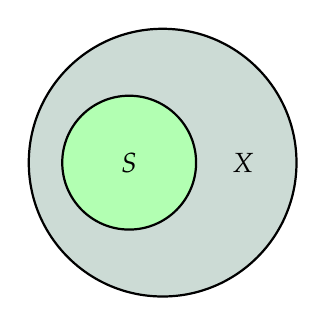
\begin{tikzpicture}[scale=0.85]
	\begin{scope}
	\filldraw[fill=forest,fill opacity=1/5,thick]   (0:0) circle (2);
    \filldraw[fill=green!30!white,thick] (0:-0.5) circle (1);
    \end{scope}
%\draw[thick] (-3,-2.5) rectangle (3,2.5);
\node at (0:1.2)    {$X$};
\node at (0:-0.5)    {$S$};
\end{tikzpicture}\]
Any set $X$ always has two subsets: itself and the empty set.
\end{definition}

\vspace*{1em}

\begin{example}
Let $B = \set{\emptyset,\set{\emptyset},1,2,\set{1,2}}$, then
\begin{align*}
\emptyset \in B,&\ \text{ so } \set{\emptyset} \subseteq B & \set{\emptyset} \in B,&\ \text{ so } \set{\set{\emptyset}} \subseteq B & 1,\,2 \in B,&\ \text{ so } \set{1,2} \subseteq B
\end{align*}
Also, $\set{1,2} \in B$ and $\emptyset,\,B \subseteq B$ as always.

\begin{dangerbend}
This example highlights a common error. We note that $\set{1,2} \subseteq B$ since $1$ and $2$ are \emph{elements} of $B$. But also $\set{1,2} \in B$, since $\set{1,2}$ is also an element of $B$.\\[0.5em]
Being an element means it itself is listed, as is, in a set; while being a subset means \emph{the elements of the subset} are listed as is. For example, take $C = \set{1,2,3}$; then $\set{1,2} \subseteq C$ but $\set{1,2} \notin C$ since the set $\set{1,2}$ is not an element of $C$.
\end{dangerbend}
\end{example}

\vspace*{1em}

We now use the notion of subsets to define what it means for two sets to be equal.
\begin{definition}[Equality of Sets]\label{equality-sets}
We say two sets $A$ and $B$ are equal if $A \subseteq B$ and $B \subseteq A$, and we denote it $A = B$.
\end{definition}

\vspace*{1em}

\begin{definition}[Proper Subsets]
A set $S$ is called a \cdef{proper\ subset} of $X$ if $S \subseteq X$ and $S \neq X$. We denote this as $S \subset X$ or $S \subsetneq X$. In other words, $S$ is a subset that is ``strictly smaller than $X$''.\\[0.5em]
If the set is non-empty, then it has a proper subset -- the empty set.
\end{definition}

\vspace*{1em}

\begin{definition}[Power Set]\label{power-set}
The \cdef{power\ set} of a set $X$ is the set of \emph{all} subsets of $X$, including $X$ and $\emptyset$. We denote it $\mathscr{P}(X)$.\\[0.5em]
For several reasons, the power set is also denoted as $2^X$, one reason is revealed below.
\end{definition}

%\vspace*{1em}

\begin{example}
Let's compute power sets of some sets.
\begin{itemize}[itemsep=0.5em]
\item[(1)] Let $A = \set{1,2,3}$, so $\abs{A} = 3$.
\begin{align*}
\emptyset \subseteq A&\\[0.5em]
1 \in A&, \text{ so } \set{1} \subseteq A\\[0.5em]
1,\,2 \in A&, \text{ so } \set{1,2} \subseteq A\\[0.5em]
1,\,2,\,3 \in A&, \text{ so } A = \set{1,2,3} \subseteq A
\end{align*}
We then get
\[\mathscr{P}(A) = \set{\emptyset,\set{1},\set{2},\set{3},\set{1,2},\set{2,3},\set{1,3},\set{1,2,3}}\]
Note that $\abs{\mathscr{P}(A)} = 8 = 2^3 = 2^{\abs{A}}$.

\item[(2)] Let $A = \set{1,\set{2}}$, so $\abs{A} = 2$. We have
\[\mathscr{P}(A) = \set{\emptyset,\set{1},\set{\set{2}},\set{1,\set{2}}}\]
$\abs{\mathscr{P}(A)} = 4 = 2^2 = 2^{\abs{A}}$.

\item[(3)] Let $A = \emptyset$, so $\abs{A} = 0$. We have
\[B = \mathscr{P}(A) = \set{\emptyset},\quad \abs{\mathscr{P}(A)} = 1 = 2^0 = 2^{\abs{A}}\]
What about $\mathscr{P}(B)$? We have
\[C = \mathscr{P}(B) = \set{\emptyset,\set{\emptyset}}\]
Finally,
\[\mathscr{P}(C) = \set{\emptyset,\set{\emptyset},\set{\set{\emptyset}},\set{\emptyset,\set{\emptyset}}}\]
\end{itemize}

\vspace*{1em}

\begin{remark}
It's true in general that $\abs{\mathscr{P}(X)} = 2^{\abs{X}}$, for any set $X$.
\end{remark}
\end{example}

\vspace*{2em}

\begin{mdframed}
\begin{center}
{\Large Set Operations}\label{set-operations}
\end{center}
\end{mdframed}

We assume all the sets in the section are subsets of some set $U$, labelled the ``universal set''.
\begin{definition}[Set Operations]
Let $A,\,B \subseteq U$.
\begin{itemize}[itemsep=1em]
\item The \cdef{union} of $A$ and $B$ is the set
\[A \cup B = \setp{x \in U}{x \in A \text{ \emph{or} } x \in B}\]
Here our use of ``or'' allows the possibility of $x$ being in both $A$ and $B$.

\item The \cdef{intersection} of $A$ and $B$ is the set
\[A \cap B = \setp{x \in U}{x \in A \text{ \emph{and} } x \in B}\]\newpage
It is clear definitionally that we always have $A \cap B \subseteq A \cup B$.
\[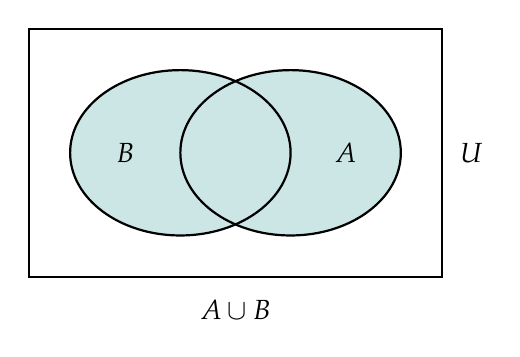
\begin{tikzpicture}[scale=0.7]
	\def\firstcircle{(0:1) ellipse (2cm and 1.5cm)};
    \def\secondcircle{(0:-1) ellipse (2cm and 1.5cm)};
	\begin{scope}
	\fill[white!80!teal] (0:1) ellipse (2cm and 1.5cm);
    \fill[white!80!teal] (0:-1) ellipse (2cm and 1.5cm);
    \end{scope}    
\draw[thick] \firstcircle;
\draw[thick] \secondcircle;
\node at (0:2)    {$A$};
\node at (0:-2)    {$B$};
\draw[thick] (-3.75,-2.25) rectangle (3.75,2.25);
\node[right,xshift=3pt] at (3.75,0){$U$};
\node[below,yshift=-5pt] at (0,-2.25){$A \cup B$};
\end{tikzpicture}\qquad
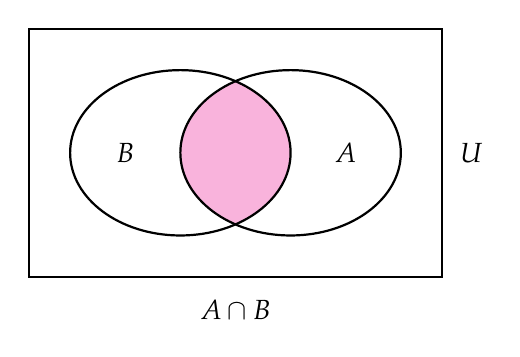
\begin{tikzpicture}[scale=0.7]
	\def\firstcircle{(0:1) ellipse (2cm and 1.5cm)};
    \def\secondcircle{(0:-1) ellipse (2cm and 1.5cm)};
	\begin{scope}
    \clip \firstcircle;
    \fill[white!70!magenta] \secondcircle;
    \end{scope}    
\draw[thick] \firstcircle;
\draw[thick] \secondcircle;
\node at (0:2)    {$A$};
\node at (0:-2)    {$B$};
\draw[thick] (-3.75,-2.25) rectangle (3.75,2.25);
\node[right,xshift=3pt] at (3.75,0){$U$};
\node[below,yshift=-5pt] at (0,-2.25){$A \cap B$};
\end{tikzpicture}\]

\item The \cdef{difference} of $A$ and $B$ is the set
\[A\setminus B = A - B = \setp{x \in U}{x \in A \text{ \emph{and} } x \notin B}\]
That is, it is the set that's left when we remove the part of $B$ that belonged to $A$. Similarly, we can also consider the set that's left when we remove the part of $A$ that belonged to $B$
\[B\setminus A = B - A = \setp{x \in U}{x \in B \text{ \emph{and} } x \notin A}\]
A related operation is the \cdef{symmetric\ difference} defined as
\[A\, \triangle\, B = (A \setminus B) \cup (B \setminus A)\]
\[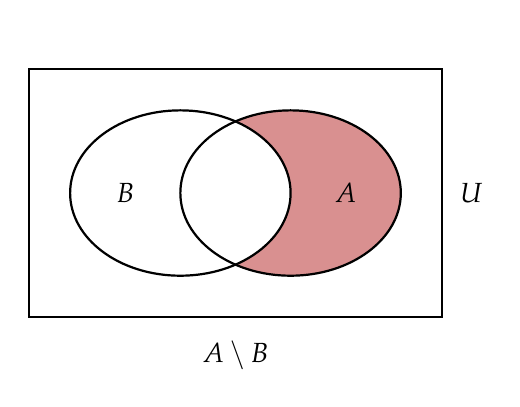
\begin{tikzpicture}[scale=0.7]
	\def\firstcircle{(0:1) ellipse (2cm and 1.5cm)};
    \def\secondcircle{(0:-1) ellipse (2cm and 1.5cm)};
    	\begin{scope}[even odd rule]
    		\clip \secondcircle (-2,-2) rectangle (3,3);
    		\fill[firebrick!50!white] \firstcircle;
	\end{scope}
\draw[thick] \firstcircle;
\draw[thick] \secondcircle;
\node at ( 0:2)    {$A$};
\node at (0:-2)    {$B$};
\draw[thick] (-3.75,-2.25) rectangle (3.75,2.25);
\node[right,xshift=3pt] at (3.75,0){$U$};
\node[below,yshift=-5pt] at (0,-2.25){$A \setminus B$};
\end{tikzpicture} \qquad
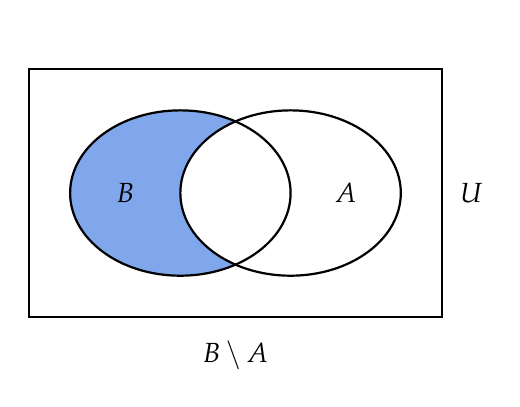
\begin{tikzpicture}[scale=0.7]
	\def\firstcircle{(0:1) ellipse (2cm and 1.5cm)};
    \def\secondcircle{(0:-1) ellipse (2cm and 1.5cm)};
    	\begin{scope}[even odd rule]
    		\clip \firstcircle (2,-2) rectangle (-3,3);
    		\fill[newblue!50!white] \secondcircle;
	\end{scope}
\draw[thick] \secondcircle;
\draw[thick] \firstcircle;
\node at ( 0:2)    {$A$};
\node at (0:-2)    {$B$};
\draw[thick] (-3.75,-2.25) rectangle (3.75,2.25);
\node[right,xshift=3pt] at (3.75,0){$U$};
\node[below,yshift=-5pt] at (0,-2.25){$B \setminus A$};
\end{tikzpicture}\]
\[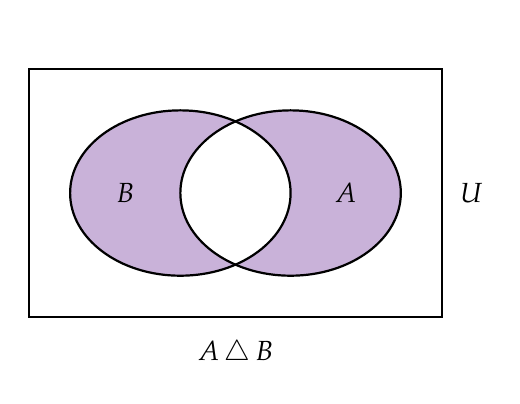
\begin{tikzpicture}[scale=0.7]
	\def\firstcircle{(0:1) ellipse (2cm and 1.5cm)};
    \def\secondcircle{(0:-1) ellipse (2cm and 1.5cm)};
	\begin{scope}[even odd rule]
    		\clip \secondcircle (-2,-2) rectangle (3,3);
    		\fill[white!70!indigo] \firstcircle;
	\end{scope}  
	\begin{scope}[even odd rule]
    		\clip \firstcircle (2,-2) rectangle (-3,3);
    		\fill[white!70!indigo] \secondcircle;
	\end{scope}
\draw[thick] \firstcircle;
\draw[thick] \secondcircle;
\node at ( 0:2)    {$A$};
\node at (0:-2)    {$B$};
\draw[thick] (-3.75,-2.25) rectangle (3.75,2.25);
\node[right,xshift=3pt] at (3.75,0){$U$};
\node[below,yshift=-5pt] at (0,-2.25){$A\, \triangle\, B$};
\end{tikzpicture}\]

\item The \cdef{complement} of $A$ in $U$ is the set \[A^c = \overline{A} = \setp{x \in U}{x \notin A}\]
That is, it is the set of exactly those elements in $U$ that don't belong to $A$.
\[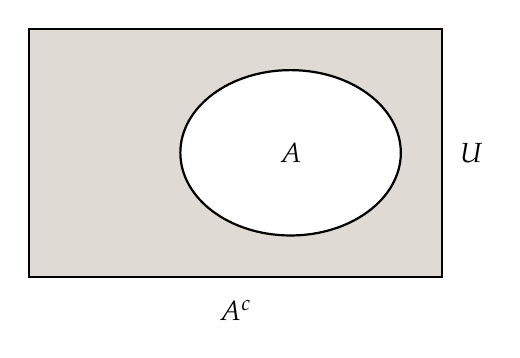
\begin{tikzpicture}[scale=0.7]
	\def\firstcircle{(0:1) ellipse (2cm and 1.5cm)};
\filldraw[fill=white!80!dirt,thick] (-3.75,-2.25) rectangle (3.75,2.25);
\filldraw[fill=white,thick] \firstcircle;
\node at (0:1)    {$A$};
\node[right,xshift=3pt] at (3.75,0){$U$};
\node[below,yshift=-5pt] at (0,-2.25){$A^c$};
\end{tikzpicture}\]
\end{itemize}
\end{definition}

\vspace*{1em}

\begin{proposition}\label{prop:set-id}
We have the following identities
\begin{itemize}
\item[(1)] $A \setminus B = A \cap B^c$
\item[(2)] $(A \cap B)^c = A^c \cup B^c$
\item[(3)] $(A \cup B)^c = A^c \cap B^c$
\end{itemize}
\end{proposition}
\begin{proof}
We give a ``proof by diagram'' for (1)

\begin{minipage}{0.5\textwidth}
\[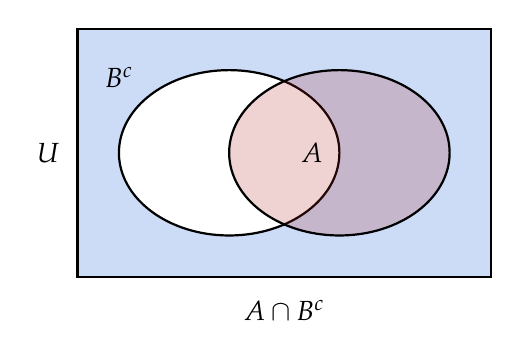
\begin{tikzpicture}[scale=0.7]
\filldraw[fill=newblue,fill opacity=1/5,thick] (-3.75,-2.25) rectangle (3.75,2.25);
	\def\firstcircle{(0:1) ellipse (2cm and 1.5cm)};
    \def\secondcircle{(0:-1) ellipse (2cm and 1.5cm)};
\filldraw[fill=white,thick] \secondcircle;
\filldraw[fill=firebrick,fill opacity=1/5,thick] \firstcircle;
\node at (0:0.5)    {$A$};
\node[above,yshift=2em] at (0:-3)    {$B^c$};
\node[left,xshift=-3pt] at (-3.75,0){$U$};
\node[below,yshift=-5pt] at (0,-2.25){$A \cap B^c$};
\end{tikzpicture}\]
\end{minipage}$=$
\begin{minipage}{0.5\textwidth}
\[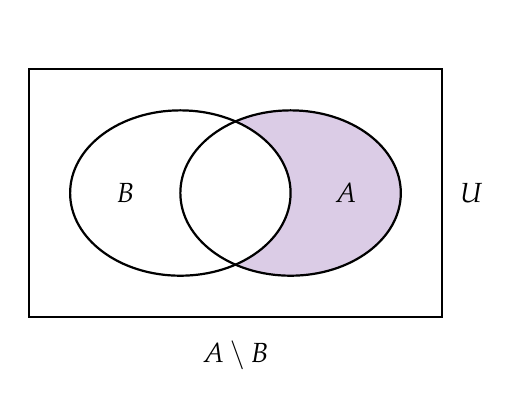
\begin{tikzpicture}[scale=0.7]
	\def\firstcircle{(0:1) ellipse (2cm and 1.5cm)};
    \def\secondcircle{(0:-1) ellipse (2cm and 1.5cm)};
    	\begin{scope}[even odd rule]
    		\clip \secondcircle (-2,-2) rectangle (3,3);
    		\fill[indigo,opacity=1/5] \firstcircle;
	\end{scope}
\draw[thick] \firstcircle;
\draw[thick] \secondcircle;
\node at ( 0:2)    {$A$};
\node at (0:-2)    {$B$};
\draw[thick] (-3.75,-2.25) rectangle (3.75,2.25);
\node[right,xshift=3pt] at (3.75,0){$U$};
\node[below,yshift=-5pt] at (0,-2.25){$A \setminus B$};
\end{tikzpicture}\]
\end{minipage}
Try proving (2) and (3) similarly. Such diagrams are called \emph{Venn diagrams}. We will revisit (2) and (3) when we discuss \emph{de Morgan Laws}.
\end{proof}

\vspace*{2em}

\begin{mdframed}
\begin{center}
{\Large Indexed Collection of Sets}\label{indexed-collection}
\end{center}
\end{mdframed}

\begin{discussion}
For a finite collection of sets
\[\set{A_1,A_2,\ldots,A_n} = \set{A_i}_{i=1}^n = \set{A_i}_{i \in I},\; I = \set{1,2,\ldots,n}\]
we have
\begin{align*}
A_1 \cap A_2 \cap \cdots \cap A_n &= \bigcap_{i=1}^nA_i = \bigcap_{i\in I} A_i\\[0.5em]
A_1 \cup A_2 \cup \cdots \cup A_n &= \bigcup_{i=1}^nA_i = \bigcup_{i\in I} A_i
\end{align*}
That motivates us to consider an arbitrary collection of sets, indexed by an index set $I$.
\begin{align*}
\set{X_\alpha,A_\beta,A_\gamma,\ldots} &= \set{X_\alpha}_{\alpha \in I},\; I = \set{\alpha,\beta,\gamma,\ldots}\\[0.5em]
X_\alpha \cap X_\beta \cap X_\gamma \cap \cdots &= \bigcap_{\alpha \in I} X_\alpha\\[0.5em]
X_\alpha \cup X_\beta \cup X_\gamma \cup \cdots &= \bigcup_{\alpha \in I} X_\alpha
\end{align*}
Our set $I$ has no restrictions; in particular, it is allowed to infinite.
\end{discussion}

\vspace*{1em}

\begin{example}
Let our index set be $I = [1,\infty)$. For each $r \in I$, we consider the set
%\[X_r = \left(-\frac{1}{r},\frac{1}{r}\right)\]
\[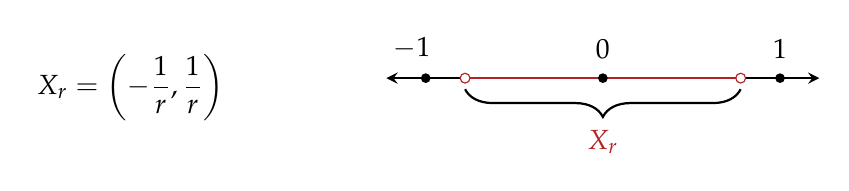
\begin{tikzpicture}
    \draw[<->,thick] (-2.75,0)--(2.75,0);
    \begin{scope}
        \draw[thick,firebrick] (-1.75,0)--(1.75,0);
%        \node[label=above:{$1/r$}](A) at (1.75,0) {};
%        \node[label=above:{$-1/r$}](B) at (-1.75,0) {};
		\fill[firebrick] (-1.75,0) circle (2pt);
		\fill[white] (-1.75,0) circle (1.5pt);
		\fill[firebrick] (1.75,0) circle (2pt);
		\fill[white] (1.75,0) circle (1.5pt);
		\fill[black] (2.25,0) circle (1.75pt);
		\fill[black] (-2.25,0) circle (1.75pt);
		\fill[black] (0,0) circle (1.75pt);
        \node[label=above:{$1$}](C) at (2.25,0) {};
        \node[label=above:{$-1$},xshift=-5pt](D) at (-2.25,0) {};
        \node[label=above:{$0$}](E) at (0,0) {};
        \draw [decorate,decoration={brace,amplitude=10pt,mirror,raise=4pt},yshift=0pt,thick]
(-1.75,0) -- (1.75,0) node [black,midway,below,yshift=-1.5em] {$\color{firebrick}X_r$};
        \node[label={$X_r = \left(-\dfrac{1}{r},\dfrac{1}{r}\right)$},yshift=-2.25em](F) at (-6,0) {};
    \end{scope}
\end{tikzpicture}\]
Then one can show that
\begin{align*}
\bigcap_{r \in I}X_r &= \set{0},\; \text{one point set}\\[0.5em]
\bigcup_{r \in I}X_r &= X_1 = (-1,1)
\end{align*}
\end{example}

\vspace*{2em}

\begin{mdframed}
\begin{center}
{\Large Partition of Sets}\label{partition}
\end{center}
\end{mdframed}

Let $A$ be a set, and $\mathscr{S} = \set{X_\alpha}_{\alpha \in I}$ a collection (or family) of non-empty subsets of $A$, where $I$ is some index set. That is, $\emptyset \neq X_\alpha \subseteq A$.

\begin{definition}[Partitions]
A collection $\mathscr{S}$ of subsets of $A$ is said to be a \cdef{partition} of $A$ if
\begin{itemize}
\item[(1)] $X_\alpha \cap X_\beta = \emptyset$ if $\alpha \neq \beta$ (we say $X_\alpha$ and $X_\beta$ are {\color{blue} (\cdef{mutually}) \cdef{disjoint}}); and
\item[(2)] $\bigcup_{\alpha \in I} X_\alpha = A$.
\end{itemize}
\begin{center}
\begin{minipage}{0.4\textwidth}
\[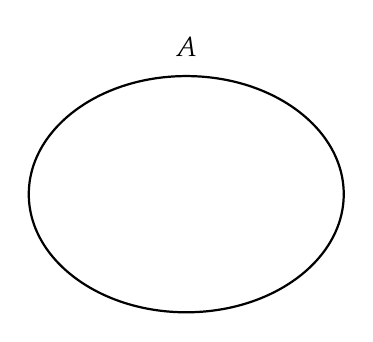
\begin{tikzpicture}
	\node[label=above:{$A$}](A) at (0,1.5) {};	
	\draw[thick] (0,0) ellipse (2cm and 1.5cm);
\end{tikzpicture}\]
\end{minipage}$\overset{\text{partition}}{\underset{\text{of $A$}}{\leadsto}}$
\begin{minipage}{0.4\textwidth}
\[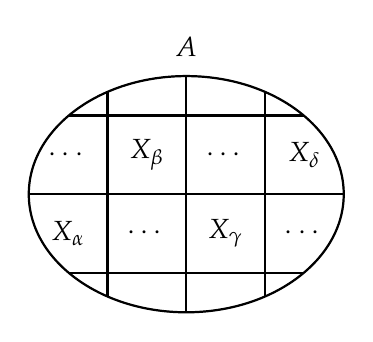
\begin{tikzpicture}
	\node[label=above:{$A$}](A) at (0,1.5) {};	
	\draw[thick] (0,0) ellipse (2cm and 1.5cm);
	\clip[draw] (0,0) ellipse (2cm and 1.5cm);
	\draw[thick] (-2,-2) grid (2,2);
	\node at (-1.5,-0.5) {$X_\alpha$};
	\node at (-0.5,+0.5) {$X_\beta$};
	\node at (+0.5,-0.5) {$X_\gamma$};
	\node at (+1.5,+0.5) {$X_\delta$};
	\node at (+0.5,+0.5) {$\cdots$};
	\node at (-0.5,-0.5) {$\cdots$};
	\node at (-1.5,+0.5) {$\cdots$};
	\node at (+1.5,-0.5) {$\cdots$};
\end{tikzpicture}\]
\end{minipage}
\end{center}

\vspace*{1em}

\begin{remark}
Later we will discuss the notion of ``equivalence relations'' and ``equivalence classes''. Partition of sets play an important role in this context.
\end{remark}
\end{definition}

%\vspace*{1em}

\begin{example}\label{example:modularith}\hfill
\begin{itemize}[itemsep=1em]
\item Let $A = \rr$ be the set of real numbers, we will produce a partition of $\rr$. For any integer $m$, consider the subset $X_m = [m,m+1)$ of $\rr$.
\[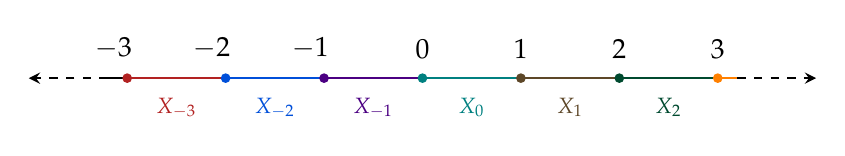
\begin{tikzpicture}
    \draw[thick] (-4,0)--(-3.75,0);
    \draw[->,thick,dashed] (-4,0)--(-5,0);
    \draw[->,thick,dashed] (4,0)--(5,0);
	\fill[firebrick] (-3.75,0) circle (1.75pt);
	\draw[thick,firebrick] (-3.75,0)--(-2.5,0);
	\fill[newblue] (-2.5,0) circle (1.75pt);
	\draw[thick,newblue] (-2.5,0)--(-1.25,0);
	\fill[indigo] (-1.25,0) circle (1.75pt);
	\draw[thick,indigo] (-1.25,0)--(0,0);
	\fill[teal] (0,0) circle (1.75pt);
	\draw[thick,teal] (0,0)--(1.25,0);
	\fill[dirt] (1.25,0) circle (1.75pt);
	\draw[thick,dirt] (1.25,0)--(2.5,0);
	\fill[forest] (2.5,0) circle (1.75pt);
	\draw[thick,forest] (2.5,0)--(3.75,0);
	\fill[orange] (3.75,0) circle (1.75pt);
	\draw[thick,orange] (3.75,0)--(4,0);

	\node[label=above:{$1$}] at (1.25,0) {};
	\node[label=above:{$2$}] at (2.5,0) {};
	\node[label=above:{$3$}] at (3.75,0) {};
	\node[label=above:{$-1$},xshift=-5pt] at (-1.25,0) {};
	\node[label=above:{$-2$},xshift=-5pt] at (-2.5,0) {};
	\node[label=above:{$-3$},xshift=-5pt] at (-3.75,0) {};
	\node[label=above:{$0$}] at (0,0) {};

	\node[label=below:{\color{firebrick}\footnotesize $X_{-3}$}] at (-3.125,0) {};
	\node[label=below:{\color{newblue}\footnotesize $X_{-2}$}] at (-1.875,0) {};
	\node[label=below:{\color{indigo}\footnotesize $X_{-1}$}] at (-0.625,0) {};
	\node[label=below:{\color{teal}\footnotesize $X_{0}$}] at (0.625,0) {};
	\node[label=below:{\color{dirt}\footnotesize $X_{1}$}] at (1.875,0) {};
	\node[label=below:{\color{forest}\footnotesize $X_{2}$}] at (3.125,0) {};
\end{tikzpicture}\]
Observe that
\[\begin{cases}
X_m \cap X_k = \emptyset, \text{ for any pair of integers $m \neq k$};\ \text{ and}\\[1em]
\rr = \bigcup_{m \in \zz}X_m\\[0.1em]
\end{cases}\]
Thus, $\setp{X_m}{m \in \zz}$ is a partition of $\rr$

\item Let $A = \zz$ be the set of integers, and let us also choose a positive integer $n$. We will produce a partition of $\zz$ with respect to $n$.\\[0.5em]
For an integer $r$ such that $0 \leq r < n$, consider the following subset of $\zz$
\begin{align*}
[r]_n &= \setp{k \in \zz}{\text{$k$ has remainder $r$ when divided by $n$}}\\[0.5em]
 &= \set{\ldots,-n + r,\,r,\,n + r,\,2n + r,\,3n + r,\ldots}\\[0.5em]
 &= \setp{k \in \zz}{k\equiv r \modar{n}}
\end{align*}
$[r]_n$ is an example of a \emph{congruence class modulo $n$}. Here for two integers $a,\,b \in \zz$ we say $a \equiv b \modar{n}$, ``$a$ is congruent to $b$ modulo $n$'', if $n$ divides $b - a$, written $n \mid (b-a)$.\\[0.5em]
For $n = 3,\ r = 0,1,2$
\begin{align*}
[0]_3 &= \set{\ldots,-6,-3,\,0,\,3,\,6,\,9,\ldots}\\[0.5em]
[1]_3 &= \set{\ldots,-5,-2,\,1,\,4,\,7,\,10,\ldots}\\[0.5em]
[2]_3 &= \set{\ldots,-4,-1,\,2,\,5,\,8,\,11,\ldots}
\end{align*}
Note that the remainder is always positive, for example $-4 = 3(-2) + 2$, which is why $-4 \in [2]_3$. Observe that
\[\begin{cases}
[0]_3 \cap [1]_3 = \emptyset,\;[0]_3 \cap [2]_3 = \emptyset,\;[1]_3 \cap [2]_3 = \emptyset;\ \text{ and}\\[1em]
[0]_3 \cup [1]_3 \cup [2]_3 = \zz\\[0.1em]
\end{cases}\]
Thus, $\set{[0]_3, [1]_3, [2]_3}$ is a partition of $\zz$.
\end{itemize}
We will revisit these example in greater detail later in the course.
\end{example}

\vspace*{2em}

\begin{mdframed}
\begin{center}
{\Large Cartesian Product}
\end{center}
\end{mdframed}

\begin{definition}[Cartesian Product]
For sets $A$ and $B$, we define the \cdef{cartesian\ product} $A \times B$ as the set of ordered pairs
\[A \times B = \setp{(a,b)}{a \in A,\ b \in B}\]
\end{definition}

%\vspace*{1em}

\begin{example}\hfill
\begin{itemize}[itemsep = 1em]
\item[(1)] Let $A = B = \rr$, the set of all real numbers.
\[\rr \times \rr = \setp{(x,y)}{x,\,y \in \rr}\]
Standard notation for this set is $\rr^2$, the Euclidean (or Cartesian) plane.

\item[(2)] $\rr \times \rr \times \rr = \setp{(x,y,z)}{x,\,y,\,z \in \rr}$. Standard notation for this set is $\rr^3$, the three-dimensional Euclidean space.

\item[(3)] Suppose $A = \set{1,2,3}$ and $B = \set{\text{red},\text{blue}}$, then
\[A \times B = \set{(1,\text{red}),(1,\text{blue}),(2,\text{red}),(2,\text{blue}),(3,\text{red}),(3,\text{blue})}\]
\end{itemize}
\end{example}

\vspace*{1em}

\begin{lemma}
$\abs{A \times B} = \abs{A}\cdot \abs{B}$ if both $A$ and $B$ are finite sets.
\end{lemma}
Things quickly get more subtle if $A$ and $B$ were infinite. 

\vspace*{1em}

\begin{remark}
If $A$ and $B$ are disjoint finite sets, that is, $A \cap B = \emptyset$, then
\[\abs{A \cup B} = \abs{A} + \abs{B}\]
But if $A$ or $B$ have infinitely many elements, strange phenomena can occur. For example, consider $A = \nn = \set{1,2,3,\ldots}$, the set of all positive integers, and $B = \set{0}$. Now $A$ is an infinite set, so let's say $\abs{A} = \infty$, and we of course have $\abs{B} = 1$.\\[0.5em]
Note that $A \cap B = \emptyset$, so we expect $\abs{A \cup B} = \abs{A} + \abs{B} = \infty + 1$. What is ``$\infty + 1$''? Does this make sense? We will develop the mathematical theory of infinity later in the course if we have time.
\end{remark}
\newpage

\section{Logic}
\vspace*{1em}

\begin{definition}[Statement]
A \cdef{statement} is a declarative sentence which can be objectively determined to be either \emph{true} or \emph{false}.
\end{definition}

%\vspace*{1em}

\begin{example}\hfill
\begin{itemize}
\item[(a)] \emph{The integer $11$ is divisible by $4$}. {\bf False} statement.
\item[(b)] \emph{The integer $11$ is a prime number}. {\bf True} statement.
\item[(c)] \emph{Is $10^{10}$ an integer?} This is a question, not a declarative sentence.
\item[(d)] \emph{The integer $10^{10}$ is big}. Not a statement, since the word ``big'' is subjective; the truth value $(\text{T},\text{F})$ may depend on individuals.
\end{itemize}
\end{example}

\vspace*{2em}

\begin{mdframed}
\begin{center}
{\Large Logical Connectives}
\end{center}
\end{mdframed}

\begin{definition}[Negation]
Given a statement $P$, the \cdef{negation} of $P$ is the statement \[\textbf{not $\mathbold{P}$},\quad \text{denoted $\neg P$}\]
It's characterised by the following \emph{truth table}
\begin{center}
{\renewcommand{\arraystretch}{1.5}%
\begin{tabular}{|>{\centering}m{1cm}|>{\centering\arraybackslash}m{1cm}|}
\hline
\rowcolor{lightgrey}
$P$ & $\neg P$\\
\hline
$\true$ & $\false$\\
\hline
$\false$ & $\true$\\
\hline
\end{tabular}
}
\end{center}
\end{definition}

\vspace*{1em}

\begin{example}
\begin{align*}
P:&\text{ The integer $11$ is odd.}\\[0.5em]
\neg P:&\text{ The integer $11$ is \emph{not} odd. $=$ The integer $11$ is even.}
\end{align*}
\end{example}

\vspace*{1em}

\begin{definition}[Disjunction]
Given statements $P$ and $Q$, the \cdef{disjunction} of $P$ and $Q$ is the statement \[\textbf{$\mathbold{P}$ or $\mathbold{Q}$},\quad \text{denoted $P \vee Q$}\] By definition, $P \vee Q$ is true if at least one of $P$ or $Q$ is true. Its truth table is
\begin{center}
{\renewcommand{\arraystretch}{1.5}%
\begin{tabular}{|>{\centering}m{1cm}|>{\centering}m{1cm}|>{\centering\arraybackslash}m{1cm}|}
\hline
\rowcolor{lightgrey}
$P$ & $Q$ & $P\vee Q$\\
\hline
$\true$ & $\true$ & $\true$\\
\hline
$\true$ & $\false$ & $\true$\\
\hline
$\false$ & $\true$ & $\true$\\
\hline
$\false$ & $\false$ & $\false$\\
\hline
\end{tabular}
}
\end{center}
\end{definition}

%\vspace*{1em}

\begin{example}
\begin{align*}
P:\text{$5$ is odd.} &\quad\true\\[0.5em]
Q:\text{$10$ is prime.} &\quad\false\\[0.5em]
P\vee Q:\text{$5$ is odd or $10$ is prime.} &\quad\true
\end{align*}
\end{example}

\vspace*{1em}

\begin{example}\label{example:pornot}
Let $P$ be any statement, then $\mathbold{P}$ or \textbf{not $\mathbold{P}$} is always true. We see this by looking at the truth table.
\begin{center}
{\renewcommand{\arraystretch}{1.5}%
\begin{tabular}{|>{\centering}m{1cm}|>{\centering}m{1cm}|>{\centering\arraybackslash}m{2cm}|}
\hline
\rowcolor{lightgrey}
$P$ & $\neg P$ & $P\vee (\neg P)$\\
\hline
$\true$ & $\false$ & $\true$\\
\hline
$\false$ & $\true$ & $\true$\\
\hline
\end{tabular}
}
\end{center}
We call statements that are always true a \emph{tautology}.
\end{example}

\vspace*{1em}

\begin{definition}[Conjunction]
Given statements $P$ and $Q$, the \cdef{conjunction} of $P$ and $Q$ is the statement \[\textbf{$\mathbold{P}$ and $\mathbold{Q}$},\quad \text{denoted $P \wedge Q$}\] By definition, $P \wedge Q$ is true only when both $P$ and $Q$ are true. Its truth table is
\begin{center}
{\renewcommand{\arraystretch}{1.5}%
\begin{tabular}{|>{\centering}m{1cm}|>{\centering}m{1cm}|>{\centering\arraybackslash}m{1cm}|}
\hline
\rowcolor{lightgrey}
$P$ & $Q$ & $P\vee Q$\\
\hline
$\true$ & $\true$ & $\true$\\
\hline
$\true$ & $\false$ & $\false$\\
\hline
$\false$ & $\true$ & $\false$\\
\hline
$\false$ & $\false$ & $\false$\\
\hline
\end{tabular}
}
\end{center}
\end{definition}

\vspace*{1em}

\begin{definition}[Implication]
Given statements $P$ and $Q$, the \cdef{implication} is the statement \[\textbf{if $\mathbold{P}$ then $\mathbold{Q}$},\quad \text{denoted $P \implies Q$}\]
In this statement, $P$ is called the \emph{hypothesis}, while $Q$ is called the \emph{conclusion}. Its truth table is
\begin{center}
{\renewcommand{\arraystretch}{1.5}%
\begin{tabular}{|>{\centering}m{1cm}|>{\centering}m{1cm}|>{\centering\arraybackslash}m{1.5cm}|}
\hline
\rowcolor{lightgrey}
$P$ & $Q$ & $P \implies Q$\\
\hline
$\true$ & $\true$ & $\true$\\
\hline
$\true$ & $\false$ & $\false$\\
\hline
$\false$ & $\true$ & $\true$\\
\hline
$\false$ & $\false$ & $\true$\\
\hline
\end{tabular}
}
\end{center}
When hypothesis $P$ is not satisfied $(\false)$, then whatever the conclusion $Q$ may be $(\true,\false)$, the implication $P \implies Q$ is true.
\end{definition}

%\vspace*{1em}

\begin{example}
\begin{align*}
P:&\text{ It is raining.}\\[0.5em]
Q:&\text{ I will stay at home.}\\[0.5em]
P\Rightarrow Q:&\text{ If it is raining, then I will stay at home.}
\end{align*}
\end{example}

\vspace*{1em}

\begin{definition}[Different Terminology for Implication]
The statement $P \Rightarrow Q$ is read in several different ways.
\begin{equation*}
  \left.\begin{aligned}
  \text{\emph{if $P$, then $Q$}}\\[0.5em]
  \text{\emph{$P$ implies $Q$}}\\[0.5em]
  \text{\emph{$Q$ if $P$}}\\[0.5em]
  \text{\emph{$P$ only if $Q$}}\\[0.5em]
  \text{$P$ is \emph{sufficient} for $Q$}\\[0.5em]
  \text{$Q$ is \emph{necessary} for $P$}\\
\end{aligned}\right\}\text{all mean $P \implies Q$}
\end{equation*}
\end{definition}

\vspace*{1.5em}

We have just seen four ways to create new statements from one or two given statements. In mathematics, however, we are often interested in declarative sentences containing variables and whose truth or falseness is only known once we have assigned values to the variables.
\begin{definition}[Open Sentences]
An \cdef{open\ sentence} is a declarative sentence which contains variables, where each variable can assume any value in a given set, called the \cdef{domain} of variables, which becomes a statement if variables are replaced by specific values. 
\end{definition}

\vspace*{1em}

\begin{example}
For $x \in \rr$, consider the statement $P(x):\abs{x} = 3$,
\begin{center}
{\renewcommand{\arraystretch}{1.5}%
\begin{tabular}{|>{\centering}m{1.5cm}|>{\centering}m{3cm}|>{\centering\arraybackslash}m{1cm}|}
\hline
$x = 1$ & $P(1) : \abs{1} = 3$ & $\false$\\
\hline
$x = -3$ & $P(-3) : \abs{-3} = 3$ & $\true$\\
\hline
$x = 2$ & $P(2) : \abs{2} = 3$ & $\false$\\
\hline
\end{tabular}
}
\end{center}
\end{example}

\vspace*{1em}

We can combine open sentences using $\neg,\,\vee,\,\wedge,\,\implies$ to make new open sentences.
\begin{example}
\begin{align*}
P(x):& \abs{x} = 3,\ x \in \rr & Q(x):& \abs{x} = -3,\ x \in \rr
\end{align*}
Consider then,
\begin{align*}
\neg P(x):& \abs{x} \neq 3 & \neg P(1) :& \abs{1} \neq 3 \quad (\true) \\[0.5em]
P(x) \vee Q(x):& \abs{x} = 3 \text{ or } x = -3 & P(3) \vee Q(3) :& \abs{3} = 3 \text{ or } 3 = -3 \quad (\false)\\
\end{align*}
Now consider,
\[Q(x) \implies P(x): \text{if $x = -3$, then $\abs{x} = 3$};\]
this is an open sentence. 
\begin{itemize}[leftmargin=4.5em,itemsep=1em]
\item[$x = -3$,] $Q(-3) \implies P(-3): \text{if $-3 = -3$, then $\abs{-3} = 3$}$.\\[0.5em]
Since both hypothesis and conclusion are true, this statement is $\true$. This is the \emph{everyday thought}.
\item[$x = 2$,] $Q(2) \implies P(2): \text{if $2 = -3$, then $\abs{2} = 3$}$.\\[0.5em]
Since the hypothesis is false, this implication statement is $\true$.
\item[$x \neq -3$,] since the hypothesis is false, the implication statement $Q(x) \implies P(x)$ is $\true$.
\end{itemize}
Thus, \emph{for all choices of $x \in \rr$}, the open sentence
\[Q(x) \implies P(x)\]
is true. In other words, the open sentence
\[\text{if $x = -3$, then $\abs{x} = 3$}\]
is true for $x = -3$ case, as well as for all other choices of values of $x$. In everyday logic, we only consider the case $x = -3$. The above open sentence is a true statement whether the value of $x$ is $-3$ or not.
\end{example}

\vspace*{1em}

\begin{definition}[Converse]
The implication $Q \implies P$ is called the \cdef{converse} of $P \implies Q$.
\end{definition}

\vspace*{1em}

\begin{definition}[Biconditional]
Given statements $P$ and $Q$, the \cdef{biconditional} of $P$ and $Q$ is the statement \[(P \implies Q) \wedge (Q \implies P),\quad \text{denoted $P \iff Q$}\]
That is, $P$ only if $Q$, and, $P$ if $Q$.\\
\\
We say,
\begin{equation*}
  \left\{\begin{aligned}
  &\text{$P$ if and only if $Q$ (abbreviated as $P$ iff $Q$)}\\[0.5em]
  &\text{$P$ is equivalent to $Q$}\\[0.5em]
  &\text{$P$ is necessary $(Q \implies P)$ and sufficient $(P \implies Q)$ for $Q$}\\ 
\end{aligned}\right.
\end{equation*}
The truth table is
\begin{center}
{\renewcommand{\arraystretch}{1.5}%
\begin{tabular}{|>{\centering}m{1cm}|>{\centering}m{1cm}|>{\centering}m{1.5cm}|>{\centering}m{1.5cm}|>{\centering\arraybackslash}m{3.75cm}|}
\hline
\rowcolor{lightgrey}
$P$ & $Q$ & $P \implies Q$ & $Q \implies P$ & $(P \implies Q) \wedge (Q \implies P)$\\
\hline
$\true$ & $\true$ & $\true$ & $\true$ & $\true$\\
\hline
$\true$ & $\false$ & $\false$ & $\true$ & $\false$\\
\hline
$\false$ & $\true$ & $\true$ & $\false$ & $\false$\\
\hline
$\false$ & $\false$ & $\true$ & $\true$ & $\true$\\
\hline
\end{tabular}
}
\end{center}
\vspace*{1em}
Note that $P \iff Q$ is true only when both $P$ and $Q$ are true or false.
\end{definition}

%\vspace*{1em}

\begin{remark}
Biconditional statements arise in mathematical definitions; the way to formally talk about that is to introduce the notion of \emph{characterization}. Suppose some concept or object is expressed via an open sentence $P(x)$ over a domain $S$, and suppose $Q(x)$ is another open sentence concerning the same concept over the same domain $S$. Then $P(x)$ is said to be characterized by $Q(x)$ if for every $x\in S$, the statement $P(x) \iff Q(x)$ is true. For example a characterization for odd numbers is \emph{a number $n$ is odd if and only if $n-1$ is even.}
\end{remark}

\vspace*{2em}

\begin{mdframed}
\begin{center}
{\Large Compound Statements}
\end{center}
\end{mdframed}

\begin{definition}[Compound Statements]
A \cdef{compound\ statement} is a statement consisting of at least one statement involving at least one logical connectives $(\neg,\,\wedge,\,\vee,\,\implies,\,\iff)$. Each statement in a compound statement is called a \cdef{component\ statement}. The biconditional $P \iff Q$ is an example with component statements $P \implies Q$ and $Q \implies P$
\end{definition}

\vspace*{1em}

\begin{definition}[Tautology and Contradiction]
A compound statement is called a \cdef{tautology} if it is \emph{true} for all possible combinations of truth values for its component statements. We will denote any tautology as $\top$.\\[0.5em]
A compound statement is called a \cdef{contradiction} if it is \emph{false} for all possible combinations of truth values for its component statements. We will denote any tautology as $\bot$.
\end{definition}

\vspace*{1em}

\begin{example}\label{example:tautcontr}\hfill
\begin{itemize}[itemsep=1em]
\item[(1)] We have seen in Example \ref{example:pornot} that $P \vee (\neg P)$ is a tautology.

\item[(2)] $P \wedge (\neg P)$ is a contradiction.
\begin{center}
{\renewcommand{\arraystretch}{1.5}%
\begin{tabular}{|>{\centering}m{1cm}|>{\centering}m{1cm}|>{\centering\arraybackslash}m{2cm}|}
\hline
\rowcolor{lightgrey}
$P$ & $\neg P$ & $P\wedge (\neg P)$\\
\hline
$\true$ & $\false$ & $\false$\\
\hline
$\false$ & $\true$ & $\false$\\
\hline
\end{tabular}
}
\end{center}

\item[(3)] $(P \wedge (P \implies Q)) \implies Q$, ``assume $P$ and also assume $P$ implies $Q$, then $Q$'' , is a tautology. We check by building the truth table.
\begin{center}
{\renewcommand{\arraystretch}{1.5}%
\begin{tabular}{|>{\centering}m{1cm}|>{\centering}m{1cm}|>{\centering}m{1.5cm}|>{\centering}m{2.5cm}|>{\centering\arraybackslash}m{3.75cm}|}
\hline
\rowcolor{lightgrey}
$P$ & $Q$ & $P \implies Q$ & $P \wedge (P \implies Q)$ & $(P \wedge (P \implies Q)) \implies Q$\\
\hline
$\true$ & $\true$ & $\true$ & $\true$ & $\true$\\
\hline
$\true$ & $\false$ & $\false$ & $\false$ & $\true$\\
\hline
$\false$ & $\true$ & $\true$ & $\false$ & $\true$\\
\hline
$\false$ & $\false$ & $\true$ & $\false$ & $\true$\\
\hline
\end{tabular}
}
\end{center}

\item[(3)] $S:((P \implies Q) \wedge (Q \implies R)) \implies (P \implies R)$ is a tautology.
%\begin{tabular}{|>{\centering\arraybackslash}m{6cm}|}
%\hline
%\rowcolor{lightgrey}
%$((P \implies Q) \wedge (Q \implies R)) \implies (P \implies R)$\\
%\hline
%$\true$\\
%\hline
%$\true$\\
%\hline
%$\true$\\
%\hline
%$\true$\\
%\hline
%$\true$\\
%\hline
%$\true$\\
%\hline
%$\true$\\
%\hline
%$\true$\\
%\hline
%\end{tabular}
\end{itemize} 
\begin{center}
{\renewcommand{\arraystretch}{1.5}%
\begin{tabular}{|>{\centering}m{0.5cm}|>{\centering}m{0.5cm}|>{\centering}m{0.5cm}|>{\centering}m{1cm}|>{\centering}m{1cm}|>{\centering}m{3cm}|>{\centering}m{1cm}|>{\centering\arraybackslash}m{5cm}|}
\hline
\rowcolor{lightgrey}
{\footnotesize $P$} & {\footnotesize $Q$} & {\footnotesize $R$} & {\footnotesize $P \implies Q$} & {\footnotesize $Q \implies R$} & {\footnotesize $(P \implies Q) \wedge (Q \implies R)$} & {\footnotesize $P \implies R$} & {\footnotesize $((P \implies Q) \wedge (Q \implies R)) \implies (P \implies R)$}\\
\hline
$\true$ & $\true$ & $\true$ & $\true$ & $\true$ & $\true$ & $\true$ & $\true$\\
\hline
$\true$ & $\true$ & $\false$ & $\true$ & $\false$ & $\false$ & $\false$ & $\true$\\
\hline
$\true$ & $\false$ & $\true$ & $\false$ & $\true$ & $\false$ & $\true$ & $\true$\\
\hline
$\true$ & $\false$ & $\false$ & $\false$ & $\true$ & $\false$ & $\false$ & $\true$\\
\hline
$\false$ & $\true$ & $\true$ & $\true$ & $\true$ & $\true$ & $\true$ & $\true$\\
\hline
$\false$ & $\true$ & $\false$ & $\true$ & $\false$ & $\false$ & $\true$ & $\true$\\
\hline
$\false$ & $\false$ & $\true$ & $\true$ & $\true$ & $\true$ & $\true$ & $\true$\\
\hline
$\false$ & $\false$ & $\false$ & $\true$ & $\true$ & $\true$ & $\true$ & $\true$\\
\hline
\end{tabular}
}
\end{center}
\end{example}

\vspace*{2em}

\begin{mdframed}
\begin{center}
{\Large Logical Equivalence}
\end{center}
\end{mdframed}

\begin{definition}[Logical Equivalence]
Two compound statements $R$ and $S$ are \cdef{logically\ equivalent} if they have the same truth value for all possible combinations of truth values for its component statements. We denote this as
\[R \equiv S\]
$R$ and $S$ are logically equivalent if and only if the biconditional statement $R \iff S$ is a tautology.  
\end{definition}

\vspace*{1em}

\begin{theorem}\label{theorem:impliesequiv}
Let $P$ and $Q$ be statements, then
\[(P \implies Q) \equiv ((\neg P) \vee Q)\]
\end{theorem}
\begin{proof}
We build the truth table and compare the truth values.
\begin{center}
{\renewcommand{\arraystretch}{1.5}%
\begin{tabular}{|>{\centering}m{1cm}|>{\centering}m{1cm}|>{\centering}m{1cm}||>{\centering}m{1.5cm}||>{\centering}m{2cm}||>{\centering\arraybackslash}m{4.25cm}|}
\hline
\rowcolor{lightgrey}
$P$ & $Q$ & $\neg P$ & $P \implies Q$ & $(\neg P) \vee Q$ & $(P \implies Q) \iff ((\neg P) \vee Q)$\\
\hline
$\true$ & $\true$ & $\false$ & $\true$ & $\true$ & $\true$\\
\hline
$\true$ & $\false$ & $\false$ & $\false$ & $\false$ & $\true$\\
\hline
$\false$ & $\true$ & $\true$ & $\true$ & $\true$ & $\true$\\
\hline
$\false$ & $\false$ & $\true$ & $\true$ & $\true$ & $\true$\\
\hline
\end{tabular}
}
\end{center}
So comparing the truth values of $P \implies Q$ and $(\neg P) \vee Q$ we see $(P \implies Q) \equiv ((\neg P) \vee Q)$, and the final column also tells us that $(P \implies Q) \iff ((\neg P) \vee Q)$ is a tautology.
\end{proof}

\vspace*{1em}

\begin{theorem}[Laws of Logical Equivalence]
Let $P,\,Q$ and $R$ be statements, and let $\top$ and $\bot$ be a tautology and contradiction respectively, then
\begin{itemize}[itemsep=1.5em]
\item[(L1)] Identity laws
\begin{align*}
P \vee \bot &\equiv P\\[0.5em]
P \wedge \top &\equiv P
\end{align*}

\item[(L2)] Domination laws
\begin{align*}
P \vee \top &\equiv \top\\[0.5em]
P \wedge \bot &\equiv \bot
\end{align*}

\item[(L3)] Double Negation law
\begin{align*}
\neg(\neg P) &\equiv P
\end{align*}


\item[(L4)] Commutative laws
\begin{align*}
P \vee Q &\equiv Q \vee P\\[0.5em]
P \wedge Q &\equiv Q \wedge P
\end{align*}

\item[(L5)] Associative laws
\begin{align*}
P \vee (Q \vee R) &\equiv (P \vee Q) \vee R\\[0.5em]
P \wedge (Q \wedge R) &\equiv (P \wedge Q) \wedge R
\end{align*}

\item[(L6)] Distributive laws
\begin{align*}
P\, {\color{newblue}\vee}\, (Q\, {\color{firebrick}\wedge}\, R) &\equiv (P\, {\color{newblue}\vee}\, Q)\, {\color{firebrick}\wedge}\, (P\, {\color{newblue}\vee}\, R)\\[0.5em]
P\, {\color{firebrick}\wedge}\, (Q\, {\color{newblue}\vee}\, R) &\equiv (P\, {\color{firebrick}\wedge}\, Q)\, {\color{newblue}\vee}\, (P\, {\color{firebrick}\wedge}\, R)
\end{align*}

\item[(L7)] De Morgan's laws
\begin{align*}
\text{(L7a)}\quad\neg (P \vee Q) &\equiv (\neg P) \wedge (\neg Q)\\[0.5em]
\text{(L7b)}\quad\neg (P \wedge Q) &\equiv (\neg P) \vee (\neg Q)
\end{align*}
\end{itemize}
\end{theorem}
\vspace*{0.5em}
\begin{proof}
We simply have to build the appropriate truth tables. For example, for (L7a) we have\\
\begin{center}
{\renewcommand{\arraystretch}{1.5}%
\begin{tabular}{|>{\centering}m{1cm}|>{\centering}m{1cm}|>{\centering}m{1.5cm}||>{\centering}m{1.75cm}||>{\centering}m{1cm}|>{\centering}m{1cm}||>{\centering\arraybackslash}m{2.5cm}|}
\hline
\rowcolor{lightgrey}
$P$ & $Q$ & $P \vee Q$ & $\neg(P \vee Q)$ & $\neg P$ & $\neg Q$ & $(\neg P) \wedge (\neg Q)$\\
\hline
$\true$ & $\true$ & $\true$ & $\false$ & $\false$ & $\false$ & $\false$\\
\hline
$\true$ & $\false$ & $\true$ & $\false$ & $\false$ & $\true$ & $\false$\\
\hline
$\false$ & $\true$ & $\true$ & $\false$ & $\true$ & $\false$ & $\false$\\
\hline
$\false$ & $\false$ & $\false$ & $\true$ & $\true$ & $\true$ & $\true$\\
\hline
\end{tabular}
}
\end{center}
\vspace*{0.5em}
Comparing the truth values, we see $\neg (P \vee Q) \equiv (\neg P) \wedge (\neg Q)$.
\end{proof}

\vspace*{1em}

\begin{example}
Show $\neg(P \implies Q) \equiv (P \wedge (\neg Q))$
\begin{itemize}
\item[] \emph{Method 1.} Build truth table
\begin{center}
{\renewcommand{\arraystretch}{1.5}%
\begin{tabular}{|>{\centering}m{1cm}|>{\centering}m{1cm}|>{\centering}m{1.5cm}|>{\centering}m{2cm}|>{\centering}m{1cm}|>{\centering\arraybackslash}m{2cm}|}
\hline
\rowcolor{lightgrey}
$P$ & $Q$ & $P \implies Q$ & $\neg(P \implies Q)$ & $\neg Q$ & $P \wedge \neg Q$\\
\hline
$\true$ & $\true$ & $\true$ & $\false$ & $\false$ & $\false$\\
\hline
$\true$ & $\false$ & $\false$ & $\true$ & $\true$ & $\true$\\
\hline
$\false$ & $\true$ & $\true$ & $\false$ & $\false$ & $\false$\\
\hline
$\false$ & $\false$ & $\true$ & $\false$ & $\true$ & $\false$\\
\hline
\end{tabular}
}
\end{center}
Comparing the truth values, we see $\neg(P \implies Q) \equiv (P \wedge (\neg Q))$.
\item[] \emph{Method 2.} Use the logical equivalence laws
\begin{align*}
\neg(P \implies Q) &\equiv \neg ((\neg P) \vee Q) && \text{by Theorem \ref{theorem:impliesequiv}}\\[0.5em]
 &\equiv \neg(\neg P) \wedge (\neg Q) && \text{by De Morgan's laws}\\[0.5em]
 &\equiv P \wedge (\neg Q) && \text{by Double Negation law}
\end{align*}
\end{itemize}
\end{example}

\vspace*{1em}

\begin{example}
Show $((\neg Q) \implies (P \wedge \neg P)) \equiv Q$
\begin{itemize}
\item[] \emph{Method 1.} Build truth table (sure, but a tedious way)
\item[] \emph{Method 2.} Use the logical equivalence laws
\begin{align*}
((\neg Q) \implies (P \wedge \neg P)) &\equiv (\neg(\neg Q) \vee (P \wedge \neg P)) && \text{by Theorem \ref{theorem:impliesequiv}}\\[0.5em]
 &\equiv (\neg(\neg Q) \vee \bot) && \text{by Example \ref{example:tautcontr} (2)}\\[0.5em]
 &\equiv \neg(\neg Q) && \text{by Identity laws}\\[0.5em]
 &\equiv Q && \text{by Double Negation law}
\end{align*}
\end{itemize}
The above statement says ``if negation of $Q$ implies a contradiction, then $Q$ is true''.
\end{example}

\vspace*{1em}

\begin{example}
Show $((P \wedge \neg Q) \implies (R \wedge \neg R)) \equiv (P \implies Q)$
\begin{itemize}
\item[] \emph{Method 1.} Build truth table (sure, but a tedious way)
\item[] \emph{Method 2.} Use the logical equivalence laws
\begin{align*}
((P \wedge \neg Q) \implies (R \wedge \neg R)) &\equiv (\neg(P \wedge \neg Q) \vee (R \wedge \neg R)) && \text{by Theorem \ref{theorem:impliesequiv}}\\[0.5em]
 &\equiv (\neg(P \wedge \neg Q) \vee \bot) && \text{by Example \ref{example:tautcontr} (2)}\\[0.5em]
 &\equiv \neg(P \wedge \neg Q) && \text{by Identity laws}\\[0.5em]
 &\equiv \neg P \vee \neg(\neg Q) && \text{by De Morgan's laws}\\[0.5em]
 &\equiv \neg P \vee Q && \text{by Double Negation law}\\[0.5em]
 &\equiv P \implies Q && \text{by Theorem \ref{theorem:impliesequiv}}
\end{align*}
\end{itemize}
The above equivalence is the ``\emph{proof by contradiction}''. To show $P \implies Q$, do the following. Assume the hypothesis $P$ is true but the conclusion $Q$ is false. If you can deduce a contradiction $(R \wedge \neg R)$, then $P \implies Q$ is true.
\end{example}

\vspace*{2em}

\begin{mdframed}
\begin{center}
{\Large Quantified Statements}
\end{center}
\end{mdframed}

\begin{discussion}[Quantifiers]
Let $P(x)$ be an open sentence over a domain $S$. Recall that $P(x)$ becomes a statement once we specify an $x \in S$. We can produce specific kinds of statements from this open sentence called \cdef{quantified\ statements}.
\begin{itemize}[itemsep=1em]
\item \emph{for all $x \in S,\ P(x)$ is true}.\\[0.5em]
The phrase ``for all'' is referred to as the \cdef{universal\ quantifier} and is denoted by the symbol $\forall$. Other ways to express the universal quantifier are ``for every'', ``for any'' and ``for each''. Symbolically, we express the universally quantified statement as
\[\forall x \in S,\ P(x)\]
The statement is true if $P(x)$ is true for every $x \in S$.

\item \emph{there exists $x \in S$ such that $P(x)$ is true}.\\[0.5em]
The phrase ``there exists'' is referred to as the \cdef{existential\ quantifier} and is denoted by the symbol $\exists$. Symbolically, we express the existentially quantified statement as
\[\exists x \in S,\ P(x)\]
The statement is true if $P(x)$ is true for at least one $x \in S$.
\end{itemize}
\end{discussion}

\vspace*{1em}

\begin{example}
Consider the open sentence
\[P(n):n^2 + n \text{ is even}\]
with domain $\zz$, the set of integers. Then, we have statements
\begin{align*}
\text{for all $n \in \zz$, $n^2 + n$ is even.}&\qquad \forall n \in \zz,\ P(n) \qquad (\true)\\[0.5em]
\text{there exists an $n \in \zz$ such that $n^2 + n$ is even.}&\qquad \exists n \in \zz,\ P(n) \qquad (\true)
\end{align*}
\end{example}

\vspace*{1em}

\begin{discussion}[Negation of Quantified Statements]\hfill
\begin{align*}
\neg (\forall x\in S,\ P(x)) &= \text{it is not the case that for all $x \in S$, $P(x)$ is true.}\\[0.5em]
 &= \text{there exists $x \in S$ such that $P(x)$ is false.}\\[0.5em]
 &= \exists x\in S,\ \neg P(x)\\[1em]
 \neg (\exists x\in S,\ P(x)) &= \text{it is not the case that there exists $x \in S$ such that $P(x)$ is true.}\\[0.5em]
 &= \text{for all $x \in S$, $P(x)$ is false.}\\[0.5em]
 &= \forall x\in S,\ \neg P(x)
\end{align*}
\end{discussion}

%\vspace*{1em}

\begin{discussion}[Summarising Negation Rules]
\begin{equation*}
\text{under negation}\left\{\begin{aligned}
	\wedge &\leftrightarrow \vee\\[0.5em]
	\forall &\leftrightarrow \exists\\[0.5em]
	P(x) &\leftrightarrow \neg P(x)
\end{aligned}\right.
\end{equation*}
\end{discussion}

\vspace*{1em}

\begin{discussion}[Double Quantifiers and their Negation]
Let $x \in S$ and $y \in T$ be variables. Consider,
\begin{align*}
\forall x \in S,\ \forall y \in T,\ P(x,y)\\[0.5em]
\text{\emph{for all $x \in S$ and $y \in T$, $P(x,y)$ is true.}}
\end{align*}
The negation is
\begin{align*}
\neg(\forall x \in S,\ \forall y \in T,\ P(x,y)) &\equiv \exists x \in S,\neg(\forall y \in T,\ P(x,y))\\[0.5em]
&\equiv \exists x \in S,\ \exists y \in T,\ \neg P(x,y)\\
\end{align*}
For example, consider the statement \emph{for all $x \in \rr$ and $y \in \rr$, $x^2 + y^2 > 0$.}
\[\text{Negation: \emph{there exists $x \in \rr$ and $y \in \rr$ such that $x^2 + y^2 \leq 0$}.}\]
This is $\true$, since for $x = y = 0$ we have $x^2 + y^2 = 0$.\\
\\
Similarly,
\begin{align*}
\neg(\forall x \in S,\ \exists y \in T,\ P(x,y)) &\equiv \exists x \in S,\neg(\exists y \in T,\ P(x,y))\\[0.5em]
&\equiv \exists x \in S,\ \forall y \in T,\ \neg P(x,y)
\end{align*}
In other words,
\begin{align*}
\neg(\text{for all $x \in S$,} &\text{ there exists $y \in T$ such that $P(x,y)$ is true})\\[0.5em]
&\equiv \text{there exists $x \in S$ such that for all $y \in T$, $P(x,y)$ is true}\\
\end{align*}
Finally,
\begin{align*}
\neg(\exists x \in S,\ \forall y \in T,\ P(x,y)) &\equiv \forall x \in S,\ \exists y \in T,\ \neg P(x,y)\\[0.5em]
\neg(\exists x \in S,\ \exists y \in T,\ P(x,y)) &\equiv \forall x \in S,\ \forall y \in T,\ \neg P(x,y)
\end{align*}
\end{discussion}

\vspace*{1em}

\begin{example}[Finding Negation]
We'll negate the following statement
\[\emph{for all integers $a,b$, if their product is even, then $a$ is even or $b$ is even}\]
To find the negation, we identify the component statements and re-write symbolically. Consider the following open sentences over $\zz$ as the domain
\begin{align*}
P(x,y)&:\text{the product $xy$ is even.}\\[0.5em]
Q(x)&:\text{$x$ is even.}
\end{align*}
Using these open sentences, our statement is
\[\forall a\in \zz,\forall b \in \zz,\ P(a,b) \implies (Q(a) \vee Q(b))\]\newpage
To negate this statement, we need to recall how to negate the implication. We can do this using the logical equivalence laws.\\[0.25em]
\begin{subproof}
For statements $U,\,V$, what could be the $\neg(U \implies V)$? Recall from Theorem \ref{theorem:impliesequiv} that
\[(U \implies V) \equiv (\neg U \vee V)\]
Therefore,
\begin{align*}
\neg(U \implies V) &\equiv \neg(\neg U \vee V)\\[0.5em]
 &= \neg(\neg U) \wedge \neg V && \text{by De Morgan's Laws}\\[0.5em]
 &= U \wedge \neg V && \text{by Double Negation Law}
\end{align*}
Therefore, (negation of $U \implies V$) is ($U$ and not $V$).
\end{subproof}
\vspace*{1em}
Let's go back to our problem,
\begin{align*}
\neg(\forall a\in \zz,\forall b \in \zz,&\ P(a,b) \implies (Q(a) \vee Q(b)))\\[0.5em]
&\equiv \exists a \in \zz,\ \exists \in \zz, \neg(P(a,b) \implies (Q(a) \vee Q(b))\\[0.5em]
&\equiv \exists a \in \zz,\ \exists \in \zz, P(a,b) \wedge \neg(Q(a) \vee Q(b))\\[0.5em]
&\equiv \exists a \in \zz,\ \exists \in \zz, P(a,b) \wedge (\neg Q(a) \wedge \neg Q(b)) && \text{by De Morgan's Laws}
\end{align*}
Thus, the negation of our statement is
\[\emph{there exist integers $a,b$ such that their product is even \emph{and} $a$ is odd \emph{and} $b$ is odd}\]
\end{example}
\newpage

\section{Methods of Proof I. Direct Proof \& Proof by Contrapositive}
\begin{mdframed}
\begin{center}
{\Large Trivial and Vacuous Proofs}
\end{center}
\end{mdframed}

\begin{example}
Let $x \in \rr$, show that if $0 < x < 1$, then $x^2 - 2x + 2 > 0$.
\end{example}
\begin{proof}[Answer]
We first re-phrase the given statement symbolically by identifying the open sentences and the quantifier. Consider the following open sentences over the domain $\rr$
\begin{align*}
P(x)&:0 < x < 1\\[0.5em]
Q(x)&:x^2 - 2x + 2 > 0
\end{align*}
So our statement is 
\[R:\forall x \in \rr,\ P(x) \implies Q(x)\]
Note that by completing the square we have $x^2 - 2x + 2 = (x - 1)^2 + 1 > 0$. That is, $Q(x)$ is true for every $x \in \rr$. Recall that an implication $U \implies V$ is true if $V$ is true, regardless of the truth value of $U$. Hence, in our case, the statement $R$ is true since $Q(x)$ is, for every $x \in \rr$.\\[0.5em]
This type of proof is called a \cdef{trivial\ proof}, one where the conclusion is always true.
\end{proof}

\vspace*{1em}

\begin{example}
Let $x \in \rr$, show that if $x^2 - 2x + 2 \leq 0$, then $x^3 \geq 0$.
\end{example}
\begin{proof}
Our statement is
\[R:\forall x \in \rr,\ P(x) \implies Q(x)\]
where
\begin{align*}
P(x)&:x^2 - 2x + 2 \leq 0\\[0.5em]
Q(x)&:x^3 \geq 0
\end{align*}
Our observations in the previous example tell us that $P(x)$ is false for every $x \in \rr$. Recall that an implication $U \implies V$ is true if $U$ is false, regardless of the truth value of $V$. Hence, in our case, the statement $R$ is true since $P(x)$ is false, for every $x \in \rr$.\\[0.5em]
This type of proof is called a \cdef{vacuous\ proof}, one where the hypothesis is always false.
\end{proof}

\vspace*{2em}

\begin{mdframed}
\begin{center}
{\Large Direct Proofs}
\end{center}
\end{mdframed}

\begin{discussion}
Let $P(x)$ and $Q(x)$ be open sentences over a domain $S$. Suppose our goal is to show that $P(x) \implies Q(x)$ is true for every $x \in S$, that is, we wish to show the quantified statement
\[\forall x \in S,\ P(x) \implies Q(x) \tag{$*$}\]
is true. Now, recall that if some $x \in S$, $P(x)$ is false, then the implication statement is true (vacuously). Hence, we need only be concerned with showing
that $(*)$ is true for those $x\in S$ for which P(x) is true.\\
\\
In a \cdef{direct\ proof} for $(*)$, we consider an arbitrary element $x \in S$ for which $P(x)$ is true and show that $Q(x)$ is true as well for this element $x$.
\end{discussion}

%\vspace*{1em}

\begin{example}
For every odd integer $n$, show that $3n + 7$ is even.
\end{example}
\begin{proof}[Answer]
We first re-write the statement
\[\forall n \in \zz,\ \text{if}\ \underbrace{\text{$n$ is odd}}_{P(n)},\ \text{then}\ \underbrace{\text{$3n+7$ is even}}_{Q(n)}\]
\begin{subproof}
For questions concerning the parity of integers, proceed as follows.
\begin{itemize}
\item[(i)] an integer $n$ is even \emph{if and only if} $n = 2k$ for some integer $k$.
\item[(ii)] an integer $n$ is odd \emph{if and only if} $n = 2k + 1$ for some integer $k$.
\end{itemize}
\end{subproof}
Suppose $n$ is odd (as $P(n)$ is only true for such integers), we need to show $3n + 7$ is even. Since $n$ is odd, we can write $n = 2k + 1$ for some integer $k$. Therefore
\begin{align*}
3n + 7 &= 3(2k + 1) + 7 = 6k + 10 = 2(3k + 5)
\end{align*}
Since $3k + 5$ is an integer, $3n + 7 = 2(3k + 5)$ is even.
\end{proof}

\vspace*{1em}

\begin{remark}
For a positive integer $m$, recall from Example \ref{example:modularith} that we say $k$ is congruent to $\ell$ modulo $m$, denoted $k \equiv \ell \modar{m}$,
\begin{align*}
\text{if and only if} & \text{ the difference $k-\ell$ is divisibile by $m$}\\[0.5em]
\text{if and only if} & \text{ $k$ and $\ell$ leave the same remainder when divided by $m$}
\end{align*}
\end{remark}

\vspace*{1em}

\begin{example}\label{example:squareparity}
For an integer $n$, show that $n^2 \equiv 0,1\modar{4}$. In other words, \[\text{\emph{for a square $n^2$, the remainder when divided by $4$ cannot be $2$ or $3$.}}\]
\end{example}
\begin{proof}[Experiment]
\renewcommand{\qed}{}
Before we attempt to give a proof, let us first gain insight by experimenting
\begin{center}
{\renewcommand{\arraystretch}{1.5}%
\begin{tabular}{c|cccccccccccc}
$n$ & $1$ & $2$ & $3$ & $4$ & $5$ & $6$ & $7$ & $8$ & $9$ & $10$ & $11$ & $12$\\
\hline
$n^2$ & $1$ & $4$ & $9$ & $16$ & $25$ & $36$ & $49$ & $64$ & $81$ & $100$ & $121$ & $144$\\
\hline
$n^2\modar{4}$ & $1$ & $0$ & $1$ & $0$ & $1$ & $0$ & $1$ & $0$ & $1$ & $0$ & $1$ & $0$
\end{tabular}
}
\end{center}
It appears that
\begin{equation*}
\left\{\begin{aligned}
	&\text{if $n$ is odd, then $n^2 \equiv 1 \modar{4}$}\\[0.5em]
	&\text{if $n$ is even, then $n^2 \equiv 0 \modar{4}$}
\end{aligned}\right.
\end{equation*}
\end{proof}
\begin{proof}
Suppose $n$ is an integer, then $n$ is either even or odd. Suppose first that $n$ is even, we show that $n^2 \equiv 0 \modar{4}$. We can write $n = 2k$ for some integer $k \in \zz$. Then,
\[n^2 = (2k)^2 = 4k^2 \equiv 0 \modar{4}\]
Suppose now that $n$ is odd, we show that $n^2 \equiv 1 \modar{4}$. We can write $n = 2\ell + 1$ for some integer $\ell \in \zz$. Then,
\[n^2 = (2\ell + 1)^2 = 4\ell^2 + 4\ell + 1 = 4(\ell^2 + \ell) + 1 \equiv 1 \modar{4}\]
Therefore, for every integer $n$, we have $n^2 \equiv 0,1 \modar{4}$.
\end{proof}

%\vspace*{1em}

\begin{lemma}\label{lemma:conseceven}
For an integer $n$, $n^2 + n$ is even.
\end{lemma}
\begin{proof}
We first make the crucial observation that $n^2 + n = n(n+1)$. We now show that $n(n+1)$ is even, by first considering the case when $n$ is even, and then considering the case when $n$ is odd.\\
\\
Suppose first that $n$ is even, in which case $n = 2k$ for some integer $k$. Then,
\[n^2 + n = n(n+1) = 2k(2k + 1),\]
since $k(2k + 1)$ is an integer, $n^2 + n$ is even.\\[0.5em]
Now suppose that $n$ is odd, in which case we write $n = 2\ell + 1$ for some integer $\ell$. Then,
\[n^2 + n = n(n+1) = (2\ell + 1)(2\ell + 2) = 2(2\ell + 1)(\ell + 1),\]
since $(2\ell + 1)(\ell + 1)$ is an integer, $n^2 + n$ is even.\\
\\
Therefore $n^2 + n$ is even for any integer $n$.
\end{proof}

\vspace*{1em}

\begin{discussion}
Let's revisit our experiment in Example \ref{example:squareparity}, this time with the last column computing the remainder when divided by $8$.
\begin{center}
{\renewcommand{\arraystretch}{1.5}%
\begin{tabular}{c|>{\columncolor[gray]{0.8}}cc>{\columncolor[gray]{0.8}}cc>{\columncolor[gray]{0.8}}cc>{\columncolor[gray]{0.8}}cc>{\columncolor[gray]{0.8}}cc>{\columncolor[gray]{0.8}}cc}
$n$ & $1$ & $2$ & $3$ & $4$ & $5$ & $6$ & $7$ & $8$ & $9$ & $10$ & $11$ & $12$\\
\hline
$n^2$ & $1$ & $4$ & $9$ & $16$ & $25$ & $36$ & $49$ & $64$ & $81$ & $100$ & $121$ & $144$\\
\hline
$n^2\modar{8}$ & $1$ &  & $1$ &  & $1$ &  & $1$ &  & $1$ &  & $1$ & 
\end{tabular}
}
\end{center}
It appears that when $n$ is odd, $n^2 \equiv 1 \modar{8}$. Is this true for every odd integer $n$?
\end{discussion}

\vspace*{1em}

\begin{proposition}
For an odd integer $n$, $n^2 \equiv 1 \modar{8}$.
\end{proposition}
\begin{proof}
Since $n$ is odd, we can write $n = 2k + 1$ for some integer $k$. Then,
\[n^2 = (2k + 1)^2 = 4k^2 + 4k + 1 = 4k(k + 1) + 1\]
By Lemma \ref{lemma:conseceven}, $k(k+1)$ is even, so say $k(k+1) = 2\ell$ for an integer $\ell$. Therefore,
\[n^2 = 4k(k + 1) + 1 = 8\ell + 1 \equiv 1 \modar{8}\]
This completes the proof.
\end{proof}

\vspace*{2em}

\begin{mdframed}
\begin{center}
{\Large Proof by Contrapositive}
\end{center}
\end{mdframed}

\begin{discussion}[Contrapositive of an Implication]
To prove an implication $P \implies Q$ is the same as proving its \cdef{contrapositive} $\neg Q \implies \neg P$.
\end{discussion}

\vspace*{1em}

\begin{theorem}
Let $P$ and $Q$ be statements, then $(P \implies Q) \equiv (\neg Q \implies \neg P)$.
\end{theorem}
\begin{proof}
We know now that the most optimal way to prove this is not via truth tables but by using logical equivalence laws.
\begin{align*}
\neg Q \implies \neg P &\equiv \neg (\neg Q) \vee \neg P && \text{by Theorem \ref{theorem:impliesequiv}}\\[0.5em]
 &\equiv Q \vee \neg P && \text{by Double Negation law}\\[0.5em]
 &\equiv \neg P \vee Q && \text{by Commutative Laws}\\[0.5em]
 &\equiv P \implies Q && \text{by Theorem \ref{theorem:impliesequiv}}\\[-3em]
\end{align*}
\end{proof}

\vspace*{1em}

\begin{example}\label{example:contra}
Let $x \in \zz$. Show that if $\underbrace{\,5x - 7 \text{ is even},\,}_{P(x)}$ then $\underbrace{\,x \text{ is odd}\,}_{Q(x)}$.\\[0.5em]
Symbolically, we have $(\forall x \in \zz,\ P(x) \implies Q(x))$. The contrapositive of this statement is then 
\[\forall x \in \zz,\ \neg Q(x) \implies \neg P(x)\]
which in words is \emph{for all $x \in \zz$, if $x$ is not odd (even), then $5x - 7$ is not even (odd).}
\end{example}
\begin{proof}
We prove the contrapositive. Suppose $x$ is even, we can write $x = 2n$ for some integer $n$. Then,
\[5x - 7 = 5(2n) - 7 = 10n - 7 = 2(5n - 4) + 1\]
Since $5n-4$ is an integer, therefore $5x - 7$ is odd. This completes the proof.
\end{proof}

\vspace*{1em}

\begin{remark}
While a direct proof of Example \ref{example:contra}, it will be more complicated. The hypothesis is $5x - 7$ is even, so we can write $5x - 7 = 2k$ for some integer $k$. Solving for $x$, we get
\[x = \frac{2k + 7}{5},\]
a fraction! It is not immediately obvious why this fraction is an odd integer. Since $x$ is an integer, $2k + 7$ must be divisible by $5$ (notation: $5 \mid (2k + 7)$). So $k$ must have some special property. If we can understand $k$, then we may be able to give  direct proof.  
\begin{proof}[Direct Proof of Example \ref{example:contra}]
Since $5x - 7$ is even, so we can write $5x - 7 = 2k$ for some integer $k$. Solving for $x$, we get
\[x = \frac{2k + 7}{5}.\]
Since $x$ is an integer, $2k + 7$ must be divisible by $5$. Now, $2k + 7 = 2(k+1) + 5$, and therefore $5\mid (2k + 7)$ is equivalent to $5\mid 2(k+1)$. Since $2$ and $5$ are coprime, $5$ must divide $k + 1$. Thus, we may write $k +1 = 5\ell$ for an integer $\ell$. So, $k = 5\ell - 1$ and we have
\[x = \frac{2(5\ell - 1) + 7}{5} = \frac{10\ell + 5}{5} = 2\ell + 1\]
Since $\ell$ is an integer, $x$ is odd. This completes the proof.
\end{proof}
\end{remark}
As you see, proof by contrapositive was more straightforward than a direct proof. 

\vspace*{2em}

\begin{mdframed}
\begin{center}
{\Large Biconditional Statements}
\end{center}
\end{mdframed}
Recall that, by definition $(P \iff Q) \equiv (P \implies Q) \land (Q \implies P)$. So, to prove $P$ if and only if $Q$, we must prove $P \implies Q$ \emph{and} $Q \implies P$. 

\vspace*{1em}

\begin{example}
An integer $n$ is even if and only if $n^2$ is even.\\
\\
We first determine the logical structure, for which we start by identifying the open sentences
\begin{align*}
P(n)&: \text{$n$ is even.}\\
Q(n)&: \text{$n^2$ is even.}
\end{align*}
So, what we're being asked to prove is
\[\forall n \in \zz,\ P(n) \iff Q(n)\]
\end{example}
\begin{proof}
We need to prove
\begin{align*}
P(n) \implies Q(n) &: \text{if $n$ is even, then $n^2$ is even; and} \tag{1}\\[0.5em]
Q(n) \implies P(n) &: \text{if $n^2$ is even, then $n$ is even.} \tag{2}
\end{align*}
Let's first show (1). When $n$ is even, we can write $n = 2k$ for some $k \in \zz$. Then,
\[n^2 = (2k)^2 = 2(2k^2).\]
Since $2k^2$ is an integer, $n^2$ is even.\\
\\
Let's now prove (2). Our initial strategy would be a direct proof which would look like
\begin{center}
Since $n^2$ is even, we may write $n^2 = 2k$ for some integer $k$. Then,\\
solving $n$ gets us $n = \sqrt{2k}$...?! We need to change our strategy.
\end{center}
So, we'll prove the contrapositive $\neg P(n) \implies \neg Q(n)$.\\[0.5em]
Assume $n$ is odd, we will show then that $n^2$ is also odd. Since $n$ is odd, we may write $n = 2k + 1$ for some integer $k$. Then,
\begin{align*}
n^2 &= (2k + 1)^2\\
 &= 4k^2 + 4k + 1\\
 &= 2(2k^2 + 2k) + 1.
\end{align*}
Since $2k^2 + 2k$ is an integer, $n^2$ is odd. 
\end{proof}

\vspace*{1em}

\begin{remark}
(Proving) $P \implies Q$ is equivalent to (proving) its contrapositive $\neg Q \implies \neg P$. However, it is \emph{not} the same thing as $\neg P \implies \neg Q$.\\[0.5em]
What we are saying is: to show \emph{if $P$ is true, then $Q$ is true}, we instead can show \[\text{\emph{if $Q$ is false, then $P$ is false}.}\]
\end{remark}

%\vspace*{2em}

\begin{mdframed}
\begin{center}
{\Large Proof by Cases}
\end{center}
\end{mdframed}
Recall that, by definition $(P \iff Q) \equiv (P \implies Q) \land (Q \implies P)$. So, to prove $P$ if and only if $Q$, we must prove $P \implies Q$ \emph{and} $Q \implies P$. 

\vspace*{1em}

\begin{example}
Let $x,\,y \in \zz$. Show that $x$ and $y$ have the same parity (are both odd or both even) \emph{if and only} if $x + y$ is even.
\end{example}
\begin{proof}[Scratch Notes]
\renewcommand{\qedsymbol}{}
As we have a biconditional statement, we need to prove two implications
\begin{align*}
&\text{if $x$ and $y$ have the same parity, then $x + y$ is even.} \tag{1}\\[0.5em]
&\text{if $x+y$ is even, then $x$ and $y$ have the same parity.} \tag{2}
\end{align*}
To prove (1) where we assume $x$ and $y$ have the same parity, we are presented with, and therefore consider, two \emph{cases}.
\begin{align*}
\text{Case 1}.&\ \text{$x$ and $y$ are both even. So, $x = 2k$ and $y = 2\ell$ for some $k,\ell \in \zz$.}\\[0.5em]
\text{Case 2}.&\ \text{$x$ and $y$ are both odd. So, $x = 2k + 1$ and $y = 2\ell + 1$ for some $k,\ell \in \zz$.}
\end{align*}
\begin{dangerbend}
For two independent variables, $x$ and $y$ in our case, we must use different $k,\,\ell \in \zz$.
\end{dangerbend}
To prove (2), giving a direct proof may turn out to be a bit challenging. So, we instead prove the contrapositive. That is, we show that \emph{if $x$ and $y$ have opposite parity, then $x + y$ is odd.} Once again, we are presented with, and therefore consider, two \emph{cases}.
\begin{align*}
\text{Case 1}.&\ \text{$x$ is even and $y$ is odd. So, $x = 2k$ and $y = 2\ell + 1$ for some $k,\ell \in \zz$.}\\[0.5em]
\text{Case 2}.&\ \text{$x$ is odd and $y$ is even. So, $x = 2k + 1$ and $y = 2\ell + 1$ for some $k,\ell \in \zz$.}
\end{align*}
Note that these two cases are \emph{symmetric in $x$ and $y$.} That is, if the first case considered as an open sentence $R(x,y)$, then the second case is $R(y,x)$. Hence, by symmetry, we only have to do one case. That is, whatever proof you give for Case 1., the proof for Case 2. will look exactly the same, except you will have switched the roles of $x$ and $y$.\\[0.5em]
In such a situation, we say \cdef{without\ loss\ of\ generality} and prove one of the cases, say Case 1. and assume $x$ is even and $y$ is odd. 
\end{proof}
\begin{proof}
We leave it to the reader to produce a proof for this example.
\end{proof}
\newpage

\section{More on Methods of Proof I.}
\begin{mdframed}
\begin{center}
{\Large Divisibility of Integers}
\end{center}
\end{mdframed}

\begin{definition}
For $a,\,b \in \zz$, we say $a$ divides $b$ if (and only if) there exists an integer $c$ such that $b = ac$. We have the following notation,
\begin{align*}
\text{$a$ divides $b$}&:a\mid b\\[0.5em]
\text{$a$ \emph{does not} divide $b$}&:a\nmid b
\end{align*}
\end{definition}

\vspace*{1em}

\begin{lemma}
If $a\mid b$ and $b \mid c$, then $a\mid c$.
\end{lemma}
\begin{proof}
Since $a\mid b$ and $b \mid c$, there exist integers $d$ and $e$ such that
\[b = ad \quad \text{and} \quad c = be\]
Then, $c = be = (ad)e = a(de)$. Since $de$ is an integer, $a\mid c$. 
\end{proof}

\vspace*{1em}

\begin{proposition}\label{prop:paritymod4}
If $a$ and $b$ are integers that have the same parity, then $4\mid (a^2 - b^2)$. 
\end{proposition}
\begin{proof}[Experiment]
\renewcommand{\qed}{}
\begin{align*}
a = 5,\, b = 3 & \text{ (both odd) } a^2 - b^2 = 25 - 9 = 16 \text{ and } 4\mid 16\\[0.5em]
a = 6,\, b = 2 & \text{ (both even) } a^2 - b^2 = 36 - 4 = 32 \text{ and } 4\mid 32\\[0.5em]
&\vdots
\end{align*}
do more experiments.
\end{proof}
\begin{proof}
We encounter two cases. 
\begin{itemize}[leftmargin=4em]
\item[Case 1.] Suppose $a$ and $b$ are even. So we may write $a = 2k$ and $b = 2\ell$ for integers $k,\ell$. Then,
\begin{align*}
a^2 - b^2 &= (2k)^2 - (2\ell)^2\\[0.5em]
 &= 4(k^2 - \ell^2)
\end{align*}
Since $k^2 - \ell^2$ is an integer, $4\mid (a^2 - b^2)$.
\item[Case 2.] Suppose $a$ and $b$ are odd. So we may write $a = 2k + 1$ and $b = 2\ell + 1$ for integers $k,\ell$. Then,
\begin{align*}
a^2 - b^2 &= (2k + 1)^2 - (2\ell + 1)^2\\[0.5em]
 &= (4k^2 + 4k + 1) - (4\ell^2 + 4\ell + 1)\\[0.5em]
 &= 4(k^2 - \ell^2 + k - \ell)
\end{align*}
Since $k^2 - \ell^2 + k - \ell$ is an integer, $4\mid (a^2 - b^2)$.
\end{itemize}
\vspace*{-\baselineskip}
\end{proof}

\vspace*{1em}

\begin{remark}
To \emph{understand} why this statement in Proposition \ref{prop:paritymod4} is true, we present a more illuminating argument. Note that,
\[a^2 - b^2 = (a+b)(a-b)\]
We have seen earlier that if $a$ and $b$ have the same parity, then $a+b$ is even. Since $a - b = (a + b) - 2b$, and since $a+b$ and $2b$ are both even, we note that $a - b$ is also even. So, $a+ b$ and $a - b$ are divisible by $4$. We do this more formally.
\end{remark}

\vspace*{1em}

\begin{lemma}
For two integers $a$ and $b$ with the same parity, both $a+b$ and $a-b$ are even.
\end{lemma}
\begin{proof}
We leave the proof to the reader.
\end{proof}

\vspace*{1em}

\begin{proof}[Another Proof of Proposition \ref{prop:paritymod4}]
Since $a+b$ and $a - b$ are even, by the lemma above, we write $a+b = 2k$ and $a - b = 2\ell$ for integers $k,\ell$. So we have $a^2 - b^2 = (a +b)(a - b) = (2k)(2\ell) = 4k\ell$. Since $k\ell$ is an integer, $4\mid(a^2 - b^2)$.
\end{proof}

\vspace*{2em}

\begin{mdframed}
\begin{center}
{\Large Congruence}
\end{center}
\end{mdframed}
Let $n$ be a positive integer such that $n \geq 2$

\begin{definition}
For two integers $a$ and $b$, $a$ is congruent to $b$ modulo $n$, denoted
\begin{align*}
a \equiv b \modar{n} & \text{ if and only if } n \mid (a - b)\\[0.5em]
 & \text{ if and only if } a - b = nk, \text{ for some } k \in \zz\\[0.5em]
 & \text{ if and only if } a = b + nk, \text{ for some } k \in \zz\\[0.5em]
 & \text{ if and only if $a$ and $b$ have the same remainder when divided by $n$}
\end{align*}
\end{definition}

\vspace*{1em}

\begin{proposition}[Arithmetic Properties of Congruence]\label{prop:congruencearith}
Suppose $a \equiv b \modar{n}$ and $c \equiv d \modar{n}$, then
\begin{itemize}
\item[(1)] add side-by-side
\[a + c \equiv b + d \modar{n}\]
\item[(2)] multiply side-by-side
\[ac \equiv bd \modar{n}\]
\end{itemize}
\end{proposition}
\begin{proof}
By hypothesis, $a = b + nk$ and $c = d + n\ell$ for integer $k,\ell$. Then, adding and multiplying side-by-side we get
\begin{align*}
a + c &= (b + nk) + (d + n\ell)\\[0.5em]
 &= (b + d) + n(k + \ell)
\end{align*}
\begin{align*}
ac &= (b + nk)(d + n\ell)\\[0.5em]
 &= bd + nb\ell + ndk + n^2k\ell\\[0.5em]
 &= bd + n(b\ell + dk + nk\ell)
\end{align*}
Therefore $a+c \equiv b+d \modar{n}$ and $ac \equiv bd \modar{n}$.
\end{proof}

%\vspace*{1em}

\begin{proposition}
For an integer $n$, show that if $n^2 \not\equiv n \modar{3}$, then $n \equiv 2 \modar{3}$.
\end{proposition}
\begin{proof}[Strategy]\hfill
\renewcommand{\qed}{}
\begin{itemize}
\item[(1)] Experiment
\begin{align*}
n = 6,\ 6 \equiv 0 \modar{3}, &\ 6^2 = 36 \equiv 6 \modar{3}\\[0.5em]
n = 5,\ 5 \equiv 2 \modar{3}, &\ 5^2 = 25 \not\equiv 5 \modar{3}\\[0.5em]
&\vdots
\end{align*}
\item[(2)] Try direct proof.
\item[(3)] Try contrapositive: if $n \not\equiv 2 \modar{3}$, then $n^2 \equiv n \modar{3}$. Note that $n \not\equiv 2 \modar{3}$ is equivalent to $n \equiv 0,1 \modar{3}$. So, we prove
\[\text{if $n \equiv 0,1 \modar{3}$, then $n^2 \equiv n \modar{3}$.}\]
\end{itemize}
\end{proof}
\begin{proof}
We prove the contrapositive, and so we encounter two cases. 
\begin{itemize}[leftmargin=4em]
\item[Case 1.] Suppose $n \equiv 0 \modar{3}$, then by Proposition \ref{prop:congruencearith}
\[n^2 \equiv 0^2 \modar{3}\]
Therefore $n^2 \equiv 0 \equiv n \modar{3}$.
Since $k^2 - \ell^2$ is an integer, $4\mid (a^2 - b^2)$.
\item[Case 2.] Suppose $n \equiv 1 \modar{3}$, then by Proposition \ref{prop:congruencearith}
\[n^2 \equiv 1^2 \modar{3}\]
Therefore $n^2 \equiv 1 \equiv n \modar{3}$.
\end{itemize}
Hence in both cases $n^2 \equiv n \modar{3}$.
\end{proof}

\vspace*{1em}

\begin{example}
Let $n \in \zz$. If $11n - 7$ is even, then $n$ is odd.\\
\\
Earlier we proved statements of this type by proving the contrapositive: if $n$ is even, $11n - 7$ is odd. But now using congruence relations, we can give a direct proof.
\end{example}
\begin{proof}
Since $11n - 7$ is even, we have $11n - 7 \equiv 0 \modar{2}$, and naturally $7 \equiv 7 \modar{2}$. Adding the two we get, using Proposition \ref{prop:congruencearith}
\[11n \equiv 7 \modar{2}\]
Let's focus on the right hand side of the congruence relation; naturally we have $7 \equiv 1 \modar{2}$. For the left hand side, note that we have $11 \equiv 1 \modar{2}$ and naturally $n \equiv n \modar{2}$; multiplying, using Proposition \ref{prop:congruencearith}, we have $11n \equiv n \modar{2}$.\\
\\
Combining $7 \equiv 1 \modar{2}$ and $11n \equiv n \modar{2}$, we get $n \equiv 1 \modar{2}$. Thus, $n$ is odd. 
\end{proof}

\vspace*{1em}

\begin{example}
For all integers $n$, we have $n^3 \equiv n \modar{3}$.\\
\\
Meaning
\begin{itemize}
\item $n^3$ and $n$ leave the same remainder when divided by $3$; or
\item $n^3 - n$ is divisible by $3$.
\end{itemize}
\end{example}
\begin{proof}[Experiment]\hfill
\renewcommand{\qed}{}
\begin{center}
{\renewcommand{\arraystretch}{1.5}%
\begin{tabular}{c|cccccccc}
$n$ & $1$ & $2$ & $3$ & $4$ & $5$ & $6$ & $7$ & $\cdots$\\
\hline
$n \modar{3}$ & $1$ & $2$ & $0$ & $1$ & $2$ & $0$ & $1$ & $\cdots$\\
\hline
$n^3$ & $1$ & $8$ & $27$ & $64$ & $125$ & $216$ & $\cdots$ & $\cdots$\\
\hline
$n^3\modar{3}$ & $1$ & $2$ & $0$ & $1$ & $2$ & $0$ & $\cdots$ & $\cdots$
\end{tabular}
}
\end{center}
\end{proof}
\begin{proof}
We prove the congruence relation by treating three cases: $n \equiv 0,1,2 \modar{3}$. \emph{(checking congruence relations case by case is a standard approach.)}
\begin{itemize}[leftmargin=4em]
\item[Case 1.] Suppose $n \equiv 0 \modar{3}$, using Proposition \ref{prop:congruencearith}, multiplying it with itself thrice get us $n^3 \equiv 0^3 \modar{3}$. Therefore $n^3 \equiv 0 \modar{3}$, and hence $n^3 \equiv n \modar{3}$, in this case. 
\item[Case 2.] Suppose $n \equiv 1 \modar{3}$, using Proposition \ref{prop:congruencearith}, multiplying it with itself thrice get us $n^3 \equiv 1^3 \modar{3}$. Therefore $n^3 \equiv 1 \modar{3}$, and hence $n^3 \equiv n \modar{3}$, in this case. 
\item[Case 3.] Suppose $n \equiv 2 \modar{3}$, using Proposition \ref{prop:congruencearith}, multiplying it with itself thrice get us $n^3 \equiv 2^3 \modar{3}$. Therefore \[n^3 \equiv 8 \equiv 2 \modar{3},\] and hence $n^3 \equiv n \modar{3}$, in this case. 
\end{itemize}
This completes the proof.
\end{proof}

\vspace*{2em}

\begin{mdframed}
\begin{center}
{\Large Inequalities of Real Numbers}
\end{center}
\end{mdframed}

\begin{example}\label{example:lec5}
For $x, y \in \rr$, show that
\[\frac{1}{3}\,x^2 + \frac{3}{4}\,y^2 \geq xy\]
\end{example}
\begin{proof}[Some Basics]\hfill
\renewcommand{\qed}{}
\begin{itemize}
\item[(1)] For every real number $x$, we have $x^2 \geq 0$.
\item[(2)] The show $\mathrm{L.H.S.} \geq \mathrm{R.H.S.}$, prove that
\[\mathrm{L.H.S.} - \mathrm{R.H.S.} \geq 0\]
In some cases, one can show this by expressing $\mathrm{L.H.S.} - \mathrm{R.H.S.} = (\text{some real number})^2$.
\end{itemize}
\end{proof}
\begin{proof}
We take the difference of the $\mathrm{R.H.S.}$ from the $\mathrm{L.H.S.}$ and get
\begin{align*}
\frac{1}{3}\,x^2 + \frac{3}{4}\,y^2 - xy &= \frac{1}{12}\left(4x^2 - 12xy + 9y^2\right)\\[0.5em]
 &= \frac{1}{12}\left((2x)^2 - 2(2x)(3y) + (3y)^2\right)\\[0.5em]
 &= \frac{1}{12}(2x - 3y)^2 \geq 0
\end{align*}
Hence,
\[\frac{1}{3}\,x^2 + \frac{3}{4}\,y^2 \geq xy\]
for all $x, y \in \rr$.
\end{proof}

\vspace*{1em}

\begin{example}
For $x, y, z \in \rr$, show that
\[x^2 + y^2 + z^2 \geq xy + yz + zw\]
\end{example}
\begin{proof}[Experiment]
\renewcommand{\qed}{}
\begin{align*}
x = y = z = 1; & \quad 1^2 + 1^2 + 1^2 = 1\cdot 1 + 1\cdot 1 + 1\cdot 1\\[0.5em]
x = 2,\,y = -1,\,z = 1; & \quad \underbrace{2^2 + (-1)^2 + 1^2}_{=6} \geq \underbrace{2\cdot(-1) + (-1)\cdot 1 + 1\cdot 2}_{=-1}
\end{align*}
\end{proof}
\begin{proof}
We take the difference of the $\mathrm{R.H.S.}$ from the $\mathrm{L.H.S.}$ and get
\[x^2 + y^2 + z^2 - xy - yz - zw\]
\vspace*{-0.5em}
\begin{subproof}
\begin{proof}[Scratch Notes]
\renewcommand{\qed}{}
Our first instinct would be to somehow involve 
\[(x + y + z)^2 = x^2 + y^2 + z^2 + 2xy + 2yz + 2zw \geq 0\]
Which the would give us,
\begin{align*}
x^2 + y^2 + z^2 - xy - yz - zw &= (x + y + z)^2 - (2xy + 2yz + 2zw) - xy - yz - zw\\[0.5em]
 &= (x + y + z)^2 - (3xy + 3yz + 3zw)
\end{align*}
We reach an impasse, because while $(x + y + z)^2 \geq 0$ but what about $3xy + 3yz + 3zw$, and what about the difference? We may need a different approach. We do know that $x^2 - 2xy + y^2 = (x - y)^2 \geq 0$. What can we do about the remaining terms $z^2,\,-yz,\,-zx$?
\end{proof}
\end{subproof}
\vspace*{1em}
Multiply $2$ to our given expression, and we have
\begin{align*}
2x^2 + 2y^2 + 2z^2 - 2xy - 2yz - 2zw &= (x^2 - 2xy + y^2) + (y^2 - 2yz + z^2) + (z^2 - 2zx + x^2)\\[0.5em]
 &= (x-y)^2 + (y - z)^2 + (z - x)^2 \geq 0 
\end{align*}
Thus, $x^2 + y^2 + z^2 - xy - yz - zw \geq 0$, and hence we have proven $x^2 + y^2 + z^2 \geq xy + yz + zw$.
\end{proof}

%\vspace*{1em}

\begin{proposition}[AM $\geq$ GM]\label{arithgeomean}
Given $x_1,x_2,\ldots,x_n \in \rr_{\geq 0}$ (non-negative real numbers), we have \[\underbrace{\frac{x_1 + x_2 + \cdots + x_n}{n}}_{\text{arithmetic mean}} \geq \underbrace{\sqrt[n]{x_1x_2\cdots x_n}}_{\text{geometric mean}}\]
Equality holds exactly when $x_1 = x_2 = \cdots = x_n$.
\end{proposition}
\begin{proof}
The case for $n = 2$ is very useful. Let $x = x_1$ and $y = x_2$, we need to prove
\[\frac{x+y}{2} \geq \sqrt{xy}\]
Recall that we have assumed $x,\,y \geq 0$; let $a = \sqrt{x}$ and $b = \sqrt{y}$. Taking the relevant difference we note
\begin{align*}
\frac{x+y}{2} - \sqrt{xy} &= \frac{a^2 + b^2}{2} - ab\\[0.5em]
 &= \frac{1}{2}\left(a^2  - 2ab + b^2\right) = \frac{1}{2}(a - b)^2 \geq 0
\end{align*}
Let's also look at this result for $n = 3$. Let $x = x_1,\ y = x_2$ and $z = x_3$, we need to prove
\[\frac{x+y+z}{3} \geq \sqrt[3]{xyz}\]
Recall that we have assumed $x,\,y,\,z \geq 0$; let $a = \sqrt[3]{x},\,b = \sqrt[3]{y}$ and $c = \sqrt[3]{z}$. Taking the relevant difference we note
\begin{align*}
\frac{x+y+z}{3} - \sqrt[3]{xyz} &= \frac{a^3 + b^3 + c^3}{3} - 3abc\\[0.5em]
 &= \frac{1}{3}\left(a^3 + b^3 + c^3  - 3abc\right)\\[0.5em]
 &= \frac{1}{3}(a + b + c)(a^2 + b^2 + c^2 - ab - bc - ca) \geq 0
\end{align*}
since $a,b,c \geq 0$ and we've already noted that $a^2 + b^2 + c^2 - ab - bc - ca \geq 0$.\\
\\
We'll skip the general proof. We will soon introduce a method of proof that is appropriately suited for such problems. 
\end{proof}

\vspace*{1em}

\begin{example}[Revisiting Example \ref{example:lec5}]
For $x, y \in \rr$, show that
\[\frac{1}{3}\,x^2 + \frac{3}{4}\,y^2 \geq xy\]
\end{example}
\begin{proof}
We can use Proposition \ref{arithgeomean}
\begin{align*}
\frac{1}{2}\left(\frac{1}{3}\,x^2 + \frac{3}{4}\,y^2\right) \geq \sqrt{\frac{1}{3}\,x^2 \cdot \frac{3}{4}\,y^2} &= \sqrt{\frac{x^2y^2}{4}} = \frac{\abs{x}\abs{y}}{2}\\[1em]
\frac{1}{3}\,x^2 + \frac{3}{4}\,y^2 &\geq \abs{x}\abs{y} \geq xy\\[-3em]
\end{align*}
\end{proof}

\vspace*{2em}

\begin{mdframed}
\begin{center}
{\Large Sets}
\end{center}
\end{mdframed}

\begin{discussion}
We have the following strategies for proving statements involving sets
\begin{itemize}
\item[(1)] Use Venn diagrams.
\item[(2)] Using element-wise arguments.
\item[(3)] Using basic inclusion relations among sets. For example, $A \cap B \subseteq A,\,B \subseteq A \cup B$.
\end{itemize}
\end{discussion}

\vspace*{1em}

\begin{example}\label{example:set-proof}\hfill
\begin{itemize}[itemsep=1.5em]
\item[(1)] Show that $A \setminus B = A \cap B^c$.\\[-2em]
\begin{proof}
We give a proof using Venn diagrams (already seen in Proposition \ref{prop:set-id} (1)).

\begin{minipage}{0.5\textwidth}
\[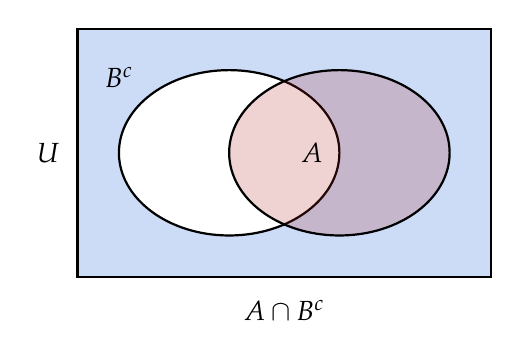
\begin{tikzpicture}[scale=0.7]
\filldraw[fill=newblue,fill opacity=1/5,thick] (-3.75,-2.25) rectangle (3.75,2.25);
	\def\firstcircle{(0:1) ellipse (2cm and 1.5cm)};
    \def\secondcircle{(0:-1) ellipse (2cm and 1.5cm)};
\filldraw[fill=white,thick] \secondcircle;
\filldraw[fill=firebrick,fill opacity=1/5,thick] \firstcircle;
\node at (0:0.5)    {$A$};
\node[above,yshift=2em] at (0:-3)    {$B^c$};
\node[left,xshift=-3pt] at (-3.75,0){$U$};
\node[below,yshift=-5pt] at (0,-2.25){$A \cap B^c$};
\end{tikzpicture}\]
\end{minipage}\hspace*{-1em}$=$\hspace*{-1em}
\begin{minipage}{0.5\textwidth}
\[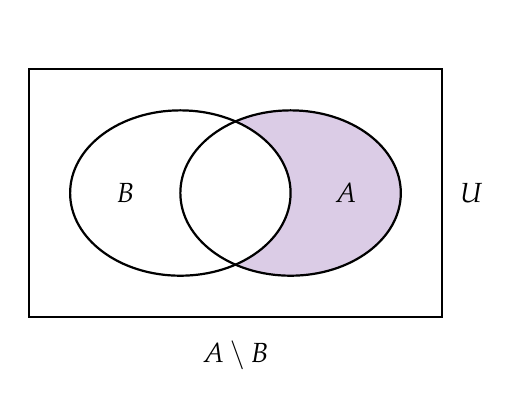
\begin{tikzpicture}[scale=0.7]
	\def\firstcircle{(0:1) ellipse (2cm and 1.5cm)};
    \def\secondcircle{(0:-1) ellipse (2cm and 1.5cm)};
    	\begin{scope}[even odd rule]
    		\clip \secondcircle (-2,-2) rectangle (3,3);
    		\fill[indigo,opacity=1/5] \firstcircle;
	\end{scope}
\draw[thick] \firstcircle;
\draw[thick] \secondcircle;
\node at ( 0:2)    {$A$};
\node at (0:-2)    {$B$};
\draw[thick] (-3.75,-2.25) rectangle (3.75,2.25);
\node[right,xshift=3pt] at (3.75,0){$U$};
\node[below,yshift=-5pt] at (0,-2.25){$A \setminus B$};
\end{tikzpicture}\]
\end{minipage}
Therefore $A\setminus B = A \cap B^c$, as noted by the Venn diagram above. 
\end{proof}

\item[(2)] Show that $A \cup B = A$ if and only if $B \subseteq A$.\\
\begin{subproof}
\begin{proof}[Scratch Notes]\hfill
\renewcommand{\qed}{}
\begin{itemize}
\item[(a)] Since we are being asked to prove an ``if and only if'' statement, that is, a biconditional payment, we need to prove two things:
\begin{align*}
&\text{if $A \cap B = A$, then $B \subseteq A$}
&\text{if $B \subseteq A$, then $A \cap B = A$}
\end{align*}
\item[(b)] To show set equality $X = Y$, we need to show two inclusions: $X \subseteq Y$ and $Y \subseteq X$. 
\item[(c)] To show set inclusion $U \subseteq V$ is equivalent to showing that
\[\text{if $x \in U$, then $x \in V$}\]
\end{itemize}
\end{proof}
\end{subproof}

\begin{proof}
First we show that if $A \cup B = A$, then $B \subseteq A$. Let us consider an arbitrary $x \in B$. Since $B \subseteq A \cup B$, we therefore also have $x \in A \cup B$. By hypothesis $A \cup B = A$, and hence $x \in A$. Thus, $B \subseteq A$. \\
\\
Let us now show that if $B \subseteq A$, then $A \cup B = A$. For this, we need to show (i) $A \subseteq A \cup B$; and (ii) $A \cup B \subseteq A$. Note that we have (i) for free, we really need to only show (ii). Let us consider an arbitrary $x \in A \cup B$. Then $x \in A$ or $x \in B$. If $x \in A$, then we have nothing to show since $x \in A$ already. Now, if $x \in B$, then since we have our hypothesis $B \subseteq A$, we also have $x \in A$. So, in the both cases $x \in A$. Thus, we have proven that $A \cup B \subseteq A$.\\
\\
This completes the proof. 
\end{proof}

\begin{proof}[Another Proof using Set Inclusion Arguments]
We first prove $A \cup B = A$ implies $B \subseteq A$, this follows immediately as
\[B \subseteq A\cup B = A.\]
Therefore $B \subseteq A$.\\
\\
Let us now prove the converse: $B \subseteq A$ implies $A \cup B = A$. As noted previously, we already have $A \subseteq A \cup B$. For the other inclusion, note that since $B \subseteq A$, we have
\[A \cup B \subseteq A \cup A = A;\]
and so $A \cup B \subseteq A$. Hence $A \cup B = A$.
\end{proof}
\end{itemize}
\end{example}

\vspace*{2em}

\begin{mdframed}
\begin{center}
{\Large Set Operations}
\end{center}
\end{mdframed}

\begin{proposition}[Set Operation Laws]
Let $A,\,B,\,C$ be sets, then
\begin{itemize}
\item Distributive Laws
\begin{align*}
\text{\emph{(a)}}\quad A\, {\color{newblue}\cup}\, (B\, {\color{firebrick}\cap}\, C) &= (A\, {\color{newblue}\cup}\, B)\, {\color{firebrick}\cap}\, (A\, {\color{newblue}\cup}\, C)\\[0.5em]
\text{\emph{(b)}}\quad A\, {\color{firebrick}\cap}\, (B\, {\color{newblue}\cup}\, C) &= (A\, {\color{firebrick}\cap}\, B)\, {\color{newblue}\cup}\, (A\, {\color{firebrick}\cap}\, C)
\end{align*}

\item De Morgan's Laws
\begin{align*}
\text{\emph{(a)}}\quad (A \cup B)^c &= A^c \cap B^c\\[0.5em]
\text{\emph{(b)}}\quad (A \cap B)^c &= A^c \cup B^c
\end{align*}
\end{itemize}
\end{proposition}
\begin{proof}
One can prove these laws either using Venn diagrams or element-wise arguments. We leave the proof to the reader.
\end{proof}

\vspace*{1em}

\begin{example}
Show $(A \setminus B) \cap (A \setminus C) = A \setminus (B \cup C)$
\begin{proof} \emph{Method 1.} Using Venn Diagrams (gets messier as we involve more sets).
\item[] \emph{Method 2.} Using set operations
\begin{align*}
(A \setminus B) \cap (A \setminus C) &= (A \cap B^c) \cap (A \cap C^c) && \text{by Proposition \ref{prop:set-id} (1), or Example \ref{example:set-proof} (1)}\\[0.5em]
 &= (A \cap A) \cap (B^c \cap C^c)\\[0.5em]
 &= A \cap (B^c \cap C^c)\\[0.5em]
 &= A \cap (B \cup C)^c && \text{by De Morgan's Laws}\\[0.5em]
 &= A \setminus (B \cup C) && \text{by Proposition \ref{prop:set-id} (1), or Example \ref{example:set-proof} (1)}
\end{align*}
This completes the proof.
\end{proof}
\end{example}
\newpage

\section{Methods of Proof II. Counterexamples, Proof by Contradiction and Existence Proofs}
\begin{mdframed}
\begin{center}
{\Large Counterexamples}
\end{center}
\end{mdframed}

\begin{discussion}
Our purpose is always to determine the truth value of statements. Consider a universally quantified statement 
\[\forall x\in S,\ R(x)\]
Is this true or false?
\item[] If you think it is true, \emph{prove it}.
\item[] If you think it is false, then its negation
\[\exists x \in S,\ \neg R(x)\]
is true. Therefore to show falsehood, we need to exhibit an (at least one) element $x_0 \in S$ such that $R(x_0)$ is false (that is, $\neg R(x_0)$ is true). $x_0$ is the called a \emph{counterexample} to the given statement. Counterexamples prove falsehood of, disproving, universally quantified statements.
\end{discussion}

\vspace*{1em}

\begin{example}
The reader has shown in an assignment that if $n$ is a sum of two squares, then
\[n \equiv 0,1,2 \modar{4}\]
Consider the converse: For an integer $n$, if $n \equiv 0,1,2 \modar{4}$, then $n$ a sum of two squares.
\end{example}
\begin{proof}[Question]
\renewcommand{\qed}{}
True or False? Probably false, so we seek a counterexample. We check the statement for small non-negative integers, in hopes of encountering a counterexample.\\[0.5em]
Since $n \equiv 0,1,2 \modar{4}$, our list is
\begin{center}
{\renewcommand{\arraystretch}{2}%
\begin{tabular}{c|cccccccccc}
$n$ & $0$ & $1$ & $2$ & $4$ & $5$ & $6$ & $8$ & $9$ & $10$ & $\cdots$\\
\hline
\makecell{sum of\\ squares} & $0^2 + 0^2$ & $0^2 + 1^2$ & $1^2 + 1^2$ & $0^2 + 2^2$ & $1^2 + 2^2$ & {\color{firebrick}No.} & \phantom{$1^2 +$} & \phantom{$1^2 +$} & \phantom{$1^2 +$} & 
\end{tabular}
}
\end{center}
\end{proof}
\begin{proof}[Answer]
False. Since $6 \equiv 2 \modar{4}$, but it is not a sum of two squares. 
\end{proof}

\vspace*{1em}

\begin{example}
True or False?
\item[] Let $a,b \in \rr$ such that $a,b \neq 0$. For all $x,y \in \rr_{>0}$, is
\[\frac{a^2}{2b^2}\,x^2 + \frac{b^2}{2a^2}\,y^2 > xy\]
\end{example}
\begin{proof}[Scratch Notes]
\renewcommand{\qed}{}
We will try and prove it. If the proof goes through, the statement true and we have a proof. If the proof does not go through, then the reason why it did not could possibly give us a way to produce a counterexample.\newpage
\begin{align*}
\mathrm{L.H.S.} - \mathrm{R.H.S.} &= \frac{a^2}{2b^2}\,x^2 + \frac{b^2}{2a^2}\,y^2 - xy\\[0.5em]
 &= \frac{1}{2}\left(\frac{a^2}{b^2}\,x^2 - 2xy + \frac{b^2}{a^2}\,y^2\right)\\[0.5em]
 &= \frac{1}{2}\left(\left(\frac{ax}{b}\right)^2 - 2\left(\frac{ax}{b}\right)\left(\frac{by}{a}\right) + \left(\frac{by}{a}\right)^2\right)\\[0.5em]
 &= \frac{1}{2}\left(\frac{ax}{b} - \frac{by}{a}\right)^2 \geq 0
\end{align*}
So, when do we get the above expression $=0$? Exactly when
\[\frac{ax}{b} = \frac{by}{a}\]
Do such $x$ and $y$ exist? Well yes, consider $x = b^2$ and $y = a^2$, then
\[\frac{ax}{b} = ab = ba = \frac{by}{a}\]
\end{proof}
\begin{proof}[Answer]
False. Let $x = b^2$ and $y = a^2$. Then
\begin{align*}
\mathrm{L.H.S.} &= \frac{a^2}{2b^2}\,x^2 + \frac{b^2}{2a^2}\,y^2\\[0.5em]
 &= \frac{a^2}{2b^2}\cdot (b^2)^2 + \frac{b^2}{2a^2}\cdot (a^2)^2\\[0.5em]
 &= \frac{a^2b^2}{2} + \frac{b^2a^2}{2}\\[0.5em]
 &= a^2b^2\\[1em]
\mathrm{R.H.S.} &= xy\\[0.5em]
 &= a^2b^2
\end{align*}
So, $\mathrm{L.H.S.} = \mathrm{R.H.S.}$, and therefore $\mathrm{L.H.S.} > \mathrm{R.H.S.}$ does not hold.
\end{proof}

\vspace*{2em}

\begin{mdframed}
\begin{center}
{\Large Proof by Contradiction}
\end{center}
\end{mdframed}

\begin{discussion}
Let $R$ be a statement. What is a \cdef{proof\ by\ contradiction}? The method is as follows: to show $R$ is true, show that the negation of $R$ leads to a contradiction $\bot$. Logical structure,
\[R \equiv (\neg R \implies \bot)\]
\begin{center}
{\renewcommand{\arraystretch}{1.5}%
\begin{tabular}{|>{\centering}m{1cm}|>{\centering}m{1cm}|>{\centering}m{1cm}|>{\centering\arraybackslash}m{1.5cm}|}
\hline
\rowcolor{lightgrey}
$R$ & $\neg R$ & $\bot$ & $\neg R \implies \bot$ \\
\hline
$\true$ & $\false$ & $\false$ & $\true$\\
\hline
$\false$ & $\true$ & $\false$ & $\false$\\
\hline
\end{tabular}
}
\end{center}
If the negation of $R$ gives us a contradiction, that is, if $(\neg R \implies \bot)$ is true, since the conclusion $\bot$ is always false, the only possibility is for the hypothesis $\neg R$ to be also false. Hence $R$ is true.\\
\\
{\bf Special but useful case.} If $R$ is of the form $P \implies Q$, then to prove $P \implies Q$ we prove the following
\[\neg(P \implies Q) \implies \bot\]
Recall that \[\neg(P \implies Q) \equiv \neg(\neg P \vee Q) \equiv P \wedge \neg Q.\] Thus, to prove $P \implies Q$, show that
\[(P \wedge \neg Q) \implies \bot\]
The contradiction we often try to find is $S \wedge \neg S$ for some statement $S$. In other words, assume $P$ is true and also assume the conclusion $Q$ is false, then we try to find a contradiction $S \wedge \neg S$, finding an appropriate $S$ is the heart of the proof.
\end{discussion}

\vspace*{1em}

\begin{example}
Suppose an integer $m$ is such that $2\mid m$ but $4\nmid m$. Show that there are no integer solutions $x,y$ to the equation
\[x^2 + 2y^2 = m\]
This is a \emph{non-existence statement}, we use proof by contradiction to prove such statements.
\end{example}
\begin{proof}[Scratch Notes for Proof]\renewcommand{\qed}{}
Suppose we have an integer $m$ is such that $2\mid m$ but $4\nmid m$, therefore $m \equiv 2\modar{4}$. The logical structure of the statement is
\begin{align*}
\text{Hypothesis } & P(m): m \equiv 2 \modar{4}\\[0.5em]
\text{Conclusion } & Q(m): x^2 + 3y^2 = m \text{ has no integer solution }x,y
\end{align*}
We need to show \[\forall m \in \zz,\ P(m) \implies Q(m)\]
To give a proof by contradiction, we assume two things: $P(m)$ and $\neg Q(m)$. That is, suppose $m \equiv 2\modar{4}$ and that there exist integers $x,y$ such that $x^2 + 3y^2 = m$.\\
\\
How do we find a contradiction? Consider integers modulo $4$, we have seen that for any integer $n$, we have $n^2 \equiv 0,1\modar{4}$. So, for the solutions $x,y$, we have $x^2 \equiv 0,1\modar{3}$ and $y^2 \equiv 0,1\modar{3}$. So, we have the cases
\begin{align*}
x^2 \equiv 0 \modar{4},&\; y^2 \equiv 0 \modar{4} & \text{So, } x^2 + 3y^2 &\equiv 0 \modar{4}\\[0.5em]
x^2 \equiv 1 \modar{4},&\; y^2 \equiv 0 \modar{4} & \text{So, } x^2 + 3y^2 &\equiv 1 \modar{4}\\[0.5em]
x^2 \equiv 0 \modar{4},&\; y^2 \equiv 1 \modar{4} & \text{So, } x^2 + 3y^2 &\equiv 3 \modar{4}\\[0.5em]
x^2 \equiv 1 \modar{4},&\; y^2 \equiv 1 \modar{4} & \text{So, } x^2 + 3y^2 &\equiv 4 \equiv 0 \modar{4}
\end{align*}
Thus, $x^2 + 3y^2 \equiv 0,1,3 \modar{4}$ and therefore $x^2 + 3y^2 \not\equiv 2 \modar{3}$. But our assumption is $x^2 + 3y^2 = m \equiv 2 \modar{4}$, this our $S$. Hence, we have arrived at a contradiction. So, $x^2 + 3y^2 = m$ cannot have integer solutions. 
\end{proof}
\begin{proof}
Check back tomorrow for a proof.
\end{proof}

%\vspace*{1em}

\begin{discussion}
We now have three methods to prove implications $P \implies Q$
\begin{center}
\begin{tabular}{>{\centering}m{1.75cm} >{\centering}m{0.5cm} >{\centering}m{2cm} >{\centering}m{0.5cm} >{\centering\arraybackslash}m{2.75cm}}
$P \implies Q$ & $\equiv$ & $\neg Q \implies \neg P$ & $\equiv$ & $(P \wedge \neg Q) \implies \bot$\\
{\scriptsize(I) Direct Proof} && {\scriptsize(II) Proof by Contrapositive} && {\scriptsize(III) Proof by Contradiction}\\
\end{tabular}
\end{center}
\end{discussion}

\vspace*{1em}

\begin{example}
Let $x \in \rr$ and $x \neq 0$. Show that if $x + \dfrac{1}{x} < 2$, then $x > 0$.
\end{example}
\begin{proof}[Direct Proof]
Suppose $x$ is a non-zero real number such that $x + 1/x < 2$, we show $x < 0$. We first observe that we have
\[x + \frac{1}{x} - 2 < 0\]
Note that
\begin{align*}
x + \frac{1}{x} - 2 &= \frac{x^2 + 1 - 2x}{x}\\[0.5em]
&= \frac{(x-1)^2}{x}
\end{align*}
Since $(x - 1)^2 \geq 0$ for any $x$, for the ration to be negative, we necessarily must have $x< 0$. This completes the proof.
\end{proof}
\vspace*{0.2em}
\begin{proof}[Proof by Contrapositive]
We prove its contrapositive. Assume $x \geq 0$, since $x\neq 0$, we may assume $x > 0$. We wish to prove $x + 1/x \geq 2$. Using AM $\geq$ GM, we have
\[\frac{1}{2}\left(x + \frac{1}{x}\right) \geq \sqrt{x\cdot \frac{1}{x}} = 1\]
Hence $x + \dfrac{1}{x} \geq 2$. This completes the proof.
\end{proof}
\vspace*{0.2em}
\begin{proof}[Proof by Contrapositive]
For the sake of contradiction, assume that $x \geq 0$ is a real number such that $x + 1/x < 2$ and $x > 0$. Using AM $\geq$ GM, we have
\[\frac{1}{2}\left(x + \frac{1}{x}\right) \geq \sqrt{x\cdot \frac{1}{x}} = 1\]
Hence $x + \dfrac{1}{x} \geq 2$. This contradicts our hypothesis, hence $x + 1/x < 2$ implies $x < 0$.
\end{proof}

%\vspace*{2em}

\begin{mdframed}
\begin{center}
{\Large Existence Proofs}
\end{center}
\end{mdframed}

\begin{discussion}
We now turn our attention to proving 
\[\exists x \in S,\ R(x)\]
\emph{there exists an $x$ such that $R(x)$ is true.} Methods to prove existence results
\begin{itemize}
\item[(1)] Exhibit $x \in S$ satisfying $R(x)$.
\item[(2)] Use other existence theorems.
\item[(3)] Use proof by contradiction. \emph{the method of choice for proving existence results}.
\end{itemize}
\end{discussion}

\vspace*{1em}

\begin{example}\hfill
\begin{itemize}[itemsep=1em,leftmargin=4em]
\item[for (1)] Rationality of $a^b$, where $a,b \in \rr$ and $a,b > 0$.
\begin{proof}[Question]\renewcommand{\qed}{}
Is $a^b$ is rational or irrational?
\end{proof}
\begin{proof}
We divide this into cases: where $a$ and $b$ are rational or irrational.
\begin{itemize}[leftmargin=4em]
\item[Case I.] $a$ is rational, $b$ is rational
\begin{align*}
2^3 &= 8 \text{ (rational)}\\
2^{1/2} &= \sqrt{2} \text{ (irrational)}
\end{align*}

\item[Case II.] $a$ is rational, $b$ is irrational
\begin{align*}
1^{\sqrt{2}} &= 1 \text{ (rational)}\\
2^{\log_23} &= 3 \text{ (rational)}\\
2^{\log_2 \sqrt{3}} &= \sqrt{3} \text{ (irrational)}
\end{align*}

\item[Case III.] $a$ is irrational, $b$ is rational
\begin{align*}
(\sqrt{2})^2 &= 2 \text{ (rational)}\\
(\sqrt{2})^3 &= 2\sqrt{2} \text{ (irrational)}
\end{align*}

\item[Case IV.] $a$ is irrational, $b$ is irrational
\begin{align*}
(\sqrt{2})^{2\log_2 3} = 2^{\log_2 3} &= 3 \text{ (rational)}\\
(\sqrt{2})^{\log_2 3} = (2^{\log_2 3})^{1/2} &= \sqrt{3} \text{ (irrational)}
\end{align*}
\end{itemize}
\end{proof}

\item[for (2)] Show that $x^2 + 2x - 5 = 0$ has a solution in the interval $[1,2]$.
\begin{proof}
We use the following existence result to prove this.
\begin{theorem}[Intermediate Value Theorem]
Suppose $f:[a,b] \to \rr$ is continuous. If $f(a) < 0$ and $f(b) > 0$, then there exists a $c \in (a,b)$ such that $f(c) = 0$.
\end{theorem}
Back to our proof. As a polynomial $f(x) = x^2 + 2x - 5$ is continuous. Since $f(1) = -2 < 0$ and $f(2) = 3 > 0$, therefore there exists a $c \in (1,2)$ such that $f(c) = 0$. That is, $c^2 + 2c - 5 = 0$. This completes our proof.
\end{proof}

\item[for (3)] We look at a very fundamental counting principle.
\begin{theorem}[Pigeonhole Principle]
Suppose $n$ objects are placed in $m$ boxes. If $n > m$, then there exists a box containing at least two objects. 
\end{theorem}\vspace*{-1em}
\begin{proof}
For the sake of contradiction, suppose $n > m$ and every box contains at most one object. Since there are $m$ boxes, it follows that there are at most $m$ objects; that is $n \leq m$. This contradicts our hypothesis that $n > m$. This completes our proof.
\end{proof}
\end{itemize}
\end{example}

\vspace*{1em}

\begin{example}[on the Pigeonhole Principle]
Let $S$ be a set of three integers. For a non-empty subset $A$ of $S$, let $\sigma_A$ be the sum of elements in $A$. Prove that there exist two distinct nonempty subsets $B$ and $C$ of $S$ such that $\sigma_B \equiv \sigma_C \modar{6}$.
\end{example}

\begin{proof}[Experiments]\renewcommand{\qed}{}
Let $S = \set{2,5,7}$
\begin{center}
{\renewcommand{\arraystretch}{1.5}%>{\columncolor[gray]{0.8}}
\begin{tabular}{c|>{\columncolor{newblue!20}}c|c|>{\columncolor{firebrick!20}}c|>{\columncolor{firebrick!20}}c|c|c|>{\columncolor{newblue!20}}c|}
%\begin{tabular}{c|>{\columncolor[red]{0.8}}cc>{\columncolor[blue]{0.8}}c>{\columncolor[blue]{0.8}}ccc>{\columncolor[red]{0.8}}c}
$A$ & $\set{2}$ & $\set{5}$ & $\set{7}$ & $\set{2,5}$ & $\set{5,7}$ & $\set{7,2}$ & $\set{2,5,7}$\\
\hline
$\sigma_A$ & $2$ & $5$ & $7$ & $7$ & $11$ & $9$ & $14$
\end{tabular}
}
\end{center}
Subsets $B = \set{2},\ \sigma_B = 2$ and $C = \set{2,5,7},\ \sigma_C = 14$ are such that $\sigma_{B} \equiv \sigma_{C} \modar{6}$. Also, subsets $B' = \set{7},\ \sigma_{B'} = 7$ and $C' = \set{2,5},\ \sigma_{C'} = 7$ are such that $\sigma_{B'} \equiv \sigma_{C'} \modar{6}$.\\
\\
Let $S = \set{1,3,8}$
\begin{center}
{\renewcommand{\arraystretch}{1.5}%
\begin{tabular}{c|c|>{\columncolor{forest!20}}c|c|c|c|>{\columncolor{forest!20}}c|c}
$A$ & $\set{1}$ & $\set{3}$ & $\set{8}$ & $\set{1,3}$ & $\set{3,8}$ & $\set{8,1}$ & $\set{1,3,8}$\\
\hline
$\sigma_A$ & $1$ & $3$ & $8$ & $4$ & $11$ & $9$ & $12$
\end{tabular}
}
\end{center}
Subsets $B = \set{3},\ \sigma_B = 3$ and $C = \set{1,8},\ \sigma_C = 9$ are such that $\sigma_{B} \equiv \sigma_{C} \modar{6}$.
\end{proof}

\begin{proof}
Let $S$ be a three element set. The number of non-empty subsets of $S$ are $\abs{\cat{P}(S)} - 1 = 2^3 - 1 = 7$. So, we obtain $n = 7$ integers $\sigma_A$ for every non-empty subset $A$ of $S$. These are our objects. While there are $m = 6$ possibly remainders when an integer is divided by $6$. These are our boxes.

\begin{center}
\begin{tabular}{cccccccccccccc}
$\sigma_A$ & $\bullet$ && $\bullet$ && $\bullet$ && $\bullet$ && $\bullet$ && $\bullet$ && $\bullet$\\[1em]
remainders && $\underset{0}{\fbox{\phantom{11}}}$ && $\underset{1}{\fbox{\phantom{11}}}$ && $\underset{2}{\fbox{\phantom{11}}}$ && $\underset{3}{\fbox{\phantom{11}}}$ && $\underset{4}{\fbox{\phantom{11}}}$ && $\underset{5}{\fbox{\phantom{11}}}$
\end{tabular}
\end{center}

Therefore, by the Pigeonhole Principle, there must be one box with at least two objects; that is, there must exist two sets $B$ and $C$ such that $\sigma_B$ and $\sigma_C$ leave the same remainder when divided by $6$ (are in the same box). This completes the proof. 
\end{proof}

\vspace*{1em}

\begin{discussion}
Previously we discussed existence proofs, that is, proving a statement of the form
\[\exists x \in S,\ R(x)\]
We wish to now discuss a proof of a variation about the above statement. Recall that the above statement says \emph{there exists an $x \in S$ such that $R(x)$ is true}. We focus on a statement when such an $x$ is unique, that is, not only is $R(x)$ true for this $x$, $x$ is the only element for which $R(x)$ is true. The statement is then \emph{there exists a unique $x \in S$ such that $R(x)$ is true}, and is denoted symbolically as
\[\exists ! x \in S,\ R(x)\]
So, there are two steps to proving such a statement
\begin{itemize}
\item[] Step 1. Existence proof. Prove such an $x$ exists.
\item[] Step 2. Uniqueness proof. Prove such an $x$ is unique.
\end{itemize}
We have already discussed Step 1. For Step 2., one typically does the following
\begin{itemize}
\item[(1)] If $x,y \in S$ are such that $R(x)$ and $R(y)$ is true, prove that $y = x$.
\item[(2)] If $x,y \in S$ are such that $R(x)$ and $R(y)$ is true and $y \neq x$, then show that this leads to a contradiction.
\end{itemize}
\end{discussion}

\vspace*{1em}

\begin{example}\label{example:lec13-ex1}
Show that $x^5 + 2x - 5 = 0$ has a unique root between $x = 1$ and $x = 2$.
\end{example}
\begin{proof}
We are being asked to prove both an existence statement and a uniqueness statement.
\item[] (Existence)
Let $f(x) = x^5 + 2x - 5$. Since $f(1) = -2 < 0$ and $f(2) = 31 > 0$, by the Intermediate Value Theorem, there exists a real number $c \in (1,2)$ such that $f(c) = 0$.\\
\item[] (Uniqueness, Method 1)
Suppose there exist $c_1,c_2 \in (1,2)$ such that $f(c_1) = f(c_2) = 0$. We aim to show $c_1 = c_2$. By assumption,
\[c_1^5 + 2c_1 - 5 = f(c_1) = 0 \quad \text{and} \quad c_2^5 + 2c_2 - 5 = f(c_2) = 0\]
Taking their difference of these two equations, we obtain
\[(c_1^5 - c_2^5) + 2(c_1 - c_2) = 0\tag{$*$}\]
\begin{subproof}
To show $c_1 = c_2$, we want to factor out $c_1 - c_2$ from the L.H.S. in ($*$). We use the following identity: for any real numbers $x,y$
\[x^n - y^n = (x-y)(x^{n-1} + x^{n-2}y + \cdots + xy^{n-2} + y^{n-1})\]
\end{subproof}
\vspace*{0.5em}
Factoring out $c_1 - c_2$ from the L.H.S. in ($*$), we get
\[(c_1 - c_2)(c_1^4 + c_1^3c_2 + c_1^2c_2^2 + c_1c_2^3 + c_2^4 + 2) = 0\]
\begin{subproof}
To show $c_1 = c_2$, we want to argue that the other factor $c_1^4 + c_1^3c_2 + c_1^2c_2^2 + c_1c_2^3 + c_2^4 + 2$ is non-zero.
\end{subproof}
\vspace*{0.5em}
Since $1<c_1,c_2 < 2$, we have $c_1^4,\,c_1^3c_2,\,c_1^2c_2^2,\,c_1c_2^3,\,c_2^4 > 1$. Thus, we get 
\[c_1^4 + c_1^3c_2 + c_1^2c_2^2 + c_1c_2^3 + c_2^4 + 2 > 7\]
In particular, this factor is non-zero. Hence, necessarily $c_1 - c_2 = 0$. This completes the uniqueness proof.\\
\item[] (Uniqueness, Method 2) Suppose there exist $c_1,c_2 \in (1,2)$ such that $f(c_1) = f(c_2) = 0$ and $c_1 \neq c_2$. We will provide a contradiction. Since $f(x) = x^5 + 2x - 5$, we have 
\[f'(x) = 5x^4 + 2 > 0.\]
Therefore $f(x)$ is a strictly increasing function. We may assume, without loss of generality, that $c_1 < c_2$. Then, since $f$ is increasing, we have $f(c_1) < f(c_2)$. This contradicts our assumption that $f(c_1) = f(c_2) = 0$. Hence, necessarily $c_1 = c_2$. This completes the uniqueness proof.
\end{proof}

\vspace*{1em}

\begin{remark}
Generally speaking, proof by contradiction is the method of choice for existence and uniqueness proofs. But if you can give a direct proof, by all means do so.
\end{remark}

\vspace*{2em}

\begin{mdframed}
\begin{center}
{\Large Disproving Existence Statements}
\end{center}
\end{mdframed}

\begin{discussion}
To disprove
\[\exists x \in S,\ R(x)\]
Prove that its negation is true
\[\neg(\exists x \in S,\ R(x)) \equiv \forall x \in S,\ \neg R(x)\]
\end{discussion}

\vspace*{1em}

\begin{example}
Disprove that there exist integers $a \geq 2$ and $n \geq 1$ such that
\[a^2 + 1 = 2^n\]
\end{example}
\begin{proof}
We prove that for all integers $a \geq 2$ and $n \geq 1$, we have $a^2 + 1 \neq 2^n$, by using proof by contradiction. Suppose there exist $a \geq 2$ and $n \geq 1$ such that $a^2 + 1 = 2^n$.\\[0.5em]
Since $n \geq 1$, $2^n$ is even. Therefore $a^2$ is odd, and hence so is $a$. We may then write $a = 2k + 1$ for an integer $k$. Since $a \geq 2$, we get that $k \geq 1$. Therefore,
\begin{align*}
a^2 + 1 &= (2k + 1)^2 + 1\\[0.5em]
&= (4k^2 + 4k + 1) + 1\\[0.5em]
&= 4k^2 + 4k + 2\\[0.5em]
&= 2(2k^2 + 2k + 1)
\end{align*}
Since $a^2 + 1 = 2^n$, by assumption, we have $2(2k^2 + 2k + 1) = 2^n$. Hence,
\[2^{n-1} = 2k^2 + 2k + 1 = 2k(k+1) + 1\]
Which gives us
\[2k(k + 1) = 2^{n-1} - 1\]
Since $k \geq 1$, the L.H.S. $\geq 4$. Thus $2^{n-1} - 1 \geq 4$, and hence necessarily $n > 1$. Therefore the R.H.S., $2^{n - 1} - 1$ is odd, but the L.H.S. is always even. We have thus arrived at a contradiction. This completes the proof.
\end{proof}
\newpage

\section{Principle of Mathematical Induction}
\vspace*{1em}

\begin{discussion}
We have the set of positive integers
\[\zz_{>0} = \set{1,2,3,\ldots}\]
The principle of mathematical induction is a method of proof for statements of the form
\[\forall n \in \zz_{>0},\ P(n)\]
\[\text{$P(1)$ is true, and $P(2)$ is true, and $P(3)$ is true, and $\ldots$}\]
\[\text{and $P(n)$ is true, and $P(n+1)$ is true, and $\ldots$}\]
To prove such a statement, do the following
\begin{itemize}[leftmargin=4em]
\item[Step 1.] (\emph{Base Step}, or \emph{Initial Step}) Prove that $P(1)$ is true.
\item[Step 2.] (\emph{Inductive Step}) Prove that for all $k \geq 1,\ P(k)$ implies $P(k + 1)$. That is, prove 
\[\forall k \in \zz_{>0},\ P(k) \implies P(k+1)\]
In words, assume $P(k)$ is true (\emph{inductive hypothesis}) and conclude $P(k+1)$ is true for any $k \geq 1$.
\end{itemize}
This is the {\color{blue}(first)} \cdef{principle\ of\ mathematical\ induction}.\\
\\
What are we doing?
\[\begin{tikzcd}
\underset{\text{(Step 1)}}{\text{$P(1)$ is true}} \arrow[r, "{\text{\scriptsize for $k=1$}}"',draw=none]\arrow[r, "\text{Step 2}"] & \text{$P(2)$ is true} \arrow[r, "{\text{\scriptsize for $k=2$}}"',draw=none]\arrow[r, "\text{Step 2}"] & \text{$P(3)$ is true}  \arrow[r, "{\text{\scriptsize for $k=3$}}"',draw=none]\arrow[r, "\text{Step 2}"] &       \cdots \\
\cdots  \arrow[r, "{\text{\scriptsize for $k=n-1$}}"',draw=none]\arrow[r, "\text{Step 2}"]  & \text{$P(n)$ is true} \arrow[r, "{\text{\scriptsize for $k=n$}}"',draw=none]\arrow[r, "\text{Step 2}"] & \text{$P(n+1)$ is true} \arrow[r] & \cdots
\end{tikzcd}\]
The logical foundation is the fact that the statement \[P \land (P \implies Q) \implies Q\] is a tautology. So, if $P(k)$ is true and $P(k) \implies P(k+1)$ is true, then $P(k+1)$ is true. 
\end{discussion}

%\vspace*{1em}

\begin{example}
Show that for $n \geq 1$,
\[1 + 2 + \cdots + n = \frac{n(n+1)}{2}\]
\end{example}
\begin{proof}
We have the open sentence
\[P(n):1 + 2 + \cdots + n = \frac{n(n+1)}{2}\]
We give a proof to the statement \emph{for all $n \geq 1,\ P(n)$ is true} using the principle of mathematical induction.
\item[] (Base Step, $n = 1$) Consider the statement $P(1)$. L.H.S. $ = 1$, while
\[\mathrm{R.H.S.} = \frac{1(1 + 1)}{2} = \frac{2}{2} = 1\]
Therefore $P(1)$ is true.\\
\item[] (Inductive Step) Assume $P(k)$ is true, that is,
\[1 + 2 + \cdots + k = \frac{k(k+1)}{2}\]
We wish to prove $P(k+1)$ is true, that is, we wish to prove the following equality
\begin{align*}
1 + 2 + \cdots + (k + 1) &= \frac{(k+1)((k+1)+1)}{2}\\[1em]
 &= \frac{(k+1)(k+2)}{2}
\end{align*}
is true.\\[0.5em]
Note,
\begin{align*}
1 + 2 + \cdots + (k + 1) &= 1 + 2 + \cdots + k + (k + 1)\\[0.5em]
 &= \frac{k(k+1)}{2} + (k+1) && \text{by the inductive hypothesis}\\[0.5em]
 &= (k+1)\left(\frac{k}{2} + 1\right)\\[0.5em]
 &= \frac{(k+1)(k+2)}{2}
\end{align*}
Therefore $P(k+1)$ is true.\\
\\
Hence, by the principle of mathematical induction, $P(n)$ is true for every integer $n \geq 1$.
\end{proof}

\vspace*{1em}

\begin{discussion}
It happens often that our base case for a statement $P(n)$, that is the first instance for which $P(n)$ is true, does not occur at $n = 1$, but may occur for a larger integer, say some $n = m$. We may still use the principle of mathematical induction by ``starting induction from $n = m$''. One then proves 
\begin{itemize}
\item[](Base Case) Prove $P(m)$ is true.
\item[](Inductive Step) For any $k \geq m$, prove $P(k) \implies P(k+1)$ is true. 
\end{itemize}
This is the {\color{blue}(second)} \cdef{principle\ of\ mathematical\ induction}.
\end{discussion}

\vspace*{1em}

\begin{example}
Show that for $n \geq 5$, we have $2^n > n^2$.
\end{example}
\begin{proof}[Experiment]
\renewcommand{\qed}{}\hfill
\begin{center}
{\renewcommand{\arraystretch}{1.5}%
\begin{tabular}{c|cccc|>{\columncolor{newblue!30}}c>{\columncolor{newblue!20}}c>{\columncolor{newblue!20}}c>{\columncolor{newblue!20}}c}
$n$ & $1$ & $2$ & $3$ & $4$ & $5$ & $6$ & $7$ & $\cdots$\\
\hline
$2^n$ & $2$ & $4$ & $8$ & $16$ & $32$ & $64$ & $128$ & $\cdots$\\
$n^2$ & $1$ & $4$ & $9$ & $16$ & $25$ & $36$ & $49$ & $\cdots$\\
\end{tabular}
}
\end{center}
\end{proof}
\begin{proof}
We have the open sentence
\[P(n):2^n = n^2\]
We give a proof to the statement \emph{for all $n \geq 5,\ P(n)$ is true} using the principle of mathematical induction.
\item[] (Base Step, $n = 5$) Consider the statement $P(5)$. Note that
\[2^5 = 32 > 25 = 5^2\]
Therefore $P(1)$ is true.\\
\item[] (Inductive Step) Assume $P(k)$ is true for some $k \geq 5$, that is, $2^k > k^2$. We wish to prove $P(k+1)$ is true, that is, we wish to prove $2^{k+1} > (k+1)^2$ is true.\\[0.5em]
Note,
\begin{align*}
2^{k+1} - (k+1)^2 &= 2\cdot 2^k - (k + 1)^2\\[0.5em]
 &> 2\cdot k^2 - (k + 1)^2 && \text{by the inductive hypothesis}\\[0.5em]
 &= 2k^2 - (k^2 + 2k + 1)\\[0.5em]
 &= k^2 - 2k - 1\\[0.5em]
 &= k^2 - 2k + 1 - 2\\[0.5em]
 &= (k - 1)^2 - 2\\[0.5em]
 &> 0 && \text{for any $k \geq 5$}
\end{align*}
Therefore $P(k+1)$ is true.\\
\\
Hence, by the principle of mathematical induction, $P(n)$ is true for every integer $n \geq 5$.
\end{proof}

\vspace*{1em}

\begin{example}
Show that for $n \geq 2$ and for any $a_1,\ldots,a_n \geq 0$, we have
\[(n-1)\left(\sum_{i=1}^n a_i^2 \right) \geq 2 \sum_{1\leq i < j \leq n}a_ia_j\]
\begin{itemize}[leftmargin=4em]
\item[$(n=2)$] For $a_1,a_2 \geq 0$
\[a_1^2 + a_2^2 \geq 2a_1a_2\]
\item[$(n=3)$] For $a_1,a_2,a_3 \geq 0$
\[2(a_1^2 + a_2^2 + a_3^2) \geq 2(a_1a_2 + a_2a_3 + a_1a_3)\]
\item[$(n=4)$] For $a_1,a_2,a_3,a_4 \geq 0$
\[3(a_1^2 + a_2^2 + a_3^2 + a_4^2) \geq 2(a_1a_2 + a_1a_3 + a_1a_4 + a_2a_3 + a_2a_4 + a_3a_4)\]
\end{itemize}
\end{example}
\begin{proof}
We have the open sentence
\[P(n):(n-1)\left(\sum_{i=1}^n a_i^2 \right) \geq 2 \sum_{1\leq i < j \leq n}a_ia_j,\quad a_1,\ldots,a_n \geq 0\]
We give a proof to the statement \emph{for all $n \geq 2,\ P(n)$ is true} using the principle of mathematical induction.
\item[] (Base Step, $n = 2$) Consider the statement \[P(2):a_1^2 + a_2^2 \geq 2a_1a_2,\quad a_1,a_2 \geq 0\] Note that
\begin{align*}
a_1^2 + a_2^2 - 2a_1a_2 &= (a_1)^2 - 2(a_1)(a_2) + (a_2)^2\\[0.5em]
 &= (a_1 - a_2)^2\\[0.5em]
 &\geq 0
\end{align*}
Therefore $P(2)$ is true.\\
\item[] (Inductive Step) Assume $P(k)$ is true for some $k \geq 2$, that is, \[(k-1)\left(\sum_{i=1}^k a_i^2 \right) \geq 2 \sum_{1\leq i < j \leq k}a_ia_j,\quad a_1,\ldots,a_k \geq 0.\] We wish to prove $P(k+1)$ is true, that is, we wish to prove \[k\left(\sum_{i=1}^{k+1} a_i^2 \right) \geq 2 \sum_{1\leq i < j \leq k+1}a_ia_j,\quad a_1,\ldots,a_{k+1} \geq 0\] is true. Our first step is to re-write the L.H.S. $-$ R.H.S. in such a way that we can use the inductive hypothesis $P(k)$. We observe

\begin{align*}
k\left(\sum_{i=1}^{k+1} a_i^2 \right)& - 2 \sum_{1\leq i < j \leq k+1}a_ia_j\\[1em]
 &= (k-1)\left(\sum_{i=1}^{k+1} a_i^2 \right) + \left(\sum_{i=1}^{k+1} a_i^2 \right) - 2 \sum_{1\leq i < j < k+1}a_ia_j - 2 \sum_{1\leq i < j = k+1}a_ia_j\\[1em]
 &= (k-1)\left(\sum_{i=1}^{k} a_i^2 + a_{k+1}^2 \right) + \left(\sum_{i=1}^{k+1} a_i^2 \right) - 2 \sum_{1\leq i < j \leq k}a_ia_j - 2 \sum_{1\leq i \leq k}a_ia_{k+1}\\[1em]
 &= (k-1)a_{k+1}^2 + \left(\sum_{i=1}^{k+1} a_i^2 \right) - 2 \sum_{i=1}^{k}a_ia_{k+1} + \underbrace{(k-1)\left(\sum_{i=1}^{k} a_i^2 \right)- 2 \sum_{1\leq i < j \leq k}a_ia_j}_{\text{$\geq 0$ by $P(k)$}}
\end{align*}
Therefore by our observations above and the inductive hypothesis, we have
\begin{align*}
k\left(\sum_{i=1}^{k+1} a_i^2 \right) - 2 \sum_{1\leq i < j \leq k+1}a_ia_j & \geq (k-1)a_{k+1}^2 + \left(\sum_{i=1}^{k+1} a_i^2 \right) - 2 \sum_{i=1}^{k}a_ia_{k+1}\\[1em]
 &= ka_{k+1}^2 - a_{k+1}^2 + \left(\sum_{i=1}^{k} a_i^2 + a_{k+1}^2 \right) - 2 \sum_{i=1}^{k}a_ia_{k+1} - a_{k+1}^2\\[1em]
 &= \left(\sum_{i=1}^{k} a_i^2 \right)+ka_{k+1}^2 - 2 \sum_{i=1}^{k}a_ia_{k+1}\\[1em]
 &= (a_1^2 + a_{k+1}^2 - 2a_1a_{k+1}) + (a_2^2 + a_{k+1}^2 - 2a_2a_{k+1}) \,+\\ &\qquad\cdots + (a_k^2 + a_{k+1}^2 - 2a_ka_{k+1})\\[1em]
 &= (a_1 - a_{k+1}) + (a_2 - a_{k+1})^2 + \cdots + (a_k - a_{k+1})^2 \geq 0
\end{align*}
Therefore $P(k+1)$ is true.\\
\\
Hence, by the principle of mathematical induction, $P(n)$ is true for every integer $n \geq 2$.
\end{proof}

\vspace*{1em}

\begin{example}[try it yourself!]\label{geom-sum}
Show that for $n \geq 1$ and a real number $a \neq 1$, we have
\[1 + a + \cdots + a^n = \frac{1 - a^{n+1}}{1 - a}\]
\end{example}

\vspace*{1em}

\begin{remark}
Re-writing the equality in Example \ref{geom-sum} as
\[1 - a^{n+1} = (1-a)(1 + a + \cdots + a^n), \tag{$\star$}\]
this is now true for $a = 1$ as well. So $(\star)$ is true for all real numbers $a$.\\
\\
If we write $a = y/x$ for real numbers $x,y$, we get
\[1 - (y/x)^{n+1} = (1-(y/x))(1 + (y/x) + \cdots + (y/x)^n)\]
Multiplying both sides by $x^n$, we get
\[x^{n+1} - y^{n+1} = (x - y)(x^n + x^{n-1}y + \cdots + xy^{n-1} + y^n)\]
This is the formula we used in Example \ref{example:lec13-ex1}.
\end{remark}

\vspace*{2em}

\begin{mdframed}
\begin{center}
{\Large Strong Principle of Mathematical Induction}
\end{center}
\end{mdframed}

\begin{discussion}
The \cdef{strong\ principle\ of\ mathematical\ induction} is a variation of the principle of mathematical induction. We are still trying to prove statements of the form 
\[\forall n \geq 1,\ P(n)\]
or more generally {\color{indigo}$\forall n \geq m,\ P(n)$} for some fixed integer $m$.
This time our steps are:
\begin{itemize}[leftmargin=*]
\item[](Base Case)\\[0.5em] Prove $P(1)$ is true; or more generally {\color{indigo}$P(m)$ is true.}
\item[](Inductive Step)\\[0.5em] For any $k \geq 1$, prove \[\text{$P(1)$ and $P(2)$ and $\ldots$ and $P(k)$ together imply $P(k+1)$}\] 
Or more generally, {\color{indigo} for all $k \geq m$, prove $P(m) \land P(m+1) \land \cdots \land P(k) \implies P(k+1)$ is true}.
\end{itemize}
\end{discussion}

\vspace*{1em}

\begin{theorem}[Prime Factorisation Theorem]
Every positive integer $n \geq 2$ is a product of primes
\end{theorem}
\begin{proof}
We have the open sentence
\[P(n):n \text{ is a product of primes}\]
We give a proof to the statement \emph{for all $n \geq 2,\ P(n)$ is true} using the strong principle of mathematical induction.
\item[] (Base Step, $n = 2$) Consider the statement $P(2)$. Since $2$ is already a prime, therefore $P(2)$ is true.\\
\item[] (Inductive Step) Let $k \geq 2$. \st{Assume $P(k)$ is true for $k$} Assume $P(2),\ldots,P(k)$ are true, equivalently, assume $P(\ell)$ is true for all $2 \geq \ell \leq k$. That is, assume every integer $2 \leq \ell \leq k$ is a product of primes. We wish to prove $P(k+1)$ is true, that is, we wish to prove $k + 1$ is a product of primes.\\
\\
We have two cases: $k + 1$ is a prime, or $k + 1$ is not a prime.
\begin{itemize}[itemsep = 1em,leftmargin=4em]
\item[Case 1.] If $k + 1$ is a prime, then $k + 1$ is already a product of primes. 
\item[Case 2.] If $k + 1$ is not a prime, then it has a divisor $a \neq 1,k+1$. Necessarily, $a\mid (k+1)$ and $1 < a < k+1$. Hence, there exists an integer $b$ such that \[k + 1 = ab,\]
and necessarily $1 < b < k + 1$. By the inductive hypothesis $P(a)$ and $P(b)$ are true, that is, $a$ and $b$ are a product of primes. Thus, $k + 1 = ab$ is necessarily also a product of primes.
\end{itemize}
Therefore $P(k+1)$ is true.\\
\\
Hence, by the strong principle of mathematical induction, for any $n \geq 2,\ P(n)$ is true. That is, every integer $n \geq 2$ is a product of primes.
\end{proof}
\newpage

\section{Prove or Disprove}
\begin{mdframed}
\begin{center}
{\Large Conjectures in Mathematics}
\end{center}
\end{mdframed}

\begin{discussion}
In mathematics, we sometimes encounter statements for which we have ample evidence (several examples) that they may be true. We call these statements conjectures. In many ways, a conjecture is nothing more than an intelligent guess.\\
\\
When one encounters a pattern, one first tries to synthesise the pattern into a conjecture. The next step is then to attempt a proof.
\end{discussion}

\vspace*{1em}

\begin{example}
Consider the following pattern
\begin{align*}
1 &= 0 + 1 = 0^3 + 1^3\\[0.5em]
2 + 3 + 4 &= 1 + 8 = 1^3 + 2^3\\[0.5em]
5 + 6 + 7 + 8 + 9 &= 8 + 27 = 2^3 + 3^3\\[0.5em]
10 + 11 + 12 + 13 + 14 + 15 + 16 &= 27 + 64 = 3^3 + 4^3\\
 & \vdots
\end{align*}
We formulate the following conjecture.
\begin{conjecture}
For every integer $n \geq 0$, we have
\[(n^2 + 1) + (n^2 + 2) + \cdots + (n+1)^2 = n^3 + (n+1)^3\]
\end{conjecture}
Is this true or false? If one thinks it is true, one needs to provide a proof. If one think it is false, one needs to exhibit a counterexample.\\
\\
This is true.
\begin{proof}
There are two methods of proof that we can do here. 
\item[] A proof using the Principle of Mathematical Induction. (Try this!)
\item[] A direct proof using the formula for sum of positive integers
\[1 + 2 + \cdots + k = \frac{k(k+1)}{2},\quad k \geq 1\]
We give a proof using the latter method. Note,
\begin{align*}
\mathrm{L.H.S.} &= (n^2 + 1) + (n^2 + 2) + \cdots + (n+1)^2\\[0.5em]
 &= (n^2 + 1) + (n^2 + 2) + \cdots + (n^2+2n+1)\\[0.5em]
 &= \sum_{k=1}^{2n+1}(n^2 + k)\\[0.5em]
 &= \sum_{k=1}^{2n+1}n^2 + \sum_{k=1}^{2n+1}k
\end{align*}
\begin{align*}
\phantom{\mathrm{L.H.S.}} &= (2n+1)n^2 + \frac{(2n+1)((2n+1)+1)}{2}\\[0.5em]
 &= (2n+1)n^2 + \frac{(2n+1)(2n+2)}{2}\\[0.5em]
 &= (2n+1)n^2 + (2n + 1)(n+1)\\[0.5em]
 &= (2n^3 + n^2) +(2n^2 + 2n + n + 1)\\[0.5em]
 &= n^3 + (n^3 + 3n^2 + 3n + 1)\\[0.5em]
 &= n^3 + (n + 1)^3\\[0.5em]
 &= \mathrm{R.H.S.}
\end{align*}
This completes the proof.
\end{proof}
\end{example}

\vspace*{2em}

\begin{mdframed}
\begin{center}
{\Large Prove or Disprove}
\end{center}
\end{mdframed}

\begin{discussion}
Basic principle for universally quantified statements. If you think they are true, provide a proof. If you think they are false, exhibit a counterexample.
\end{discussion}

\vspace*{1em}

\begin{example}\hfill
\begin{itemize}
\item Prove or disprove: If $ab,\,bc,\,ca$ are even, then $a,\,b$ and $c$ are even.
\begin{proof}
This is false. A counterexample is found when we take $a = b = 2$ and $c = 1$.
\end{proof}

\item Prove or disprove: If $n^2 + n$ is even, then $n$ is even.
\begin{proof}
This is false. A counterexample is found when we take $n = 1$.
\end{proof}

%\item Prove or disprove: If $n$ is odd, then $n^3 + n^2$ is even.
%\begin{proof}
%This is true. Since $n$ is odd, therefore $n + 1$ is even, and so $n^3 + n^2 = n^2(n+1)$ is even.
%\end{proof}

\end{itemize}
\end{example}

\vspace*{1em}

\begin{example}
\[\text{\emph{Question.} Which integer $n \geq 3$ can be expressed as a sum of at least two consecutive integers?}\]
\begin{proof}[Experiment]\renewcommand{\qed}{}
\begin{align*}
3 &= 1 + 2					& 12 &= 3 + 4 + 5\\[0.5em]
4 &= \text{not possible} 	& 13 &= 6 + 7\\[0.5em]
5 &= 2 + 3					& 14 &= 2 + 3 + 4 + 5\\[0.5em]
6 &= 1 + 2 + 3 				& 15 &= 7 + 8 = 4 + 5 + 6 = 2 + 3 + 4 + 5\\[0.5em]
7 &= 3 + 4					& 16 &= \text{not possible}
\end{align*}
\begin{align*}
8 &= \text{not possible}		& 17 &= 8 + 9\\[0.5em]
9 &= 4 + 5 = 2 + 3 + 4		& 18 &= 5 + 6 + 7 = 3 + 4 + 5 + 6\\
10 &= 1 + 2 + 3 + 4		 	& &\vdots\\[0.5em]
11 &= 5 + 6					
\end{align*}
\end{proof}

\vspace*{0.5em}

\begin{conjecture}\label{consec-conj}
If $n$ is a positive integer that is not a power of $2$, then $n$ is a sum of two or more consecutive positive integers.
\end{conjecture}

\vspace*{1em}

\begin{proof}[Observations]\renewcommand{\qed}{}\hfill
\begin{itemize}
\item Any odd integer can be written as a sum of \emph{two} consecutive integer, as an odd integer $n$ can be written, for some integer $k$, as
\[n = 2k + 1 = k + (k + 1)\]
\item Some integers can be written as a sum of consecutive integers in more than one way. What property of the integers control this? Possibly the number of odd factors.
\end{itemize}
\end{proof}

\vspace*{1em}

More ambitiously, we make the following conjecture
\begin{conjecture}[Improved Conjecture \ref{consec-conj}]\label{consec-conj-impr}
A positive integer $n \geq 3$ is a sum of two or more consecutive positive integers if and only if it is not a power of $2$.
\end{conjecture}

\vspace*{0.5em}

\begin{proof}[Experiments towards a Proof]\renewcommand{\qed}{}
Consider an integer $n$ that is not a power of $2$.
\begin{itemize}[leftmargin=4em]
\item[Case 1.] $n = 2\ell + 1$, an odd integer. In this case, we have seen \[{\color{indigo}n = \ell + (\ell + 1)}.\]

\item[Case 2.] $n = 2(2\ell + 1)$.
\begin{align*}
2\cdot (2\cdot 1 + 1) = 2\cdot 3 = 6 &= 1 + 2 + 3\\[0.5em]
2\cdot (2\cdot 2 + 1) = 2\cdot 5 = 10 &= 1 + 2 + 3 + 4\\[0.5em]
2\cdot (2\cdot 3 + 1) = 2\cdot 7 = 14 &= 2 + 3 + 4 + 5\\[0.5em]
2\cdot (2\cdot 4 + 1) = 2\cdot 9 = 18 &= 3 + 4 + 5 + 6 = 5 + 6 + 7
\end{align*}
We claim
\[{\color{indigo}2(2\ell + 1) = \underbrace{(\ell - 1) + \ell + (\ell + 1) + (\ell + 2)}_{\text{$4$ terms}}},\quad \ell \geq 2\]

\item[Case 3.] $n = 2^2(2\ell + 1)$. 
\begin{align*}
2^2\cdot (2\cdot 1 + 1) = 2^2\cdot 3 = 12 &= 3 + 4 + 5\\[0.5em]
2^2\cdot (2\cdot 2 + 1) = 2^2\cdot 5 = 20 &= 2 + 3 + 4 + 5 + 6
\end{align*}\newpage
\begin{align*}
2^2\cdot (2\cdot 3 + 1) = 2^2\cdot 7 = 28 &= 1 + 2 + 3 + 4 + 5 + 6 + 7\\[0.5em]
2^2\cdot (2\cdot 4 + 1) = 2^2\cdot 9 = 36 &= 1 + 2 + 3 + 4 + 5 + 6 + 7 + 8\\[0.5em]
2^2\cdot (2\cdot 5 + 1) = 2^2\cdot 11 = 44 &= 2 + 3 + 4 + 5 + 6 + 7 + 8 + 9\\[0.5em]
2^2\cdot (2\cdot 6 + 1) = 2^2\cdot 13 = 52 &= 3 + 4 + 5 + 6 + 7 + 8 + 9 + 10
\end{align*}
We claim
\[{\color{indigo}2^2(2\ell + 1) = \underbrace{(\ell - 3) + (\ell - 2) + (\ell - 1) + \ell + (\ell + 1) + (\ell + 2) + (\ell + 3) + (\ell + 4)}_{\text{$8$ terms}}},\quad \ell \geq 4\]

\item[Case 4.] $n = 2^3(2\ell + 1)$. 
\[\vdots\]
Do your own experiments.
\end{itemize}
\end{proof}

\vspace*{0.5em}

\begin{proof}[Proof of Conjecture \ref{consec-conj-impr}]\hfill
\begin{itemize}[itemsep=2em]
\item[$(\Rightarrow)$] Suppose $n \geq 3$ is a sum of consecutive integers, we show $n$ is not a power of $2$ by exhibiting an odd factor ($\geq 3$).\\
\begin{subproof}
Suppose that $n = k + (k + 1) + \cdots + (k + r)$ for some $k > 0$ and $r\geq 1$. Then,
\begin{align*}
n = \underbrace{k + (k + 1) + \cdots + (k + r)}_{\text{$r + 1$ terms}} &= (r + 1)k + \sum_{\ell = 0}^r\ell\\[0.5em]
 &= (r + 1)k + \frac{r(r + 1)}{2}\\[0.5em]
 &= (r + 1)\left(k + \frac{r}{2}\right) = (r + 1)\left(\frac{2k+r}{2}\right)
\end{align*}
\item[] If $r$ is even, then $r + 1$ is an odd factor of $n$.
\item[] If $r$ is odd, in $n = \left(\dfrac{r+1}{2}\right)(2k+r)$, $2k + r$ is an odd factor.
\end{subproof}
\vspace*{0.5em}
While what we have above is a valid proof, a more illuminating proof is obtained by starting at the middle summand of $n$.
\begin{itemize}[leftmargin=4em]
\item[Case 1.] Suppose $n$ is a sum of odd-many, say $2\ell + 1 \geq 3$, consecutive positive integers. Then, we write $n$ as
\[n = \underbrace{(t - \ell) + \cdots (t - 2) + (t - 1)}_{\text{$\ell$ terms}} + t + \underbrace{(t + 1) + (t + 2) \cdots (t + \ell)}_{\text{$\ell$ terms}}\]
Since these are positive integers, we get $t - \ell > 0$, or equivalently $\ell < t$.
Re-arranging, we have
\begin{align*}
n &= (t - \ell) + \cdots + (t - 2) + (t - 1) + t + (t + 1) + (t + 2) + \cdots + (t + \ell)\\[0.5em]
 &= (t - \ell) + (t + \ell) + \cdots + (t - 2) + (t + 2) + (t - 1) + (t + 1) + t\\[0.5em]
 &= \underbrace{2t + \cdots + 2t + 2t}_{\text{$\ell$ terms}} + t\\[0.5em]
 &= 2\ell t + t\\[0.5em]
 &= (2\ell + 1)t
\end{align*}
Thus $n$ has an odd factor $2\ell + 1 \geq 3$.

\item[Case 2.] Suppose $n$ is a sum of even-many, say $2t \geq 2$, consecutive positive integers. Then, we write $n$ as
\[n = \underbrace{(\ell - t + 1) + \cdots + (\ell - 1) + \ell}_{\text{$t$ terms}} + \underbrace{(\ell + 1) + (\ell + 2) + \cdots + (\ell + t)}_{\text{$\ell$ terms}}\]
Since these are positive integers, we get $\ell - (t - 1) > 0$, or equivalently $\ell \geq t$.
Re-arranging, we have
\begin{align*}
n &= (\ell - (t - 1)) + \cdots + (\ell - 1) + \ell + (\ell + 1) + (\ell + 2) + \cdots + (\ell + t)\\[0.5em]
 &= (\ell - t + 1) + (\ell + t) + \cdots + (\ell - 1) + (\ell + 2) + \ell + (\ell + 1)\\[0.5em]
 &= \underbrace{(2\ell + 1) + \cdots + (2\ell + 1) + (2\ell + 1)}_{\text{$t$ terms}}\\[0.5em]
 &= (2\ell + 1)t
\end{align*}
Thus $n$ has an odd factor $2\ell + 1 \geq 3$.
\end{itemize}
\item[$(\Leftarrow)$] Suppose $n$ is not a power of $2$, then we show that it can be written as a sum of at least two consecutive numbers. We can write such an $n$ as
\[n = (2\ell + 1)t\]
for some integers $\ell, t > 1$. We have two cases:
\begin{itemize}[leftmargin=4em]
\item[Case A.] $\ell < t$, in which case can use Case 1. from above to re-write $n$ as a sum of consecutive numbers.

\item[Case B.] $\ell \geq t$, in which case can use Case 2. from above to re-write $n$ as a sum of consecutive numbers.
\end{itemize}
\end{itemize}
This completes the proof.
\end{proof}

\vspace*{1em}

Thus, Conjecture \ref{consec-conj-impr} is now a theorem. 
\begin{theorem}\label{thm:consec-conj}
A positive integer $n \geq 3$ is a sum of two or more consecutive positive integers if and only if it is not a power of $2$.
\end{theorem}

\vspace*{1em}

\begin{example}
Consider $n = 15 = {\color{firebrick}3}\cdot 5 = {\color{firebrick}5}\cdot 3 = {\color{firebrick}15} \cdot 1$. It has three odd factors $\geq 3$, we should be able to obtain three ways of writing it as a sum of consecutive integers. In terms of the notation introduced in the proof above, we have
\begin{itemize}[leftmargin=4em]
\item[Case 1.] Consider $15 = 3\cdot 5$, here $2\ell + 1 = 3$ and $t = 5$, so $\ell = 1$ and $\ell < t$. Hence
\[15 = 4 + 5 + 6\]
\item[Case 2.] Consider $15 = 5\cdot 3$, here $2\ell + 1 = 5$ and $t = 3$, so $\ell = 2$ and $\ell < t$. Hence
\[15 = 1 + 2 + 3 + 4 + 5\]
\item[Case 3.] Consider $15 = 15\cdot 1$, here $2\ell + 1 = 15$ and $t = 1$, so $\ell = 7$ and $\ell \geq t$. Hence
\[15 = 7 + 8\]
\end{itemize}
\end{example}
\end{example}

\vspace*{1em}

\begin{corollary}[to Theorem \ref{thm:consec-conj}]
An odd prime $p$ can only be written as a sum of two consecutive integers. \[p = \left(\dfrac{p-1}{2}\right) + \left(\dfrac{p+1}{2}\right).\]
\end{corollary}
\newpage

\section{Relations}
\vspace*{1em}

Fix sets $A,\,B$. For a visual motivation, we view the cartesian product $A \times B$ as a plane with the horizontal axis represented by $A$ and the vertical axis represented by $B$. 
\[\begin{tikzpicture}
	\draw[<->,thick] (-0.5,0) -- (2.5,0) node[right] {$A$};
	\draw[<->,thick] (0,-0.5) -- (0,2.5) node[above] {$B$};
\end{tikzpicture}\]
This in no way rigorously reflects the set $A \times B$ but is useful in getting a sense of definitions and notions we will see.

\vspace*{1em}

\begin{definition}
A \cdef{relation} from $A$ to $B$ is a subset of $A \times B$.\\
\\
For a relation $R \subseteq A \times B$, given any element $(a,b) \in R$, we write $aRb$ and say \[\text{\emph{$a$ is $R$-related to $b$}}\]
If $(a,b) \notin R$, then we write $a \cancel{R} b$ and say \emph{$a$ is not $R$-related to $b$}.
\end{definition}

\vspace*{1em}

\begin{example}\hfill
\begin{itemize}[itemsep=1em]
\item[(1)] Let $f: A \times B$ be a function, let $\Gamma(f)$ be its graph
\[\Gamma(f) = \setp{(a,f(a))}{a \in A} \subseteq A \times B\]
\[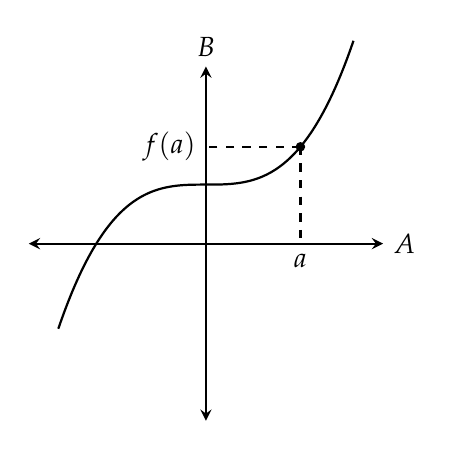
\begin{tikzpicture}[scale=1.5]
	\draw[<->,thick] (-1.5,0) -- (1.5,0) node[right] {$A$};
	\draw[<->,thick] (0,-1.5) -- (0,1.5) node[above] {$B$};
	\draw[thick, domain=-1.25:1.25, samples=200, variable=\x] plot (\x, {(5*\x^3 + 4)/8});
	\filldraw (0.8,0.82) circle (1pt);
	\draw[thick,dashed] (0.8,0.82) -- (0,0.82) node[left] {$f(a)$};
	\draw[thick,dashed] (0.8,0.82) -- (0.8,0) node[below] {$a$};
\end{tikzpicture}\]
This is a relation from $A$ to $B$. In this way, a function is a special case of a relation.

\item[(2)] Let 
\[S = \setp{(x,y) \in \rr^2}{x^2 + y^2 = 1} \subseteq \rr \times \rr,\]
this is a relation from $\rr$ to $\rr$.
\[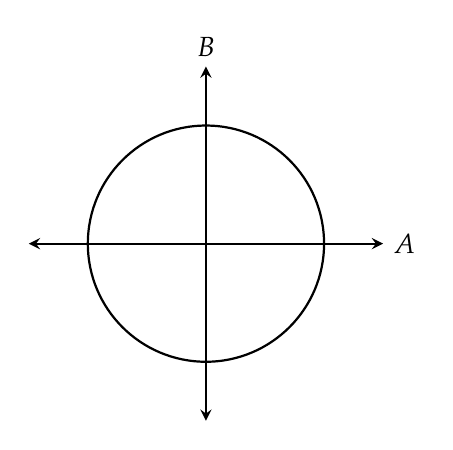
\begin{tikzpicture}[scale=1.5]
	\draw[<->,thick] (-1.5,0) -- (1.5,0) node[right] {$A$};
	\draw[<->,thick] (0,-1.5) -- (0,1.5) node[above] {$B$};
	\draw[thick] (0,0) circle (1);
\end{tikzpicture}\]
Solving for $y$ gives \[y = \pm \sqrt{1 - x^2}\]
This is a \emph{multi-valued function} (fails the vertical line test) defined on $[-1,1]$. We usually do not call such things functions, but it is a legitimate relation on $\rr$.
\end{itemize}
\end{example}

\vspace*{1em}

\begin{definition}
Let $R \subseteq A \times B$ be a relation from $A$ to $B$. The \cdef{domain\ of} {\color{blue}$R$} is
\[\dom(R) = \setp{a \in A}{(a,b) \in R \text{ for some $b \in B$}}\]
This is the set of all first coordinates that occur in elements of $R$.\\
\\
The \cdef{range\ of} {\color{blue}$R$} (also called \cdef{image\ of} {\color{blue}$R$}) is
\[\range(R) = \setp{b \in B}{(a,b) \in R \text{ for some $a \in A$}}\]
This is the set of all second coordinates that occur in elements of $R$.\\
\\
Visually, for example,
\[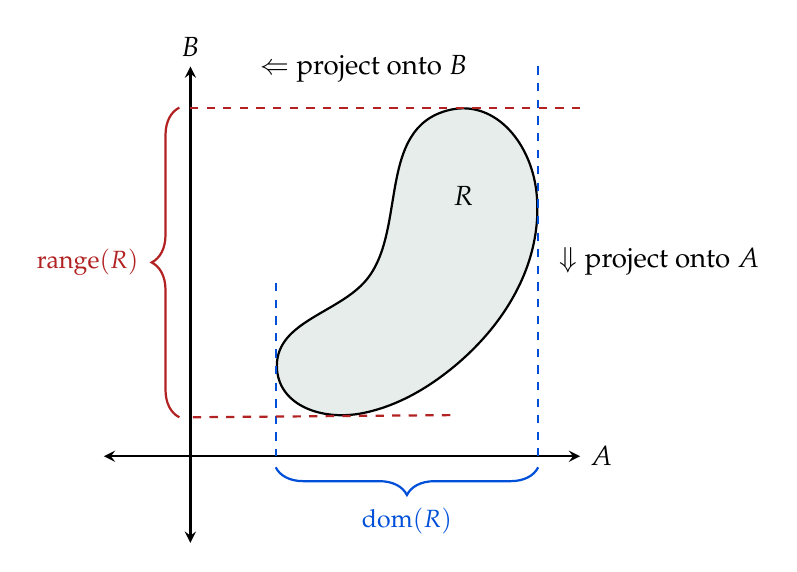
\begin{tikzpicture}[scale=1.1]
    \draw[<->,thick] (-1,0)--(4.5,0) node[right] {$A$};
	\draw[<->,thick] (0,-1)--(0,4.5) node[above] {$B$};
    \node[] at (3.15,3) {$R$};
    
    \path[draw,thick,use Hobby shortcut,closed=true,fill=forest,fill opacity=1/10]
(1,1) .. (2,0.5) .. (3,1) .. (4,3) .. (3,4) .. (2,2) .. (1,1);

	\draw[thick,dashed,newblue] (0.985,2) -- (0.985,0);
	\draw[thick,dashed,newblue] (4.015,4.5) -- (4.015,0);
	\draw[thick,dashed,firebrick] (4.5,4.025) -- (0,4.025);
	\draw[thick,dashed,firebrick] (3,0.475) -- (0,0.45);
	
	\draw [decorate,decoration={brace,amplitude=10pt,mirror,raise=4pt},yshift=0pt,thick,newblue]
(0.985,0) -- (4.015,0) node [black,midway,below,yshift=-1.5em] {\small$\color{newblue}\dom(R)$};
	\draw [decorate,decoration={brace,amplitude=10pt,mirror,raise=4pt},yshift=0pt,thick,firebrick]
(0,4.025) -- (0,0.45) node [black,midway,left,xshift=-1.5em] {\small$\color{firebrick}\range(R)$};

    \node[right] at (4.15,2.25) {$\Downarrow$ project onto $A$};
    \node[above] at (2,4.2) {$\Leftarrow$ project onto $B$};

\end{tikzpicture}\]
\end{definition}

%\vspace*{1em}

\begin{definition}
Let $R \subseteq A \times B$ be a relation from $A$ to $B$. The \cdef{inverse\ relation} {\color{blue}$R^{-1}$} is
\[R^{-1} = \setp{(b,a) \in B \times A}{(a,b) \in R},\]
a relation from $B$ to $A$.
Visually, for example,
\[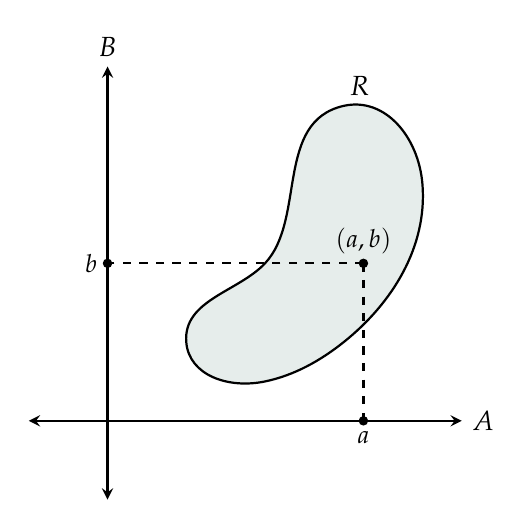
\begin{tikzpicture}
    \draw[<->,thick] (-1,0)--(4.5,0) node[right] {$A$};
	\draw[<->,thick] (0,-1)--(0,4.5) node[above] {$B$};
    \node[above] at (3.2,4) {$R$};
    
    \path[draw,thick,use Hobby shortcut,closed=true,fill=forest,fill opacity=1/10]
(1,1) .. (2,0.5) .. (3,1) .. (4,3) .. (3,4) .. (2,2) .. (1,1);

	\filldraw (3.25,2) circle (1.5pt) node[above] {\small$(a,b)$};
	\draw[thick,dashed] (3.25,2) -- (3.25,0) node[below] {\small $a$};
	\draw[thick,dashed] (3.25,2) -- (0,2) node[left] {\small $b$};
	\filldraw (3.25,0) circle (1.5pt);
	\filldraw (0,2) circle (1.5pt);
\end{tikzpicture}
\qquad
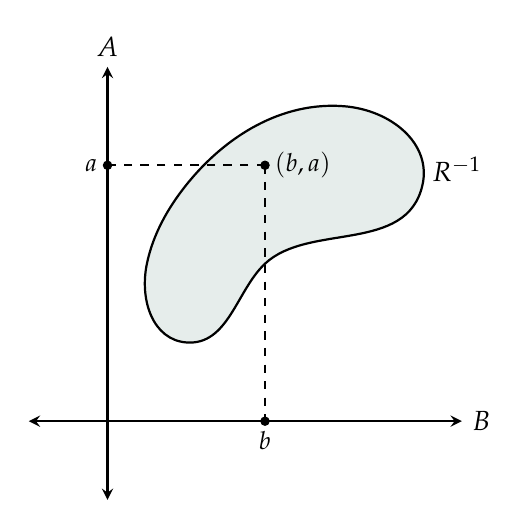
\begin{tikzpicture}
    \draw[<->,thick] (-1,0)--(4.5,0) node[right] {$B$};
	\draw[<->,thick] (0,-1)--(0,4.5) node[above] {$A$};
    \node[right] at (4,3.2) {$R^{-1}$};
    
    \path[draw,thick,use Hobby shortcut,closed=true,fill=forest,fill opacity=1/10]
(1,1) .. (0.5,2) .. (1,3) .. (3,4) .. (4,3) .. (2,2) .. (1,1);

	\filldraw (2,3.25) circle (1.5pt) node[right] {\small$(b,a)$};
	\draw[thick,dashed] (2,3.25) -- (0,3.25) node[left] {\small $a$};
	\draw[thick,dashed] (2,3.25) -- (2,0) node[below] {\small $b$};
	\filldraw (0,3.25) circle (1.5pt);
	\filldraw (2,0) circle (1.5pt);
\end{tikzpicture}
\]
If $A = B$, then we obtain $R^{-1}$ by reflecting along the \emph{diagonal}, this is the subset defined as \[\Delta_A = \setp{(a,a)}{a \in A} \subseteq A \times A.\]
\[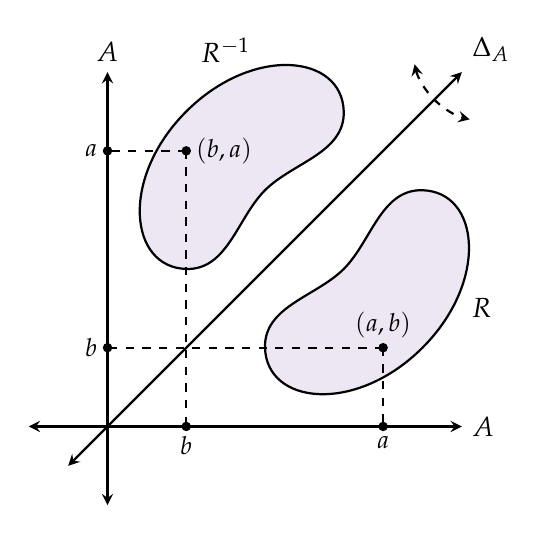
\begin{tikzpicture}
    \draw[<->,thick] (-1,0)--(4.5,0) node[right] {$A$};
	\draw[<->,thick] (0,-1)--(0,4.5) node[above] {$A$};
	\draw[<->,thick] (-0.5,-0.5)--(4.5,4.5) node[above right] {$\Delta_A$};
    \node[right] at (4.5,1.5) {$R$};
    \node[above] at (1.5,4.5) {$R^{-1}$};
    
    \path[draw,thick,use Hobby shortcut,closed=true,fill=indigo,fill opacity=1/10]
(2,1) .. (4,1) .. (4,3) .. (3,2) .. (2,1);

	\filldraw (3.5,1) circle (1.5pt) node[above] {\small$(a,b)$};
	\draw[thick,dashed] (3.5,1) -- (3.5,0) node[below] {\small $a$};
	\draw[thick,dashed] (3.5,1) -- (0,1) node[left] {\small $b$};
	\filldraw (3.5,0) circle (1.5pt);
	\filldraw (0,1) circle (1.5pt);

    \path[draw,thick,use Hobby shortcut,closed=true,fill=indigo,fill opacity=1/10]
(1,2) .. (1,4) .. (3,4) .. (2,3) .. (1,2);

	\filldraw (1,3.5) circle (1.5pt) node[right] {\small$(b,a)$};
	\draw[thick,dashed] (1,3.5) -- (0,3.5) node[left] {\small $a$};
	\draw[thick,dashed] (1,3.5) -- (1,0) node[below] {\small $b$};
	\filldraw (0,3.5) circle (1.5pt);
	\filldraw (1,0) circle (1.5pt);

    \path[draw,thick,use Hobby shortcut,dashed,<->]
(3.9,4.6) .. (4.15,4.15) .. (4.6,3.9);
\end{tikzpicture}\]
\end{definition}

\vspace*{1em}

\begin{example}
In the special case of a bijection $f:A \to B$, its graph is a relation
\[\Gamma(f) = \setp{(a,b) \in A \times B}{b = f(a)} \leftrightarrow f\]
Its inverse relation is
\begin{align*}
\Gamma(f)^{-1} &= \setp{(b,a) \in B \times A}{(a,b) \in \Gamma(f)}\\[0.5em]
 &= \setp{(b,a) \in B \times A}{b = f(a)}\\[0.5em]
 &= \setp{(b,a) \in B \times A}{a = f^{-1}(b)}\\[0.5em]
 &= \Gamma(f^{-1})
\end{align*}
\end{example}

%\vspace*{1em}

\begin{example}
Consider sets $A = \set{1,2,3,4,5}$ and $B = \set{u,v,w,x,y,z}$. Then consider the following relation from $A$ to $B$.
\[R = \set{(1,z),(2,v),(4,x),(2,v),(4,u),(5,w),(2,x)}\]
The domain of $R$ is the list of those elements of $A$ that appear as first coordinates of elements of $R$, that is,
\[\dom(R) = \set{1,2,4,5}.\]
While the range of $R$ is the list of those elements of $B$ that appear as second coordinates of elements of $R$, that is,
\[\range(R) = \set{u,v,w,x,z}.\]
The inverse relation from $B$ to $A$ is obtained by swapping the first and second coordinates
\[R^{-1} = \set{(z,1),(v,2),(x,4),(v,2),(u,4),(w,5),(x,2)} \subseteq B \times A\]
\end{example}

\vspace*{2em}

\begin{mdframed}
\begin{center}
{\Large Properties of Relations}
\end{center}
\end{mdframed}
From now on we assume $B = A$; a relation from $A$ to $A$ is called a \emph{relation on $A$}. 

\vspace*{1em}

\begin{example}[Equality]
Consider the following relation on $A$, the diagonal
\[R = \Delta_A = \setp{(a,a)}{a \in A}\]
For this relation, we have
\[aRb \quad \text{if and only if} \quad (a,b) \in R \quad \text{if and only if} \quad a = b\]
So, this $R$ corresponds to the usual equality relation. We generalise the concept of equality to ``equivalence''. For this, we first record the most fundamental properties of equality.
\begin{itemize}
\item[(i)] $a = a$ for every $a \in A$.
\item[(ii)] If $a = b$, then $b = a$, for every $a,b \in A$.
\item[(iii)] If $a = b$ and $b = c$, then $a = c$, for every $a,b,c \in A$.
\end{itemize}
\end{example} 

\vspace*{1em}

\begin{definition}
Let $R$ be a relation on $A$, that is, $R \subseteq A \times A$.
\begin{itemize}[itemsep=1em]
\item $R$ is said to be \cdef{reflexive} if $xRx$ for every $x \in A$, that is, if $(x,x) \in R$ for every $x \in A$.\\
\\
Set theoretically, this is saying that we require $\Delta_A \subseteq R$.

\item $R$ is said to be \cdef{symmetric} if $xRy$ implies $yRx$ for every $x,y \in A$, that is, if $(x,y) \in R$ implies $(y,x) \in R$ for every $x,y \in A$.\\
\\
Set theoretically, this is saying that we require $R = R^{-1}$.

\item $R$ is said to be \cdef{transitive} if $xRy$ and $yRz$ implies $xRz$ for every $x,y,z \in A$, that is, if $(x,y),(y,z) \in R$ implies $(x,z) \in R$ for every $x,y,z \in A$.
\end{itemize}
\end{definition}

\vspace*{1em}

\begin{example}
Consider the set $A = \set{a,b,c}$, and the following relation on $A$
\[R = \set{(a,a),(b,b),(c,c),(a,b),(b,c),(a,c)}\]
Note that
\begin{itemize}[leftmargin=*]
\item[] $R$ is reflexive, since $(a,a),(b,b),(c,c) \in R$.
\item[] $R$ is \emph{not} symmetric, since $(a,b) \in R$ but $(b,a) \notin R$.
\item[] $R$ is transitive, $(a,b),(b,c),(a,c) \in R$ etc.
\end{itemize}
\end{example}

\vspace*{1em}

\begin{example}
Let $A = \rr$, and consider the following relation $R$ on $\rr$
\[R = \setp{(x,y) \in \rr^2}{\abs{x-y} \leq 1}\]
For any $(x,y) \in R$ we have $\abs{x - y} \leq 1$ and therefore $-1 \leq x - y \leq 1$. Hence $R$ is bounded by the lines given as $x - y = -1$ and $x - y = 1$, or equivalently, the lines $y = x + 1$ and $y = x-1$
\[\text{\color{red}insert image}\]
Is $R$  reflexive, symmetric  or transitive?\\
\\
Note that $R$ contains the diagonal line, hence $R$ is reflexive. This is the fact that 
\[\abs{x - x} = 0 \leq 1,\ \text{ so } (x,x) \in R\]\\
Furthermore, $R$ is symmetric along the diagonal. This is the fact that
\[\abs{y - x} = \abs{x - y} \leq 1,\ \text{ so if $(x,y) \in R$, then $(y,x) \in R$}\]\\
Is $R$ transitive? This is then asking that if $\abs{x - y} \leq 1$ and $\abs{y - z} \leq 1$, then is $\abs{x - z} \leq 1$.\\[0.5em]
%For any point $U \in R$, go horizontally to reach a diagonal point $Z \in R$. Mover vertically from $Z$, within $R$, and choose any point $V$. Completing a rectangle with these three vertices $U,Z,V$, is the fourth vertex $W$ in $R$? Not necessarily, thus $R$ is no transitive.\\
%\\
We exhibit a counterexample to conclude that $R$ is not transitive. Consider $x = 1.5,\ y = 1$ and $z = 0$. Then since
\[\abs{x - y} = \abs{1.5 - 1} = 0.5 \leq 1 \quad \text{and} \quad \abs{y - z} = \abs{1 - 0} = 1 \leq 1,\]
therefore $(x,y),(y,z) \in R$. But \[\abs{x - z} = \abs{1.5 - 0} = 1.5 > 1\] and thus $(x,z) \notin R$. Therefore $R$ is not transitive.
\end{example}
\newpage

\section{Equivalence Relations}
\vspace*{1em}

\begin{definition}
Let $R$ be a relation on $A$. We call $R$ an \cdef{equivalence\ relation} if
\begin{multicols}{3}
\begin{itemize}
\item[$\bullet$] $R$ is reflexive
\item[$\bullet$] $R$ is symmetric
\item[$\bullet$] $R$ is transitive
\end{itemize}
\end{multicols}
In this case, if $aRb$, then we say $a$ is equivalent to $b$ and we alternatively denote it as $a \sim b$ (by symmetry, $b \sim a$ as well).
\end{definition}

\vspace*{1em}

An equivalence relation is a generalisation of equality.
\begin{example}
$R = \Delta_A = \setp{(a,a)}{a \in A}$ is an equivalence relation.
\[aRb\ \text{ if and only if }\ a = b \quad \text{and} \quad R = ``=''\]
Since,
\begin{itemize}
\item[(i)] $a = a$ for every $a \in A$.
\item[(ii)] If $a = b$, then $b = a$, for every $a,b \in A$.
\item[(iii)] If $a = b$ and $b = c$, then $a = c$, for every $a,b,c \in A$.
\end{itemize}
\end{example}

\vspace*{1em}

\begin{example}\label{example:eqrel1}
For $A = \set{1,2,3,4,5}$, consider the following relation on $A$
\[R = \set{(1,1),(2,2),(3,3),(4,4),(5,5),(1,3),(1,5),(5,1),(5,3),(3,1),(3,5),(2,4),(4,2)} \subseteq A \times A\]
$R$ is an equivalence relation. Note,
\begin{itemize}
\item[(i)] for every $a \in A$, we have $(a,a) \in A$.
\item[(ii)] Whenever $(a,b) \in R$, we have $(b,a) \in R$. (e.g. $(1,3) \in R$ and $(3,1) \in R$, $(3,6),(6,3) \in R$ etc.)
\item[(iii)] We have $(1,6),(6,3) \in R$, is $(1,3) \in R$? Yes! Check remaining cases.
\end{itemize}
\end{example}

\vspace*{1em}

\begin{example}\label{example:eqrel2}
Consider the following relation on $\rr^2\setminus\set{(0,0)}$
\[(x,y)R(a,b) \quad \text{if and only if (i.e. the definition)} \quad \text{there exists $\lambda \in \rr_{\neq 0}$ such that $(a,b) = (\lambda x,\lambda y)$}\]
We show $R$ is an equivalence relation.
\begin{itemize}
\item[(i)] Note that for $\lambda = 1$, we have
\[(x,y) = (\lambda x,\lambda y)\]
Therefore $(x,y)R(x,y)$, for all $(x,y) \in \rr^2$, and hence $R$ is reflexive.

\item[(ii)] Suppose $(x,y),(a,b) \in \rr^2$ is such that $(x,y)R(a,b)$. Therefore $(a,b) = (\lambda x,\lambda y)$, for some $\lambda \in \rr_{\neq 0}$, and hence $a = \lambda x,\,b = \lambda y$. Thus,
\[(x,y) = ((1/\lambda)a,(1/\lambda)b).\]
Therefore $(a,b)R(x,y)$, and hence $R$ is symmetric.

\item[(iii)] Suppose $(x,y),(a,b),(u,v) \in \rr^2$ is such that $(x,y)R(a,b)$ and $(a,b)R(u,v)$. Therefore $(a,b) = (\lambda x,\lambda y)$ and $(u,v) = (\mu a,\mu b)$, for some $\lambda,\mu \in \rr_{\neq 0}$. Hence \[a = \lambda x,\,b = \lambda y\; \text{ and }\; u = \mu a,\, v = \mu b.\] Thus,
\[(u,v) = (\mu\lambda x,\mu\lambda y).\]
Therefore $(x,y)R(u,v)$, and hence $R$ is transitive.
\end{itemize}
\end{example}

\vspace*{1em}

\begin{example}\label{example:eqrel3}
For $A = \set{\text{all people}}$, consider the following relation on $A$
\[P_1 \sim P_2 \quad \text{if and only if} \quad \text{age}(P_1) = \text{age}(P_2)\]
This is an equivalence relation. Try and verify the definition!
\end{example}

\vspace*{1em}

\begin{definition}
Let $R$ be an equivalence relation on $A$.\\[0.5em]
For $a \in A$, define the {\color{blue}$R$-}\cdef{equivalence\ class\ represented\ by} {\color{blue}$a$} to be the subset
\begin{align*}
[a] &= \setp{x \in A}{xRa \text{ (or $aRx$, by symmetry)}} = \set{\text{all elements of $A$ that are equivalent to $a$}} \subseteq A\\[0.5em]
 &= \setp{x \in A}{\text{$(x,a) \in R$ ($(a,x) \in R$)}}
\end{align*}
Since $R$ is reflexive, that is, $aRa$, we have $a \in [a]$ for any $a \in A$.
\end{definition}

\vspace*{1em}

\begin{example}
Let us find the equivalence classes for \[R = \set{(1,1),(2,2),(3,3),(4,4),(5,5),(1,3),(1,5),(5,1),(5,3),(3,1),(3,5),(2,4),(4,2)}\] described in Example \ref{example:eqrel1} on $A = \set{1,2,3,4,5}$.
\begin{align*}
[1] &= \text{the equivalence class of $1$}\\[0.5em]
 &= \text{all elements ``equivalent'' (that is, $R$-related) to $1$}\\[0.5em]
 &= \setp{x \in A}{(x,1) \in R}\\[0.5em]
 &= \set{1,3,5},\quad \text{since $(1,1),(3,1) \in R$}
\end{align*}
Similarly, 
\begin{align*}
[2] &= \setp{x \in A}{(x,2) \in R} & [4] &= \setp{x \in A}{(x,4) \in R}\\[0.5em]
 &= \set{2,4} & &= \set{2,4} = [2]\\[1em]
%
[3] &= \setp{x \in A}{(x,3) \in R} & [5] &= \setp{x \in A}{(x,5) \in R}\\[0.5em]
 &= \set{1,3,5} & &= \set{1,3,5} = [1] = [3]
\end{align*}
So, 
\begin{align*}
[1] &= [3] = [5] = \set{1,3,5}\\[0.5em]
[2] &= [4] = \set{2,4}\\
\end{align*}
We make the following observations: for $a,b \in A$,
\begin{align*}
\text{if $a\cancel{R}b$},& \text{ then $[a] \cap [b] = \emptyset$; and}\\[0.5em]
\text{if $aRb$},& \text{ then $[a] = [b]$}
\end{align*}
\end{example}

\vspace*{1em}

\begin{example}
Consider the equivalence relation as described in Example \ref{example:eqrel2}. Let's compute the equivalence class of $(3,5) \in \rr^2$
\begin{align*}
[(3,5)] &= \setp{(x,y) \in \rr^2}{(3,5) R (x,y)}\\[0.5em]
 &= \setp{(x,y) \in \rr^2}{(x,y) = (3\lambda,5\lambda),\ \text{ for some $\lambda \in \rr_{\neq 0}$}}\\[0.5em]
 &= \setp{(x,y) \in \rr^2}{x = 3\lambda\ \text{ and }\ y = 5\lambda,\ \text{ for some $\lambda \in \rr_{\neq 0}$}}\\[0.5em]
 &= \setp{(3\lambda,5\lambda) \in \rr^2}{\lambda \in \rr_{\neq 0}}
\end{align*}
This is nothing but the line defined by the equation $3y = 5x$, minus the origin.
\end{example}

\vspace*{1em}

\begin{example}
Consider the equivalence relation as described in Example \ref{example:eqrel3}. Let's compute the equivalence class of me!
\begin{align*}
[\text{Deewang}] &= \setp{P \in A}{P \sim \text{Deewang}}\\[0.5em]
 &= \setp{P \in A}{\text{age}(P) = \text{age}(\text{Deewang}) = 28}\\[0.5em]
 &= \set{\text{all people that are $28$ years of age}}
\end{align*}
\end{example}

\vspace*{1em}

\begin{example}[Congruence is an Equivalence Relation]\label{example:congeq}
Let $A = \zz$ and fix a positive integer $n$. Define a relation $R$ on $\zz$ as
\[aRb \text{ if and only if } a\equiv b \modar{n}\]
Recall that we say $a\equiv b\modar{n}$ if $n\mid (a - b)$. This is an equivalence relation.
\begin{itemize}[itemsep=1em]
\item[(i)] $a \equiv a \modar{n}$, for every $a \in \zz$.\\[0.5em]
This is because $n\mid (a-a)$ for every integer $a$, as $a - a = 0 = n\cdot 0$.

\item[(ii)] If $a \equiv b \modar{n}$, then $b \equiv a \modar{n}$, for every $a,b \in \zz$.\\[0.5em]
This is because if $a \equiv b \modar{n}$, then $n\mid (a - b)$. That is, $a - b = nk$ for an integer $k$. Therefore $b - a = n(-k)$; since $-k \in \zz$, hence $n\mid (b-a)$. Thus $b \equiv a \modar{n}$.

\item[(iii)] If $a \equiv b \modar{n}$ and $b \equiv c \modar{n}$, then $a \equiv c \modar{n}$, for every $a,b,c \in \zz$.\\[0.5em]
This is because if $a \equiv b \modar{n}$ and $b \equiv c \modar{n}$, then $n\mid (a - b)$ and $n \mid (b-c)$. That is, $a - b = nk$ and $b - c = n\ell$ for integers $k,\ell$. Therefore $a - c = (a - b) + (b - c) = n(k + \ell)$; since $k + \ell \in \zz$, hence $n\mid (a-c)$. Thus $a \equiv c \modar{n}$.
\end{itemize}
Thus the congruence relation ``$\equiv$'' is an equivalence relation.\\
\\
Let $n = 5$, we find the equivalence class of $3$ with respect to the congruence modulo $5$ relation.
\begin{align*}
[3]_5 &= \setp{n \in \zz}{n \equiv 3 \modar{5}}\\[0.5em]
 &= \setp{n \in \zz}{5\mid (n - 3)}\\[0.5em]
 &= \setp{n \in \zz}{n - 3 = 5k\text{, for some integer $k$}}\\[0.5em]
 &= \setp{n \in \zz}{n = 5k + 3\text{, for some integer $k$}}\\[0.5em]
 &= \setp{5k + 3}{k \in \zz}\\[0.5em]
 &= \set{\ldots,-7,-2,3,8,13,\ldots}\\[0.5em]
 &= \set{\text{all integers that leave remainder $3$ when divided by $5$}}
\end{align*}
\end{example}

\vspace*{1em}

\begin{example}
Let $A = \zz$, we define a relation $R$ on $\zz$ as
\[aRb \text{ if and only if } a + 3b \text{ is even}\]
We show this is an equivalence relation.
\begin{itemize}
\item[(i)] Is $aRa$, for every $a \in \zz$?\\[0.5em]
Since for any $a \in \zz$, we have that $a + 3a = 4a$ is even. Thus $aRa$, and so $R$ is reflexive.

\item[(ii)] Does $aRb$ imply $bRa$?\\[0.5em]
Suppose $aRb$, that is, $a + 3b$ is even. We show $bRa$, or $b + 3a$ is even. Note that $(a + 3b) + (b + 3a) = 4a + 4b$ is even, therefore $b + 3a = 4(a+b) - (a + 3b)$ is even, as a sum of even integers. Hence $bRa$, and thus $R$ is symmetric.

\item[(iii)] Do $aRb$ and $bRc$ imply $aRc$?\\[0.5em]
Suppose $aRb$ and $bRc$, that is, $a + 3b$ and $b + 3c$ is even. We show $aRc$, or $a + 3c$ is even. Note that $(a + 3b) + (b + 3c) = a + 3c + 4b$, therefore $a + 3c = (a + 3b) + (b + 3c) - 4b$ is even, as a sum of even integers. Hence $aRc$, and thus $R$ is transitive.
\end{itemize}
Thus, $R$ is an equivalence relation.

%\vspace*{1em}
%
%\begin{remark}
%Note that
%\begin{align*}
%aRb &\text{ if and only if } a + 3b \equiv 0 \modar{2}\\[0.5em]
% &\text{ if and only if } a \equiv -3b \modar{2}\\[0.5em]
% &\text{ if and only if } a \equiv b \modar{2} \quad \text{since $-3b \equiv b\modar{2}$, as $2\mid (-3b-b)$}
%\end{align*}
%Thus $R$ was simply the congruence relation modulo $2$ and hence is an equivalence relation. Thus,
%\begin{align*}
%[0] &= \setp{x \in \zz}{xR0}\\[0.5em]
% &= \setp{x \in \zz}{x \equiv 0 \modar{2}}\\[0.5em]
% &= \set{\text{all even integers}}\\[1em]
%%
%[1] &= \setp{x \in \zz}{xR1}\\[0.5em]
% &= \setp{x \in \zz}{x \equiv 1 \modar{2}}\\[0.5em]
% &= \set{\text{all odd integers}}
%\end{align*}
%Thus, under $R$, there are two distinct equivalence classes
%\[E = \set{\text{all even integers}},\ O = \set{\text{all odd integers}}\]
%Note: $E \cap O = \emptyset$ and $E \cup O = \zz$
%\end{remark}
\end{example}

\vspace*{2em}

\begin{mdframed}
\begin{center}
{\Large Properties of Equivalence Classes}
\end{center}
\end{mdframed}

\begin{theorem}\label{thm:eq=eqcl}
Let $R$ be an equivalence relation on a set $A$. Then, for $a, b \in A$,
\[ [a] = [b] \text{ if and only if } aRb\]
\end{theorem}
\begin{proof}
Let $a,b \in A$.
\begin{itemize}
\item[$(\Rightarrow)$] Suppose $[a] = [b]$, we show $aRb$. Note that, since $R$ is reflexive, we have $aRa$. Therefore, $a \in [a] = [b]$, and hence $a \in [b]$. Thus, $aRb$.

\item[$(\Leftarrow)$] Suppose $aRb$, we show $[a] = [b]$, that is, we show $[a] \subseteq [b]$ and $[b] \subseteq [a]$. Note that since $R$ is symmetric, we also have $bRa$.\\[0.5em]
Consider any $x \in [a]$, by definition, $xRa$. Since $xRa$ and $aRb$, by assumption, we obtain $xRb$, by transitivity. Therefore, $x \in [b]$, and hence $[a] \subseteq [b]$.\\[0.5em]
Consider any $y \in [b]$, by definition, $yRb$. Since $yRb$ and $bRa$, by assumption, we obtain $yRa$, by transitivity. Therefore, $y \in [a]$, and hence $[b] \subseteq [a]$.\\[0.5em]
Thus, $[a] = [b]$.
\end{itemize}
\end{proof}

\vspace*{1em}

We have shown that $a$ and $b$ are equivalent, if and only if $[a] = [b]$. As a consequence, we obtain the following.
\begin{theorem}
Let $R$ be an equivalence relation on a set $A$. Then, for $a, b \in A$, if $[a] \cap [b] \neq \emptyset$, then $[a] = [b]$.
\end{theorem}
Thus, given any two equivalence classes $[a]$ and $[b]$, they are either disjoint or identical.
\begin{proof}
Let $a,b \in A$, and suppose $[a] \cap [b] = \emptyset$. We show $[a] = [b]$. Consider any $x \in [a] \cap [b]$. Then $x \in [a]$ and $x \in [b]$, and therefore $xRa$ and $xRb$. Since $R$ is symmetric and $xRa$, we obtain $aRx$. Hence we have $aRx$ and $xRb$, and thus $aRb$ by transitivity of $R$. Therefore $[a] = [b]$, by Theorem \ref{thm:eq=eqcl}.
\end{proof}

\vspace*{1em}

\begin{remark}
Recall that a \cdef{partition} of $A$ is a collection of subsets $X_\alpha \subseteq A$, where $\alpha \in I$ for some index set (that is, for each element $\alpha \in I$, we have a subset $X_\alpha$) such that
\begin{align*}
X_\alpha \cap X_\beta = \emptyset &\text{ if } \alpha \neq \beta\\[0.5em]
\bigcup_{\alpha \in I}X_\alpha = A
\end{align*}
In this case, write $\displaystyle A = \coprod_{\alpha \in I}X_\alpha$ (``disjoint union'').
\end{remark}

\vspace*{1em}

\begin{theorem}
Let $R$ be an equivalence relation on a set $A$. Then, the collection of all $R$-equivalence classes defines a partition of $A$.\\[0.5em]
\emph{This partition is denoted $A/R$ (read as: ``$A$ mod $R$''), and is called \emph{the quotient set of $A$ by $R$.}}
\end{theorem}
\begin{proof}
The proof follows from the theorems above. We leave it to the reader to work out the details and write out a formal proof.
\end{proof}

\vspace*{1em}

Conversely,
\begin{theorem}
Let $\mathscr{S} = \set{X_\alpha}_{\alpha \in I}$ be a partition of a set $A$. Then, there exists a unique relation $R$ on $A$ such that the resulting partition by equivalence classes is the partition given
\end{theorem}
This is saying that \emph{giving an equivalence relation on $A$ is equivalent to defining a partition of $A$}.
\begin{proof}[Sketch of Proof]\renewcommand{\qed}{}
We first prove the existence of such a relation $R$ on $A$. Define $R$ as follows: say,
\[aRb \text{ if and only if } a,b \in X_\alpha \text{ for some $\alpha$}\]
for any $a,b \in A$. One checks that this $R$ is equivalent, verifying that $R$ is reflexive and symmetric is straightforward. Following is the argument for showing transitivity of $R$.\\[0.5em]
Suppose $aRb$ and $bRc$. By definition $a,b \in X_\alpha$ and $b,c \in X_\beta$. Therefore $b \in X_\alpha$ and $b \in X_\beta$, that is, $b \in X_\alpha \cap X_\beta$. Unless $X_\alpha = X_\beta$, we have shown that $X_\alpha \cap X_\beta \neq \emptyset$ contradicting the fact $\mathscr{S}$ is a partition. Hence, $X_\alpha = X_\beta$ and thus $a,c \in X_\alpha$. Therefore $aRc$.\\
\\
We still need to check following: (1) that $X_\alpha$ is an equivalence class for any $\alpha \in I$, we do this by exhibiting that for any $a \in X_\alpha$ we have $X_\alpha = [a]$; (2) This $R$ is the unique relation with this property.
\end{proof}

%\vspace*{1em}
%
%\begin{remark}
%We note that
%\[(a,b) \in R \text{ if and only if } aRb \text{ if and only if } a,b \in X_\alpha \text{ if and only if } (a,b) \in X_\alpha \times X_\alpha\]
%for some $\alpha \in I$. Therefore, as a subset $R \subseteq A \times A$, we have
%\[R = \coprod_{\alpha\in I} (X_\alpha \times X_\alpha)\]
%\end{remark}
%
\vspace*{1em}

\begin{example}
Let $A = \set{1,2,3,4,5,6}$, and consider a partition
\[\mathscr{S} = \set{\set{1,2},\set{3,4},\set{5,6}}\]
What is the equivalence relation $R$ reproducing this partition?\\
\\
Let $X_\alpha = \set{1,2},X_\beta = \set{3,4}$ and $X_\gamma = \set{5,6}$.
\begin{align*}
\text{Since $1,2 \in \set{1,2}$, we have}& \text{ $1R2$ or $(1,2) \in R \subseteq A \times A$}\\[0.5em]
\text{Since $3,4 \in \set{3,4}$, we have}& \text{ $3R4$ or $(3,4) \in R \subseteq A \times A$}\\[0.5em]
\text{Since $5,6 \in \set{5,6}$, we have}& \text{ $5R6$ or $(5,6) \in R \subseteq A \times A$}
\end{align*}
%What is the totality of $R$ as a subset of $A \times A$?
%\begin{align*}
%R &= (X_\alpha \times X_\alpha) \cup (X_\beta \times X_\beta) \cup (X_\gamma \times X_\gamma)\\[0.5em]
% &= \set{(1,2),(2,1),(1,1),(2,2)} \cup \set{(3,4),(4,3),(3,3),(4,4)} \cup \set{(5,6),(6,5),(5,5),(6,6)}\\[0.5em]
% &= \set{(1,1),(2,2),(3,3),(4,4),(1,2),(2,1),(3,4),(4,3),(5,6),(6,5)}
%\end{align*}
\end{example}

\vspace*{2em}

\begin{mdframed}
\begin{center}
{\Large Congruence modulo $n$}
\end{center}
\end{mdframed}

\begin{discussion}
Fix a positive integer $n \geq 2$. Recall that we say $a \equiv b \modar{n}$ if 
\[n\mid (a-b) \text{ if and only if $a$ and $b$ have the same remainder when divided by $n$}\]
We have seen in Example \ref{example:congeq} that \emph{congruence modulo $n$} is an equivalence relation. What are the equivalence classes?
\begin{align*}
[0] &= \setp{x \in \zz}{x \equiv 0 \modar{n}} = \setp{nk}{k \in \zz}\\[0.5em]
[1] &= \setp{x \in \zz}{x \equiv 1 \modar{n}} = \setp{nk + 1}{k \in \zz}\\[0.5em]
	&= \qquad \vdots\\[0.5em]
[n-1] &= \setp{x \in \zz}{x \equiv n-1 \modar{n}} = \setp{nk + (n-1)}{k \in \zz}
\end{align*}
Since $n \in [0]$, therefore $[n] = [0]$.\\[0.5em]
Similarly, since $n + 1 \in [1]$, therefore $[n+1] = [1]$; so on and so forth.\\
Note that the above list is of the form $[r]$ for $0 \leq r \leq n$, all possible remainders when a number is divided by $r$. In particular, for any integer $x \in \zz$, when divided by $n$, we have a quotient $q$ and remainder $r$ such that $x = nq + r$, and thus $x \in [r]$. Hence, $[0],[1],\ldots,[n-1]$ is the complete list of equivalence classes under the congruence relation modulo $n$.\\
\\
We denote the collection of distinct equivalence classes under congruence modulo $n$ as
\[\zz/n\zz = \underbrace{\set{[0],[1],\ldots,[n-1]}}_{\text{$n$-many elements}},\]
the set of \emph{integers modulo $n$}, read as ``$\zz$ mod $n\zz$''.\\
\\
Surprisingly, $\zz/n\zz$ has properties similar to that of $\zz$. We can define addition, subtraction and multiplication for elements in $\zz/n\zz$.
\begin{itemize}[leftmargin=*]
\item[]Addition. Given two elements $[a],[b] \in \zz/n\zz$, define
\[ [a] + [b] \defeq [a+b]\]
Here $[0]$ acts as a ``zero'' element under addition. That is,
\[ [a] + [0] = [a] = [0] + [a]\]

\item[]Multiplication. Given two elements $[a],[b] \in \zz/n\zz$, define
\[ [a] \cdot [b] \defeq [ab]\]
Here $[0]$ acts as a ``unit'' element under multiplication. That is,
\[ [a] \cdot [1] = [a] = [1] \cdot [a]\]
Also note that $[a] \cdot [0] = [0] = [0] \cdot [a]$.
\end{itemize}
\end{discussion}

%\vspace*{1em}

\begin{example}
For $n = 5$, consider $\zz/5\zz = \set{[0],[1],[2],[3],[4]}$.\\[1em]
\begin{minipage}{0.5\textwidth}
\begin{center}
{\renewcommand{\arraystretch}{1.5}%
\begin{tabular}{c|ccccc}
$+$ & $[0]$ & $[1]$ & $[2]$ & $[3]$ & $[4]$\\
\hline
$[0]$ & $[0]$ & $[1]$ & $[2]$ & $[3]$ & $[4]$\\
$[1]$ & $[1]$ & $[2]$ & $[3]$ & $[4]$ & $[0]$\\
$[2]$ & $[2]$ & $[3]$ & $[4]$ & $[0]$ & $[1]$\\
$[3]$ & $[3]$ & $[4]$ & $[0]$ & $[1]$ & $[2]$\\
$[4]$ & $[4]$ & $[0]$ & $[1]$ & $[2]$ & $[3]$\\
\end{tabular}
}
\end{center}
\[\text{addition table}\]
\end{minipage}\quad
\begin{minipage}{0.5\textwidth}
\begin{center}
{\renewcommand{\arraystretch}{1.5}%
\begin{tabular}{c|ccccc}
$\times$ & $[0]$ & $[1]$ & $[2]$ & $[3]$ & $[4]$\\
\hline
$[0]$ & $[0]$ & $[0]$ & $[0]$ & $[0]$ & $[0]$\\
$[1]$ & $[0]$ & $[1]$ & $[2]$ & $[3]$ & $[4]$\\
$[2]$ & $[0]$ & $[2]$ & $[4]$ & $[1]$ & $[3]$\\
$[3]$ & $[0]$ & $[3]$ & $[1]$ & $[4]$ & $[2]$\\
$[4]$ & $[0]$ & $[4]$ & $[3]$ & $[2]$ & $[1]$\\
\end{tabular}
}
\end{center}
\[\text{multiplication table}\]
\end{minipage}
\begin{proof}[Observation]\renewcommand{\qed}{}
In the multiplication table, we have
\[ [2]\cdot [3] = [1] = [3]\cdot [2] \quad \text{and} \quad [4]\cdot[4] = [1];\]
note that $[1]$ is ``unit'' element under multiplication.\newpage
In this way, we say
\begin{align*}
\text{$[2]$ is the ``inverse''}& \text{ of $[3]$}\\[0.5em]
\text{$[3]$ is the ``inverse''}& \text{ of $[2]$}\\[0.5em]
\text{$[4]$ is the ``inverse''}& \text{ of $[4]$}
\end{align*}
In this way, ``division'' in $\zz/5\zz$ is possible. ``Dividing'' by $[2]$ means multiplying by $[3]$, for example. 
\end{proof}
\end{example}

\vspace*{1em}

Division is not always possible for all $\zz/n\zz$.
\begin{example}
For $n = 4$, consider $\zz/4\zz = \set{[0],[1],[2],[3]}$.\\[1em]
\begin{center}
{\renewcommand{\arraystretch}{1.5}%
\begin{tabular}{c|cccc}
$\times$ & $[0]$ & $[1]$ & $[2]$ & $[3]$\\
\hline
$[0]$ & $[0]$ & $[0]$ & $[0]$ & $[0]$\\
$[1]$ & $[0]$ & $[1]$ & $[2]$ & $[3]$\\
$[2]$ & $[0]$ & $[2]$ & $[0]$ & $[2]$\\
$[3]$ & $[0]$ & $[3]$ & $[2]$ & $[1]$
\end{tabular}
}
\end{center}
\[\text{multiplication table}\]
For no $[a] \in \zz/4\zz$ do we get $[2]\cdot [a] = [1]$. So, ``dividing'' by $[2]$ has no meaning in $\zz/4\zz$. Thus, division is not possible in $\zz/4\zz$.
\end{example}

\vspace*{1em}

\begin{discussion}[Fact]
For a prime number $p,\ \zz/p\zz$ admits division.
\item[] If $n$ is not prime, you cannot do division in $\zz/n\zz$. If $n = ab,\ 1 < a,b < n$, then 
\[ [a] \cdot [b] = [n] = [0]\]
So, $[a],[b]$ are ``zero divisors''.\\
\\
In $\zz/p\zz$, where $p$ is a prime number, we can do all arithmetic operations: addition, subtraction, multiplication and division; this is an example of a \emph{field}.
\[\underbrace{\underbrace{\underbrace{\text{addition},\ \text{subtraction}}_{\text{group}},\ \text{multiplication}}_{\text{ring}},\ \text{division}}_{\text{field}}\]
\end{discussion}
\newpage

\section{Functions}
\vspace*{1em}

\begin{discussion}
Let $A,B$ be sets, recall that a function
\[f: A \to B\]
is a ``rule'' that assigns an element of $B$ to every element of $A$. We note the following.
\begin{itemize}
\item[(i)] $\dom(f) = A$. ($f$ is defined for every element of $A$)
\item[(ii)] For each $a \in A$, $f$ assigns a \emph{unique} element $f(a) \in B$.
\end{itemize}
We now give a formal definition of a function $f:A \to B$ in terms of relations.
\end{discussion}

\vspace*{1em}

\begin{definition}
Let $A,B$ be non-empty sets. A \cdef{function} {\color{blue}$f:A \to B$} is a relation $f \subseteq A \times B$ from $A$ to $B$ such that for every $a \in A$
\[\text{if $afb$ and $afc$, then $b = c$;}\]
or equivalently we have  \[\abs{f \cap (\set{a} \times B)} = 1\] i.e. for every $a \in A$, there is a single element in $f$ with $a$ as the first coordinate.\\
\\
That is, for every $a \in A$, there is a unique $b \in B$ that is $f$-related to $a$; that is, for every $a$, there is a unique $b$ such that $(a,b) \in f$. In this case, we write $b = f(a)$. Notationally, we have
\begin{align*}
f: A &\to B\\
 a&\mapsto b
\end{align*}
With the $a \mapsto b$ notation meaning $b = f(a)$.\\
\\
With this notation, a relation $f$ is a function if for any $a,c \in A$,
\[a = c \text{ implies } f(a) = f(c)\]
Verifying this property to show that a given relation is a function is called \emph{showing $f$ is well-defined}.\\
\\
As a relation, $f$ has a domain and range. We have $\dom(f) = A$ and $\range(f) = \setp{f(a)}{a \in A}$. To note, the range can be a proper subset of $B$; we call $B$ the \cdef{codomain} of $f$, we denote $\mathrm{codom}(f) = B$.

\vspace*{0.5em}

\begin{remark}
In terms of our notation, the function $f$ as a relation, that is, as a subset of $A \times B$, is
\[f = \setp{(a,f(a))}{a \in A} \subseteq A \times B,\]
which is what we usually call the \emph{graph of $f$}.
\end{remark}
\end{definition}

\vspace*{1em}

\begin{example}[some abstract examples]\hfill
\begin{itemize}
\item[$\bullet$] \emph{Identity function}.\\[0.5em]
For any set $X$, the \emph{identity function on $X$} is the function
\begin{align*}
\id_X: X &\to X\\
 x&\mapsto x
\end{align*}
That is, this is the function $\id_X(x) = x$. As a relation, this is just the diagonal subset
\[\id_X = \setp{(x,x)}{x \in X} \subseteq X \times X\]

\item[$\bullet$] \emph{Inclusion function}.\\[0.5em]
For any non-empty set $A$, and a subset $C \subseteq A$. The inclusion function is the function
\begin{align*}
\iota : C &\to A\\
 c&\mapsto c
\end{align*}
As a relation, this is the subset
\[\iota = \setp{(c,c)}{c \in C} \subseteq C \times A\]

\item[$\bullet$] \emph{Restriction function}.\\[0.5em]
Let $f:A \to B$ be a function, and consider a subset $C \subseteq A$. Then, the relation
\[f\vert_C \defeq f \cap (C \times B)\]
is a function. This is now a function 
\begin{align*}
f\vert_C : C &\to B\\
 c&\mapsto f(c)
\end{align*}
where $\dom(f\vert_C) = C$. That is, given the rule $f$ on $A$, we are restricting this rule to a subset.
\end{itemize}
\end{example}

\vspace*{1em}

\begin{definition}
Let $f: A \to B$ be a function, and let $C \subseteq A$ and $D \subseteq B$.
\begin{itemize}
\item[$\bullet$] The \cdef{image\ of} {\color{blue}$C$} \cdef{under} {\color{blue}$f$} is the set 
\[f(C) \defeq \setp{f(x)}{x \in C} \subseteq B\]
Note that $\range(f) = f(A)$.
\[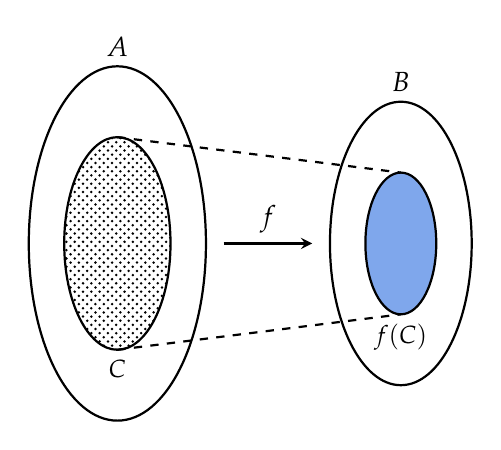
\begin{tikzpicture}[scale=0.9]
\draw[thick] (0,0) ellipse (1.25cm and 2.5cm);
\filldraw[pattern=crosshatch dots, thick] (0,0) ellipse (0.75cm and 1.5cm);

\draw[thick] (4,0) ellipse (1cm and 2cm);
\filldraw[fill=newblue, fill opacity=1/2, thick] (4,0) ellipse (0.5cm and 1cm);

\draw[thick,dashed] (0,1.5) -- (4,1);
\draw[thick,dashed] (0,-1.5) -- (4,-1);
\draw[->,thick] (1.5,0) -- (2.75,0) node[midway,above] {$f$};

\node[above] at (0,2.5) {$A$};
\node[above] at (4,2) {$B$};

\node[below] at (0,-1.5) {\small$C$};
\node[below] at (4,-1) {\small$f(C)$};
\end{tikzpicture}\]
\item[$\bullet$] The \cdef{preimage\ of} {\color{blue}$D$} \cdef{under} {\color{blue}$f$} is the set 
\[f^{-1}(D) \defeq \setp{y \in A}{f(y) \in D} \subseteq A\]
\[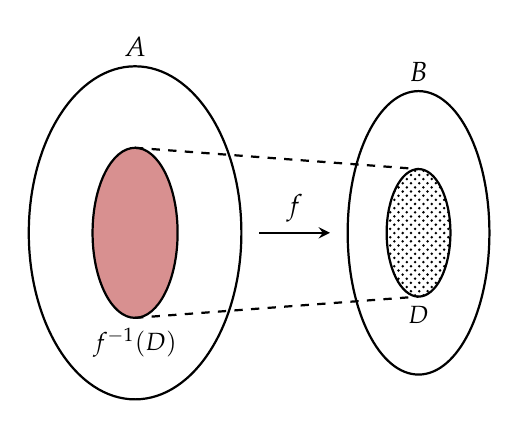
\begin{tikzpicture}[scale=0.9]
\draw[thick] (0,0) ellipse (1.5cm and 2.35cm);
\filldraw[fill=firebrick, fill opacity=1/2, thick] (0,0) ellipse (0.6cm and 1.2cm);

\draw[thick] (4,0) ellipse (1cm and 2cm);
\filldraw[pattern=crosshatch dots, thick] (4,0) ellipse (0.45cm and 0.9cm);

\draw[thick,dashed] (0,1.2) -- (4,0.9);
\draw[thick,dashed] (0,-1.2) -- (4,-0.9);
\draw[->,thick] (1.75,0) -- (2.75,0) node[midway,above] {$f$};

\node[above] at (0,2.35) {$A$};
\node[above] at (4,2) {$B$};

\node[below] at (0,-1.2) {\small$f^{-1}(D)$};
\node[below] at (4,-0.9) {\small$D$};
\end{tikzpicture}\]
\end{itemize}

\end{definition}

\vspace*{1em}

\begin{definition}
Let $A,B$ be non-empty sets. Define,
\[B^A = \setp{f:A \to B}{\text{$f$ is a function}}\]
\end{definition}

\vspace*{1em}

\begin{lemma}
For non-empty finite sets $A,B$, we have $|B^A| = \abs{B}^{\abs{A}}$.
\end{lemma}
\begin{proof}
Each element in $A$ has $\abs{B}$-many choices to be mapped to. Each such choice gives us a unique function. Since each element has $\abs{B}$-many choices, the total number of functions from $A$ to $B$ is
\[\underbrace{\abs{B} \cdot \abs{B} \cdots \abs{B}}_{\abs{A} \text{-times}} = \abs{B}^{\abs{A}}\]
This completes the proof. 
\end{proof}

\vspace*{1em}

\begin{definition}
Let $f:A \to B$  be a function.
\begin{itemize}
\item[$\bullet$] $f$ is said to be \cdef{injective} (or {\color{blue}\cdef{one}-\cdef{to}-\cdef{one}}) if ``$f$ maps distinct elements to distinct elements''; that is, if for every $x,y \in A,\ x \neq y$ implies $f(x) \neq f(y)$.
\[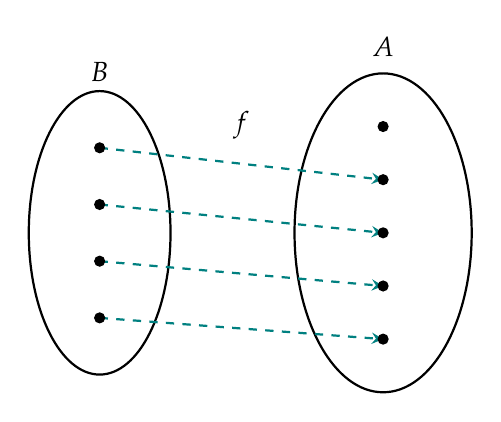
\begin{tikzpicture}[scale=0.9]
\draw[thick] (0,0) ellipse (1cm and 2cm);
\draw[thick] (4,0) ellipse (1.25cm and 2.25cm);

\draw[->,thick,dashed,teal] (0,1.2) -- (4,0.75) node[midway,above,yshift=5pt] {\color{black}$f$};
\draw[->,thick,dashed,teal] (0,0.4) -- (4,0);
\draw[->,thick,dashed,teal] (0,-0.4) -- (4,-0.75);
\draw[->,thick,dashed,teal] (0,-1.2) -- (4,-1.5);

\filldraw (0,1.2) circle (2pt);
\filldraw (0,0.4) circle (2pt);
\filldraw (0,-0.4) circle (2pt);
\filldraw (0,-1.2) circle (2pt);

\filldraw (4,1.5) circle (2pt);
\filldraw (4,0.75) circle (2pt);
\filldraw (4,0) circle (2pt);
\filldraw (4,-0.75) circle (2pt);
\filldraw (4,-1.5) circle (2pt);

\node[above] at (4,2.35) {$A$};
\node[above] at (0,2) {$B$};
\end{tikzpicture}\]
Equivalently, taking the contrapositive, $f$ is \cdef{injective} if for every $x,y \in A,\ f(x) = f(y)$ implies $x = y$. This definition is more convenient for proofs.\\
\\
$B$ has a ``copy of $A$ inside it''.

\item[$\bullet$] $f$ is said to be \cdef{surjective} (or \cdef{onto}) if $f(A) = B$.
\[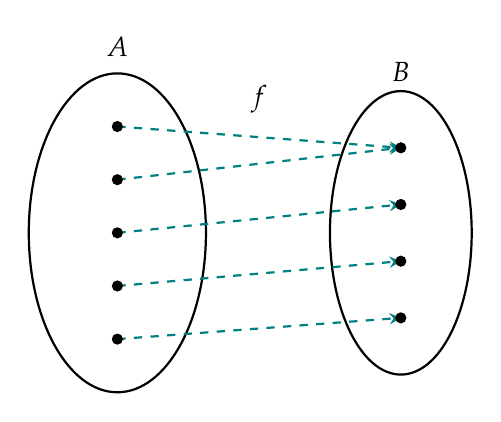
\begin{tikzpicture}[scale=0.9]
\draw[thick] (4,0) ellipse (1cm and 2cm);
\draw[thick] (0,0) ellipse (1.25cm and 2.25cm);

\draw[->,thick,dashed,teal] (0,1.5) -- (4,1.2) node[midway,above,yshift=5pt] {\color{black}$f$};
\draw[->,thick,dashed,teal] (0,0.75) -- (4,1.2);
\draw[->,thick,dashed,teal] (0,0) -- (4,0.4);
\draw[->,thick,dashed,teal] (0,-0.75) -- (4,-0.4);
\draw[->,thick,dashed,teal] (0,-1.5) -- (4,-1.2);

\filldraw (4,1.2) circle (2pt);
\filldraw (4,0.4) circle (2pt);
\filldraw (4,-0.4) circle (2pt);
\filldraw (4,-1.2) circle (2pt);

\filldraw (0,1.5) circle (2pt);
\filldraw (0,0.75) circle (2pt);
\filldraw (0,0) circle (2pt);
\filldraw (0,-0.75) circle (2pt);
\filldraw (0,-1.5) circle (2pt);

\node[above] at (0,2.35) {$A$};
\node[above] at (4,2) {$B$};
\end{tikzpicture}\]
Equivalently, ``if every element in $B$ is mapped to by $f$'', that is, for every $b \in B$, there exists an $a \in A$ such that $b = f(a)$ (this is just saying $B \subseteq f(A)$).%\\
%\\
%The set $A$ is ``partially collapsed'', in the sense that several elements of $A$ map to the same element of $B$, and all elements of $B$ are obtained in this way.

\item[$\bullet$] $f$ is \cdef{bijective} if it is both injective and surjective.
\[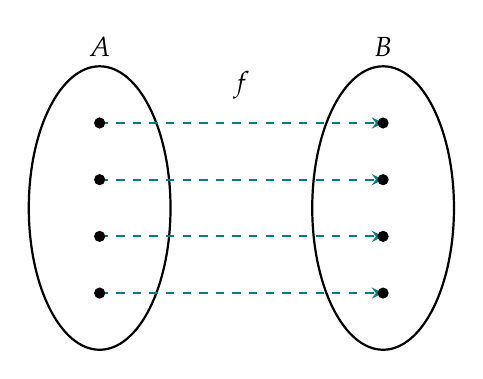
\begin{tikzpicture}[scale=0.9]
\draw[thick] (4,0) ellipse (1cm and 2cm);
\draw[thick] (0,0) ellipse (1cm and 2cm);

\draw[->,thick,dashed,teal] (0,1.2) -- (4,1.2) node[midway,above,yshift=5pt] {\color{black}$f$};
\draw[->,thick,dashed,teal] (0,0.4) -- (4,0.4);
\draw[->,thick,dashed,teal] (0,-0.4) -- (4,-0.4);
\draw[->,thick,dashed,teal] (0,-1.2) -- (4,-1.2);

\filldraw (4,1.2) circle (2pt);
\filldraw (4,0.4) circle (2pt);
\filldraw (4,-0.4) circle (2pt);
\filldraw (4,-1.2) circle (2pt);

\filldraw (0,1.2) circle (2pt);
\filldraw (0,0.4) circle (2pt);
\filldraw (0,-0.4) circle (2pt);
\filldraw (0,-1.2) circle (2pt);

\node[above] at (0,2) {$A$};
\node[above] at (4,2) {$B$};
\end{tikzpicture}\]
$f$ gives an exact correspondence of elements between $A$ and $B$. So sets $A$ and $B$ have the ``same size''. 
\end{itemize}
\end{definition}

\vspace*{1em}

\begin{example}
A function $f: \rr\setminus\set{2} \to \rr\setminus\set{3}$ is given by 
\[f(x) = 3 + \frac{6}{x - 2}\]
($f$ is not defined for $x = 2$ and its value can never be $3$).\\[0.5em]
Show that $f$ is a bijection.
\end{example}
\begin{proof}
We show $f$ is injective and bijective. To show $f$ is injective, suppose $x,y \neq 2$ are such that $f(x) = f(y)$, we want to show $x = y$. So, note
\begin{align*}
f(x) &= f(y)\\[0.5em]
3 + \frac{6}{x - 2} &= 3 + \frac{6}{y - 2}\\[0.5em]
\frac{6}{x - 2} &= \frac{6}{y - 2} &&& \text{subtracting $3$}\\[0.5em]
6(y - 2) &= 6(x - 2) &&& \text{cross-multiplying}\\[0.5em]
6y - 12 &= 6x - 12\\[0.5em]
\end{align*}
\begin{align*}
6y &= 6x &&& \text{adding $12$}\\[0.5em]
y &= x &&& \text{dividing by $6$}
\end{align*}
Thu, $f$ is injective.\\
\\
To show $f$ is surjective, let $b \in \rr\setminus\set{3}$. We show that there exists an element $a \in \rr\setminus\set{2}$ such that $f(a) = b$.\\

\begin{subproof}
\begin{proof}[Scratch work]\renewcommand{\qed}{}
We will work backwards to find such an $a$; suppose we did have $f(a) = b$, we solve for $a$.
\begin{align*}
3 + \frac{6}{a - 2} &= f(a) = b\\[0.5em]
\frac{6}{a - 2} &= b - 3 &&& \text{subtracting $3$}\\[0.5em]
\frac{a - 2}{6} &= \frac{1}{b - 3} &&& \text{taking reciprocal, we can since $b \neq 3$}\\[0.5em]
a - 2 &= \frac{6}{b - 3} &&& \text{multiplying by $6$}\\[0.5em]
a &= 2 + \frac{6}{b - 3} &&& \text{adding $2$}
\end{align*}
Note that this expression is $\neq 2$.
\end{proof}
\end{subproof}
\vspace*{0.5em}
For given $b$, consider
\[a = 2 + \frac{6}{b - 3} \in \rr\setminus\set{2}\]
This is such that 
\begin{align*}
f(a) &= 3 + \frac{6}{a - 2}\\[1em]
 &= 3 + \frac{6}{\left(2 + \frac{6}{b - 3}\right) - 2}\\[1em]
 &= 3 + \frac{6}{\frac{6}{b - 3}}\\[1em]
 &= 3 + \frac{6(b-3)}{6}\\[1em]
 &= 3 + (b-3)\\[0.5em]
 &= b
\end{align*}
Thus $f$ is surjective.\\
\\
This completes the proof. 
\end{proof}

\vspace*{1em}

\begin{discussion}
We can characterise injectivity and surjectivity in another way. Let $f:A \to B$ be a function. For any $b \in B$, we can consider its pre-image
\[f^{-1}(\set{b}) = \setp{a \in A}{f(a) = b}\]
$f$ is injective if and only if $|f^{-1}(\set{b})| \leq 1$ for every $b \in B$.\\[0.5em]
$f$ is surjective if and only if $|f^{-1}(\set{b})| \geq 1$ for every $b \in B$.\\[0.5em]
Therefore $f$ is bijective if and only if $|f^{-1}(\set{b})| = 1$.
\end{discussion}

\vspace*{1em}

\begin{definition}[Composition of Functions]
Let $f:A \to B$ and $g:B \to C$ be functions. Then their \cdef{composition} is the function
\[g\circ f: A \to C\]
defined as \[(g\circ f)(a) = g(f(a))\] for any $a \in A$.
\end{definition}

\vspace*{1em}

\begin{proposition}
Let $f:A \to B$ and $g:B \to C$ be functions.
\begin{itemize}
\item[(1)] If both $f$ and $g$ are injective, then their composition $g \circ f$ is also injective. 
\item[(2)] If both $f$ and $g$ are surjective, then their composition $g \circ f$ is also surjective. 
\end{itemize}
\end{proposition}
\[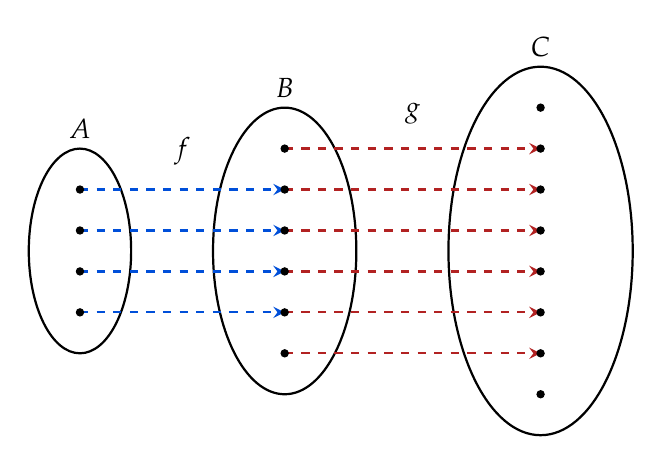
\begin{tikzpicture}[scale=0.65]
\draw[thick] (9,0) ellipse (1.8cm and 3.6cm);
\draw[thick] (4,0) ellipse (1.4cm and 2.8cm);
\draw[thick] (0,0) ellipse (1cm and 2cm);

\draw[->,thick,dashed,newblue] (0,1.2) -- (4,1.2) node[midway,above,yshift=5pt] {\color{black}$f$};
\draw[->,thick,dashed,newblue] (0,0.4) -- (4,0.4);
\draw[->,thick,dashed,newblue] (0,-0.4) -- (4,-0.4);
\draw[->,thick,dashed,newblue] (0,-1.2) -- (4,-1.2);

\draw[->,thick,dashed,firebrick] (4,2) -- (9,2) node[midway,above,yshift=5pt] {\color{black}$g$};
\draw[->,thick,dashed,firebrick] (4,1.2) -- (9,1.2);
\draw[->,thick,dashed,firebrick] (4,0.4) -- (9,0.4);
\draw[->,thick,dashed,firebrick] (4,-0.4) -- (9,-0.4);
\draw[->,thick,dashed,firebrick] (4,-1.2) -- (9,-1.2);
\draw[->,thick,dashed,firebrick] (4,-2) -- (9,-2);

\filldraw (9,2.8) circle (2pt);
\filldraw (9,2) circle (2pt);
\filldraw (9,1.2) circle (2pt);
\filldraw (9,0.4) circle (2pt);
\filldraw (9,-0.4) circle (2pt);
\filldraw (9,-1.2) circle (2pt);
\filldraw (9,-2) circle (2pt);
\filldraw (9,-2.8) circle (2pt);

\filldraw (4,2) circle (2pt);
\filldraw (4,1.2) circle (2pt);
\filldraw (4,0.4) circle (2pt);
\filldraw (4,-0.4) circle (2pt);
\filldraw (4,-1.2) circle (2pt);
\filldraw (4,-2) circle (2pt);

\filldraw (0,1.2) circle (2pt);
\filldraw (0,0.4) circle (2pt);
\filldraw (0,-0.4) circle (2pt);
\filldraw (0,-1.2) circle (2pt);

\node[above] at (0,2) {$A$};
\node[above] at (4,2.8) {$B$};
\node[above] at (9,3.6) {$C$};
\end{tikzpicture}\]
\begin{proof}[Proof of (1)]
Suppose $f$ and $g$ are injective, we need to show $g\circ f$ is injective. Consider any $x, y \in A$ such that $(g\circ f)(x) = (g\circ f)(y)$, we need to show $x = y$. We have,
\[g(f(x)) = g(f(y)),\]
since $g$ is injective, we have $f(x) = f(y)$. Now, since $f$ is injective, we obtain $x = y$.  Hence $g\circ f$ is injective.
\end{proof}
\[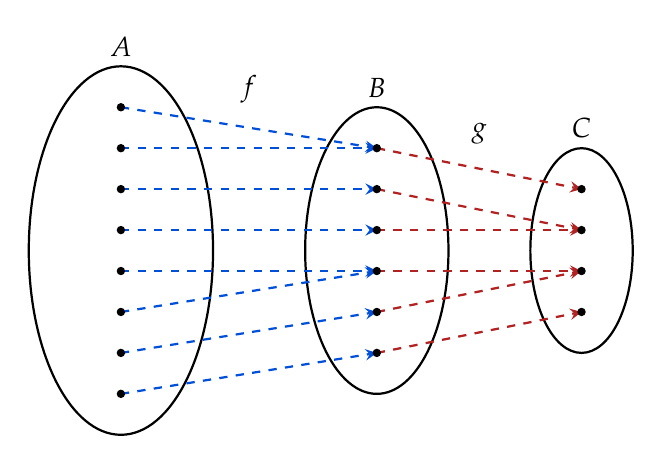
\begin{tikzpicture}[scale=0.65]
\draw[thick] (0,0) ellipse (1.8cm and 3.6cm);
\draw[thick] (5,0) ellipse (1.4cm and 2.8cm);
\draw[thick] (9,0) ellipse (1cm and 2cm);

\draw[->,thick,dashed,newblue] (0,2.8) -- (5,2) node[midway,above,yshift=5pt] {\color{black}$f$};
\draw[->,thick,dashed,newblue] (0,2) -- (5,2);
\draw[->,thick,dashed,newblue] (0,1.2) -- (5,1.2);
\draw[->,thick,dashed,newblue] (0,0.4) -- (5,0.4);
\draw[->,thick,dashed,newblue] (0,-0.4) -- (5,-0.4);
\draw[->,thick,dashed,newblue] (0,-1.2) -- (5,-0.4);
\draw[->,thick,dashed,newblue] (0,-2) -- (5,-1.2);
\draw[->,thick,dashed,newblue] (0,-2.8) -- (5,-2);

\draw[->,thick,dashed,firebrick] (5,2) -- (9,1.2) node[midway,above,yshift=5pt] {\color{black}$g$};
\draw[->,thick,dashed,firebrick] (5,1.2) -- (9,0.4);
\draw[->,thick,dashed,firebrick] (5,0.4) -- (9,0.4);
\draw[->,thick,dashed,firebrick] (5,-0.4) -- (9,-0.4);
\draw[->,thick,dashed,firebrick] (5,-1.2) -- (9,-0.4);
\draw[->,thick,dashed,firebrick] (5,-2) -- (9,-1.2);

\filldraw (0,2.8) circle (2pt);
\filldraw (0,2) circle (2pt);
\filldraw (0,1.2) circle (2pt);
\filldraw (0,0.4) circle (2pt);
\filldraw (0,-0.4) circle (2pt);
\filldraw (0,-1.2) circle (2pt);
\filldraw (0,-2) circle (2pt);
\filldraw (0,-2.8) circle (2pt);

\filldraw (5,2) circle (2pt);
\filldraw (5,1.2) circle (2pt);
\filldraw (5,0.4) circle (2pt);
\filldraw (5,-0.4) circle (2pt);
\filldraw (5,-1.2) circle (2pt);
\filldraw (5,-2) circle (2pt);

\filldraw (9,1.2) circle (2pt);
\filldraw (9,0.4) circle (2pt);
\filldraw (9,-0.4) circle (2pt);
\filldraw (9,-1.2) circle (2pt);

\node[above] at (9,2) {$C$};
\node[above] at (5,2.8) {$B$};
\node[above] at (0,3.6) {$A$};
\end{tikzpicture}\]
\begin{proof}[Proof of (2)]
Suppose $f$ and $g$ are surjective, we need to show $g\circ f$ is surjective. We aim to show that for every $c \in C$, we can find an $a \in A$ such that $(g\circ f)(a) = c$.\\[0.5em]
Consider any $c \in C$, since $g$ is surjective, there exists a $b \in B$ such that $g(b) = c$. Since $f$ is surjective, for this $b$, there exists an $a \in A$ such that $f(a) = b$. Hence, \[(g\circ f)(a) = g(f(a)) = g(b) = c.\] Thus $g\circ f$ is surjective. 
\end{proof}

\vspace*{1em}

What about the converse?
\begin{proposition}\label{thm:compinsur}
Let $f:A \to B$ and $g:B \to C$ be functions.
\begin{itemize}
\item[(1)] If $g \circ f$, then $f$ is injective. 
\[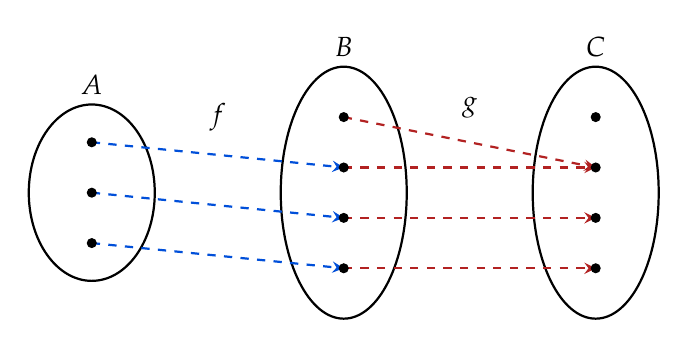
\begin{tikzpicture}[scale=0.8]
\draw[thick] (0,0) ellipse (1cm and 1.4cm);
\draw[thick] (4,0) ellipse (1cm and 2cm);
\draw[thick] (8,0) ellipse (1cm and 2cm);

\draw[->,thick,dashed,newblue] (0,0.8) -- (4,0.4) node[midway,above,yshift=5pt] {\color{black}$f$};
\draw[->,thick,dashed,newblue] (0,0) -- (4,-0.4);
\draw[->,thick,dashed,newblue] (0,-0.8) -- (4,-1.2);

\draw[->,thick,dashed,firebrick] (4,1.2) -- (8,0.4) node[midway,above,yshift=5pt] {\color{black}$g$};
\draw[->,thick,dashed,firebrick] (4,0.4) -- (8,0.4);
\draw[->,thick,dashed,firebrick] (4,-0.4) -- (8,-0.4);
\draw[->,thick,dashed,firebrick] (4,-1.2) -- (8,-1.2);

\filldraw (0,0.8) circle (2pt);
\filldraw (0,0) circle (2pt);
\filldraw (0,-0.8) circle (2pt);

\filldraw (4,1.2) circle (2pt);
\filldraw (4,0.4) circle (2pt);
\filldraw (4,-0.4) circle (2pt);
\filldraw (4,-1.2) circle (2pt);

\filldraw (8,1.2) circle (2pt);
\filldraw (8,0.4) circle (2pt);
\filldraw (8,-0.4) circle (2pt);
\filldraw (8,-1.2) circle (2pt);

\node[above] at (8,2) {$C$};
\node[above] at (4,2) {$B$};
\node[above] at (0,1.4) {$A$};
\end{tikzpicture}\]
\[\text{\emph{$g$ need not be injective in (1)}}\]
\item[(2)] If $g \circ f$ is surjective, then $g$ is surjective.
\[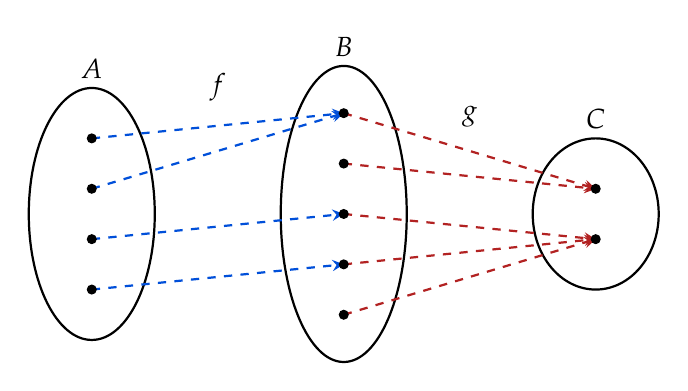
\begin{tikzpicture}[scale=0.8]
\draw[thick] (0,0) ellipse (1cm and 2cm);
\draw[thick] (4,0) ellipse (1cm and 2.35cm);
\draw[thick] (8,0) ellipse (1cm and 1.2cm);

\draw[->,thick,dashed,newblue] (0,1.2) -- (4,1.6) node[midway,above,yshift=5pt] {\color{black}$f$};
\draw[->,thick,dashed,newblue] (0,0.4) -- (4,1.6);
\draw[->,thick,dashed,newblue] (0,-0.4) -- (4,0);
\draw[->,thick,dashed,newblue] (0,-1.2) -- (4,-0.8);

\draw[->,thick,dashed,firebrick] (4,1.6) -- (8,0.4) node[midway,above,yshift=5pt] {\color{black}$g$};
\draw[->,thick,dashed,firebrick] (4,0.8) -- (8,0.4);
\draw[->,thick,dashed,firebrick] (4,0) -- (8,-0.4);
\draw[->,thick,dashed,firebrick] (4,-0.8) -- (8,-0.4);
\draw[->,thick,dashed,firebrick] (4,-1.6) -- (8,-0.4);

\filldraw (0,1.2) circle (2pt);
\filldraw (0,0.4) circle (2pt);
\filldraw (0,-0.4) circle (2pt);
\filldraw (0,-1.2) circle (2pt);

\filldraw (4,1.6) circle (2pt);
\filldraw (4,0.8) circle (2pt);
\filldraw (4,0) circle (2pt);
\filldraw (4,-0.8) circle (2pt);
\filldraw (4,-1.6) circle (2pt);

\filldraw (8,0.4) circle (2pt);
\filldraw (8,-0.4) circle (2pt);

\node[above] at (8,1.2) {$C$};
\node[above] at (4,2.35) {$B$};
\node[above] at (0,2) {$A$};
\end{tikzpicture}\]
\[\text{\emph{$f$ need not be surjective in (2)}}\]
\end{itemize}
\end{proposition}

\begin{proof}[Proof of (1)]
Suppose $g\circ f$ is injective, we need to show $f$ is injective. Consider any $x, y \in A$ such that $f(x) = f(y)$, we need to show $x = y$.\\[0.5em] 
Since $f(x) = f(y)$, therefore $g(f(x)) = g(f(y))$. That is,
\[g(f(x)) = g(f(y)).\]
Since $g\circ f$ is injective, we obtain $x = y$.  Hence $f$ is injective.
\end{proof}
\begin{proof}[Proof of (2)]
Suppose $g\circ f$ is surjective, we need to show $g$ is surjective. We aim to show that for every $c \in C$, we can find an $b \in B$ such that $g(b) = c$.\\[0.5em]
Consider any $c \in C$, since $g\circ f$ is surjective, there exists a $a \in A$ such that $(g\circ f)(a) = c$. Define $b = f(a)$, then $g(b) = g(f(a)) = (g\circ f)(a) = c$. Hence $g$ is surjective. 
\end{proof}

\vspace*{1em}

\begin{definition}
Two functions $f$ and $g$ are said to be equal, denoted $f = g$ if
\begin{itemize}
\item[(1)] $\dom f = \dom g$; and
\item[(2)] $f(x) = g(x)$ for every $x \in \dom f = \dom g$.
\end{itemize}
\end{definition}

\vspace*{1em}

\begin{theorem}
Let $f:A \to B$ and $g:B \to A$ be functions. Suppose,
\[g\circ f = \id_A \quad \text{and} \quad f\circ g = \id_B\]
Then $f$ and $g$ are bijective, and are inverses of each other as relations.\\[0.5em]
\emph{We call $g$ the \emph{inverse function} of $f$ (or vice versa)}.
\end{theorem}
\begin{remark}
Often the most convenient way to show a function $f:A \to B$ is bijective is to find a function $g:B \to A$ such that $f\circ g = \id_B$ and $g\circ f = \id_A$. If we can find such a function, we do not have give a separate argument on the injectivity and surjectivity of $f$. 
\end{remark}
\begin{proof}
Since the identity functions are bijective, we obtain that $g\circ f$ and $f\circ g$ are both bijective. In particular, $g\circ f$ and $f \circ g$ are injective, therefore by Theorem \ref{thm:compinsur} (1), we obtain $f$ and $g$ are injective respectively. We also have that $g\circ f$ and $f \circ g$ are surjective, therefore by Theorem \ref{thm:compinsur} (2), we obtain $f$ and $g$ are surjective. Hence, both $f$ and $g$ are injective and surjective, and thus bijective.\\
\\
Since $g\circ f = \id_A$, one can show by set inclusion arguments that as relations $g = f^{-1}$, where $f^{-1}$ is the inverse relation of $f$. That is, in this case the relation $f^{-1}$ is a function (in fact, $f^{-1}$ is a function if and only if $f$ is bijective).
\end{proof}

\vspace*{1em}

\begin{example}
A function $f: \rr\setminus\set{2} \to \rr\setminus\set{3}$ is given by 
\[f(x) = 3 + \frac{6}{x - 2}\]
Show that $f$ is a bijection.
\end{example}
\begin{proof}
We produce an inverse function to prove $f$ is bijective.\\
\begin{subproof}
\begin{proof}[Scratch work]\renewcommand{\qed}{}
We do some algebra to obtain the inverse function. 
\begin{itemize}[leftmargin=3.5em]
\item[Step 1.] First let $y = f(x)$, that is,
\[y = 3 + \frac{6}{x - 2}\]
\item[Step 2.] Replace $x$ by $y$ and vice versa. That is,
\[x = 3 + \frac{6}{y - 2}\]
\item[Step 3.] Solve for $y$.
\begin{align*}
3 + \frac{6}{y - 2} &= x\\[0.5em]
\frac{6}{y - 2} = x - 3 &&& \text{subtracting $3$}\\[0.5em]
\frac{y - 2}{6} = \frac{1}{x - 3} &&& \text{taking reciprocal, we can since $b \neq 3$}\\[0.5em]
y - 2 = \frac{6}{x - 3} &&& \text{multiplying by $6$}\\[0.5em]
y = 2 + \frac{6}{x - 3} &&& \text{adding $2$}
\end{align*}
Note that this expression is $\neq 2$.
\item[Step 4.] The resulting $y$ is your candidate for an inverse function.
\end{itemize}
\end{proof}
\end{subproof}
\vspace*{0.5em}
Define $g: \rr\setminus\set{3} \to \rr\setminus\set{2}$ as
\[g(x) = 2 + \frac{6}{x - 3}\]
Then,
\begin{align*}
(g\circ f)(x) = g(f(x)) &= 2 + \frac{6}{f(x) - 3} & (f\circ g)(x) = f(g(x)) &= 3 + \frac{6}{g(x) - 2}\\[1em]
 &= 2 + \frac{6}{\left(3 + \dfrac{6}{x - 2}\right) - 3} & &= 3 + \frac{6}{\left(2 + \dfrac{6}{x - 3}\right) - 2}\\[1em]
 &= 2 + \frac{6}{\left(\dfrac{6}{x - 2}\right)} & &= 3 + \frac{6}{\left(\dfrac{6}{x - 3}\right)}\\[1em]
 &= 2 + \frac{6(x-2)}{6} & &= 3 + \frac{6(x-3)}{6}\\[1em]
 &= 2 + (x - 2) = x & &= 3 + (x - 3)  = x
\end{align*}
Hence $f\circ g = \id$ and $g\circ f = \id$. Thus $f$ is bijective.
\end{proof}

\vspace*{1em}

\begin{remark}[Common Notations]
We commonly also use the word \emph{map} to mean a function, and if $b = f(a)$, we say \emph{$a$ maps to $b$ under $f$}, the symbolic notation for which is $a\mapsto b$, as we have seen.\\
\\
Given a function $f:A \to B$, if
\begin{itemize}
\item $f$ is injective, then one often writes this as $f:A \hookrightarrow B$.
\item $f$ is surjective, then one often writes this as $f:A\twoheadrightarrow B$.
\item $f$ is bijective, then one often writes this as $f: A \overset{\!\!\sim}{\to} B$.
\end{itemize}
\end{remark}
\newpage

\section{Cardinality of Sets}
\vspace*{1em}

\begin{discussion}
We want to ``count the number of elements in a set''. For finite sets, we simply do that, count the number of elements in the set. For infinite sets, how do we ``count''? There are many sets with infinitely many elements ; for example
\[\nn \subsetneq \zz \subsetneq \qq \subsetneq \rr \subsetneq \cc\]
are infinite sets. Here $\nn \defeq \zz_{>0} = \set{1,2,3,\ldots}$. How can we compare the number of elements in these sets? Since the above sets are related by proper inclusions, we may expect there are different levels of infinity.
\end{discussion}

\vspace*{1em}

\begin{lemma}
Let $A,B$ be finite sets, then $\abs{A} = \abs{B}$ if and only if there exists a bijection $f:A \to B$.
\end{lemma}
\begin{proof}\hfill
\begin{itemize}
\item[$(\Rightarrow)$] Suppose $\abs{A} = \abs{B} = n$; write $A = \set{a_1,\ldots,a_n}$ and $B = \set{b_1,\ldots,b_n}$. Define the function
\[f:A \to B,\ a_i \mapsto b_i,\]
this is evidently a bijection.

\item[$(\Leftarrow)$] Suppose there exists a bijection $f:A \to B$. Let $\abs{A} = n$; write $A = \set{a_1,\ldots,a_n}$. Since $f$ is a bijection, it is in particular an injection, therefore $f(A) = \set{f(a_1),\ldots,f(a_n)}$ is such that $|f(A)| = n$. Since $f$ is also surjective, $f(A) = B$, and hence $|B| = n$. \end{itemize}
%This completes the proof.
\vspace*{-\baselineskip}
\end{proof}

\vspace*{1em}

This motivates the following general definition.
\begin{definition}
Let $A,\,B$ be sets. $A$ and $B$ are said to be \cdef{numerically\ equivalent} (or {\color{blue}have the same \cdef{cardinality}}, or {\color{blue}have the same number of elements}), denoted $\abs{A} = \abs{B}$, if there exits a bijection
\[f:A \to B\]
If $A$ is finite with $n$-many elements, we write $|A| = n$.
\end{definition}

\vspace*{1em}

\begin{theorem}\label{thm:num-eq}
Numerical equivalence is a equivalence relation among sets. 
%The equivalence class of a set $A$ is denoted $\abs{A}$.
\end{theorem}

\vspace*{1em}

\begin{definition}
Let $A$ be a set.
\begin{itemize}
\item[$\bullet$] $A$ is said to be \cdef{denumerable} if $\abs{A} = \abs{\nn}$, that is, if there exists a bijection
\[f:\nn \to A\]
This means we can enumerate, label with positive integers, the elements of $A$. So, we can write $A = \set{a_1,a_2,\ldots}$.
\item[$\bullet$] $A$ is said to be \cdef{countable} if $\abs{A} < \infty$ or $\abs{A} = \abs{\nn}$, that is, if $A$ is finite or denumerable. 
\item[$\bullet$] $A$ is said to be \cdef{uncountable} if $A$ is not countable.
\end{itemize}
\end{definition}

\vspace*{1em}

\begin{discussion}
We will soon see that there are different levels of infinity, different infinite cardinalities. We will try and see that
\[\underbrace{\abs{\nn} = \abs{\zz} = \abs{\qq}}_{\text{denumerable}} < \abs{\rr} = \abs{\rr \times \rr} = \abs{\rr \times \rr \times \rr} \underbrace{< (?) < (??) < \cdots  < (?!?!?!) < \cdots}_{\text{these sets do exist}}\]
\begin{itemize}
\item $\abs{\nn} < \abs{\rr}$ was proved by Cantor using \emph{Cantor's diagonal argument}.
\item $\abs{\rr} = \abs{\rr^n}$, that is, there exists a bijection $f:\rr \to \rr^n$. It is enough to show $\abs{\rr} = \abs{\rr^2}$, that is, the real line and the plane have the same number of points, this is done by considering \emph{space-filling curves} (or \emph{Peano curves}).
\end{itemize}
\vspace*{0.5em}
{\bf Continuum Hypothesis.} Can there be an infinite set $A$ such that $\abs{\nn} < \abs{A} < \abs{\rr}$.
\end{discussion}

\vspace*{1em}

\begin{theorem}\label{thm:sub-count}\hfill
\begin{itemize}
\item[(1)] An infinite subset of a denumerable set is denumerable.
\item[(2)] A cartesian product of denumerable sets is denumerable.
\end{itemize}
\end{theorem}
\begin{proof}[Proof of Theorem \ref{thm:sub-count}(1)]
Let $A$ be a denumerable set and let $S \subseteq A$ be infinite. Then, by definition, there exists a bijection
\[f:\nn \to A\]
Consider $f^{-1}(S) \subseteq \nn$, necessarily infinite, we order the elements in this set as 
\[k_1 < k_2 < \cdots < k_n < \cdots\]
Then, we can define a bijection
\[g:\nn \to f^{-1}(S),\ i \mapsto k_i\]
Thus, $\abs{\nn} = |f^{-1}(S)|$.\\
\\
Now, note that the function
\[f^{-1}(S) = \setp{k \in \nn}{f(k) \in S} \to S: k \mapsto f(k)\]
is a bijection; and hence $|f^{-1}(S)| = |S|$.\\
\\
Thus, $\abs{S} = \abs{\nn}$ (as numerical equivalence is, in particular, transitive, by Theorem \ref{thm:num-eq}) and therefore $S$ is denumerable.
\end{proof}

\vspace*{1em}

\begin{example}
$2\nn$, the set of even numbers, is denumerable. One can explicitly also give a bijection
\[2\nn \to \nn:n \mapsto n/2\]
\end{example}

%\vspace*{1em}

\begin{remark}\label{rmk:inj-count}
Theorem \ref{thm:sub-count} (1) tells us that, for an infinite set $A$, it is enough to exhibit an \emph{injective function} $f:A \to X$, where $X$ is denumerable, to conclude $A$ is denumerable.\\
\\
Since if $f$ is injective, then $f:A \to f(A)$ is a bijection, so $\abs{A} = \abs{f(A)}$. Since $A$ is infinite, so is $f(A)$. Now, $f(A)$ is an infinite subset of $X$, a denumerable set, and is therefore denumerable.
\end{remark}

\vspace*{1em}

\begin{proposition}
$\abs{\zz} = \abs{\nn}$
\end{proposition}
\begin{proof}[Strategy]\renewcommand{\qed}{}
Our strategy is the following: we will send even numbers to positive integers, and odd numbers to non-positive integers.
\[\begin{tikzcd}[scale=0.75]
{\color{firebrick}1} \arrow[dd, maps to] & {\color{newblue}2} \arrow[d, maps to] & {\color{firebrick}3} \arrow[dd, maps to] & {\color{newblue}4} \arrow[d, maps to] & {\color{firebrick}5} \arrow[dd, maps to] & {\color{newblue}6} \arrow[d, maps to] & {\color{firebrick}7} \arrow[dd, maps to] & {\color{newblue}8} \arrow[d, maps to] & {\color{firebrick}9} \arrow[dd, maps to] & \cdots \\[-0.5em]
                                         & {\color{newblue}1}                    &                                          & {\color{newblue}2}                    &                                          & {\color{newblue}3}                    &                                          & {\color{newblue}4}                    &                                          & \cdots \\[-1em]
{\color{firebrick}0}                     &                                       & {\color{firebrick}-1}                    &                                       & {\color{firebrick}-2}                    &                                       & {\color{firebrick}-3}                    &                                       & {\color{firebrick}-4}                    & \cdots
\end{tikzcd}\]
\end{proof}
\begin{proof}
We explicitly construct a bijection $\nn \to \zz$. Consider the function
\[f:\nn \to \zz,\ n \mapsto \begin{cases}
\dfrac{n}{2} & \text{if $n$ is even}\\[1.5em]
\dfrac{1 - n}{2} & \text{if $n$ is odd}
\end{cases}\]
One directly verifies that this is a bijection.
\end{proof}

\vspace*{1em}

\begin{proof}[Proof of Theorem \ref{thm:sub-count}(2)]\renewcommand{\qed}{}
Let $A$ and $B$ be two denumerable sets. Then we can order elements of $A$ and $B$ as
\begin{align*}
A &= \set{a_1,a_2,a_3,\ldots,a_n,\ldots}\\[0.5em]
B &= \set{b_1,b_2,b_3,\ldots,b_n,\ldots}
\end{align*}
Then we can order $A \times B$ as follows\\

\begin{minipage}{0.7\textwidth}
\[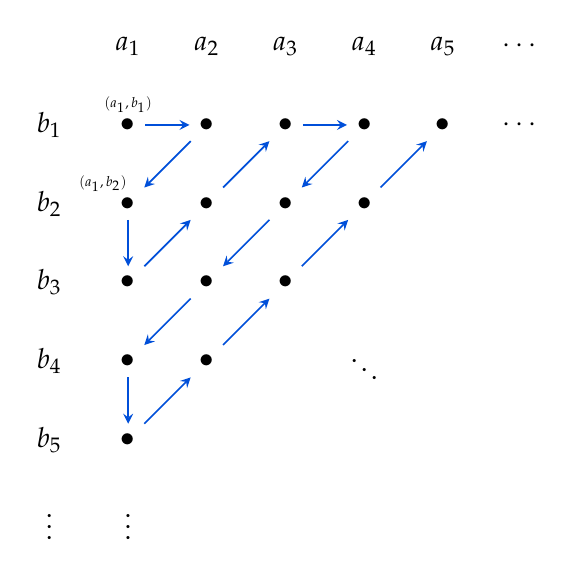
\begin{tikzpicture}
	\node at (0,6) {$a_1$};
	\node at (1,6) {$a_2$};
	\node at (2,6) {$a_3$};
	\node at (3,6) {$a_4$};
	\node at (4,6) {$a_5$};
	\node at (5,6) {$\cdots$};

	\node at (-1,5) {$b_1$};
	\node at (-1,4) {$b_2$};
	\node at (-1,3) {$b_3$};
	\node at (-1,2) {$b_4$};
	\node at (-1,1) {$b_5$};
	\node at (-1,0) {$\vdots$};

	\node (A) at (0,5) {$\bullet$};
	\node[above,yshift=1pt] at (0,5) {\tiny$(a_1,b_1)$};
	\node (B) at (1,5) {$\bullet$};
	\node (C) at (2,5) {$\bullet$};
	\node (D) at (3,5) {$\bullet$};
	\node (E) at (4,5) {$\bullet$};

	\node (F) at (0,4) {$\bullet$};
	\node[above left,xshift=3pt,yshift=1pt] at (0,4) {\tiny$(a_1,b_2)$};
	\node (G) at (1,4) {$\bullet$};
	\node (H) at (2,4) {$\bullet$};
	\node (I) at (3,4) {$\bullet$};
	
	\node (J) at (0,3) {$\bullet$};
	\node (K) at (1,3) {$\bullet$};
	\node (L) at (2,3) {$\bullet$};

	\node (M) at (0,2) {$\bullet$};
	\node (N) at (1,2) {$\bullet$};

	\node (O) at (0,1) {$\bullet$};

	\draw[->,semithick,newblue] (A)--(B);
	\draw[->,semithick,newblue] (B)--(F);
	\draw[->,semithick,newblue] (F)--(J);
	\draw[->,semithick,newblue] (J)--(G);
	\draw[->,semithick,newblue] (G)--(C);
	\draw[->,semithick,newblue] (C)--(D);
	\draw[->,semithick,newblue] (D)--(H);
	\draw[->,semithick,newblue] (H)--(K);
	\draw[->,semithick,newblue] (K)--(M);
	\draw[->,semithick,newblue] (M)--(O);
	\draw[->,semithick,newblue] (O)--(N);
	\draw[->,semithick,newblue] (N)--(L);
	\draw[->,semithick,newblue] (L)--(I);
	\draw[->,semithick,newblue] (I)--(E);
	
	\node at (0,0) {$\vdots$};
	\node at (5,5) {$\cdots$};
	\node at (3,2) {$\ddots$};
\end{tikzpicture}\]
\end{minipage}\hspace*{-3em}
\begin{minipage}{0.3\textwidth}
\raisebox{0.15em}{$\begin{tikzpicture} \draw[->,semithick,newblue] (0.5,0)--(1,0); \end{tikzpicture}$} gives us one way to order all elements in $A \times B$, hence $\abs{\nn} = \abs{A \times B}$.\hfill$\square$
\end{minipage}
\end{proof}

%\vspace*{1em}

\begin{discussion}
We saw that $\abs{\zz} = \abs{\nn}$. This is a common phenomenon with infinite sets, and a property not shared with finite sets: infinite sets may have the same cardinality as a proper subsets.\\
\\
Our goal now is to prove $\abs{\qq} = \abs{\nn}$ and $\abs{\nn} < \abs{\rr}$. That is, that $\qq$ is denumerable and $\rr$ is uncountable.
\end{discussion}

\vspace*{1em}

\begin{theorem}
The set $\qq$ is countable. 
\end{theorem}
\begin{proof}
We will show that there is a injective map from $\qq$ to a denumerable set, and we will have proven that $\qq$ is denumerable as per Remark \ref{rmk:inj-count}.\\
\\
Note that any rational number $r \in \qq$ can be written in its reduced form, that is, as
\[r = \frac{a}{b},\quad \text{$a \in \zz$, $b \in \nn$, and $a$ and $b$ have no common factors}\]
Then we have the following injective function
\[f:\qq = \left\{\frac{a}{b}\ \big\vert\; \frac{a}{b}\text{ is in reduced form}\right\} \to \zz \times \nn,\ \frac{a}{b} \mapsto (a,b)\]
Note that this map is not surjective, since, for example, $(4,6) \in \zz \times \nn$ is not in the range of $f$ because
\[\frac{4}{6} = \frac{2}{3},\;\text{ and }\; f\left(\frac{2}{3}\right) = (2,3)\]
In any case, this completes the proof.
\end{proof}

\vspace*{2em}

\begin{mdframed}
\begin{center}
{\Large Uncountable Sets}
\end{center}
\end{mdframed}

\begin{theorem}
The open interval $(0,1)$ has the same cardinality as $\rr$.
\end{theorem}
\begin{proof}
The main idea is to find a function that 	``stretches $(0,1)$'' to $\rr$. Consider the function
\[f:(0,1) \to \rr,\; x \mapsto -\frac{1}{x} + \frac{1}{1 - x}\]
It's straightforward to show it is injective but for surjectivity we are forced to revert to some limit arguments that are beyond the scope of this course. To convince yourself, you can graph the function and see that the range is indeed all of $\rr$.\\
\\
Thus, $\abs{(0,1)} = \abs{\rr}$.
\end{proof}

\vspace*{1em}

\begin{theorem}
$\abs{\nn} < \abs{\rr}$
\end{theorem}
\begin{proof}
In view of the previous theorem, it suffices to show that $\abs{\nn} < \abs{(0,1)}$. For the sake of contradiction, assume $\abs{(0,1)} = \abs{\nn}$. That is, there exists a bijection
\[f:\nn \to (0,1)\]\newpage
We examine the range of $f$. Any real number $0 < r < 1$ has a decimal expansion. If $r$ is irrational, then it has a unique decimal expansion. On the other hand, if $r$ is rational, then it can have two possible decimal expansions; for example,
\[0.4000000\ldots = 0.399999\ldots\]
In this case, we choose the expansion with a string of $0$'s from some point on. Thus, for every element in the range of $f$ (which is all of $(0,1)$ as $f$ is surjective), we can choose a distinct decimal expansion
\begin{align*}
f(1) &= a_1 = 0.{\color{firebrick}a_{11}}a_{12}a_{13}a_{14}\ldots\\[0.5em]
f(2) &= a_2 = 0.a_{21}{\color{firebrick}a_{22}}a_{13}a_{14}\ldots\\[0.5em]
f(3) &= a_3 = 0.a_{31}a_{32}{\color{firebrick}a_{33}}a_{34}\ldots\\[0.5em]
f(4) &= a_4 = 0.a_{41}a_{42}a_{43}{\color{firebrick}a_{44}}\ldots\\
	 & \qquad\qquad\vdots
\end{align*}
Cantor chose to examine the diagonal entries to produce an element in $(0,1)$ that is part of this list, that is, not contained in the range of $f$, thereby contradicting its surjectivity.\\
\\
Consider a sequence $\set{b_n}_{n \geq 1}$, where for each $n$, we have $0 \leq b_n \leq 9$, given by 
\[b_k = \begin{cases}
a_{kk} + 1 & \text{if $0 \leq a_{kk} < 9$}\\[0.5em]
0 & \text{if $a_{kk} = 9$}
\end{cases}\]
Consider the real number
\[b = 0.b_1b_2b_3b_4\ldots\]
Note that for each $n$, $b \neq f(n) = a_n$, since they have different $n^{\text{th}}$ digits in their decimal expansion. We have produced an $b \in (0,1)$ but $b \notin f(\nn)$ and hence $f(\nn) \neq \rr$, contradicting the surjectivity of $f$. Thus, $\abs{\nn} < \abs{(0,1)} = \abs{\rr}$.
\end{proof}
\newpage



%\appendix
%\section{Index}
%\begin{minipage}{0.5\textwidth}
%{\bf Lecture 1.}
%\begin{itemize}
%\item Sets and their Notations (Page \pageref{set-notation})
%\item Empty Set (Page \pageref{empty-set})
%\item Cardinality (Page \pageref{cardinality})
%\item Subsets (Page \pageref{subsets})
%\item Equality of Sets (Page \pageref{equality-sets})
%\item Power Set (Page \pageref{power-set})
%\item Set Operations (Page \pageref{set-operations})
%\item Indexed Collection of Sets (Page \pageref{indexed-collection})
%\item Partition of Sets (Page \pageref{partition})
%\end{itemize}
%%\vspace*{1em}
%%{\bf Lecture 2.}
%%\begin{itemize}
%%\item Sets and their Notations
%%\item Empty Set 
%%\item Subsets
%%\item Power Set
%%\item Set Operations
%%\item Indexed Collection of Sets
%%\item Partition of Sets
%%\end{itemize}
%\end{minipage}
%\newpage

\thispagestyle{empty}
\nocite{chartrand2018mathematical}

\bibliographystyle{amsalpha}
\bibliography{citations.bib}
%
\vspace*{5em}
%
%\thispagestyle{empty}
\centering
\hrule
\vspace*{5em}
\begin{center}
\emph{Solving a problem for which you know there's an answer is like climbing a mountain with a guide, along a trail someone else has laid. In mathematics, the truth is somewhere out there in a place no one knows, beyond all the beaten paths. And it's not always at the top of the mountain. It might be in a crack on the smoothest cliff or somewhere deep in the valley.}
\end{center}
\vspace*{-1em}
\hfill {\small -- Yoko Ogawa, \textsl{The Housekeeper and the Professor}}
\vfill
\begin{center}
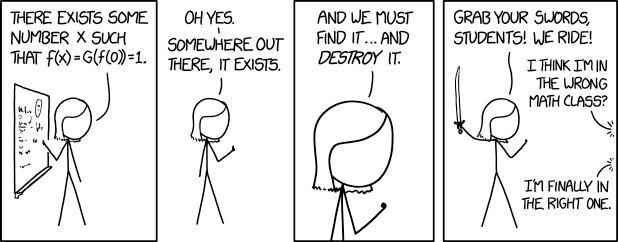
\includegraphics[scale=0.6]{existence_proof.png}\\[0.5em]
\href{https://xkcd.com/1856/}{\emph{Existence Proof} by xkcd}
\end{center}
\vfill
\vfill
\end{document}